\documentclass[12pt,a4paper,twocolumn]{article}
%\usepackage{psfrag}
\usepackage{tikz} % gestion de dessin directe
\usepackage{pgfplotstable, environ,subcaption,caption,framed,xspace,enumitem}
\usepackage{hyperref}
\usetikzlibrary{arrows,positioning}
\usetikzlibrary{plotmarks,matrix}
\usepackage{pgfplots,siunitx,multicol}
\pgfplotsset{compat=newest}
\usepackage[utf8]{inputenc}
\usepackage[T1]{fontenc}
\usepackage{amsmath,amssymb,mathrsfs,bm,cancel,geometry}
\usepackage{MnSymbol}
\usepackage{pgfplots}
\pgfplotsset{compat=1.11}
%\usepackage[spanish]{babel}
\usetikzlibrary{backgrounds,arrows.meta,external,babel,math,patterns,patterns.meta,calc,decorations.pathmorphing,decorations.markings, decorations.pathreplacing,shapes,fillbetween}

\begin{document}
Force signals can be acquired from the sensor integrated into the Arduino  system with a sampling frequency of \SI{80}{\hertz}. An example of such a signal is shown on Figure \ref{fig:FD_typical}. A dominant frequency and a mean value can be determined in order to characterize the dynamics of the Dshape body. For a set of velocities in the wind tunnel and a value of thickness (rigidity) and length $L = 1.50 D$ of the flexible plates, we   display the behavior of the signals which are proportional to the drag force in Figure \ref{fig:FD_series_crude}. Values must be corrected by subtracting those corresponding to the mounting structure. Nevertheless, by scaling the former with $u_\infty^2$, we can obtain magnitudes proportional to the drag coefficient $C_D$ as presented in Figure \ref{fig:CD}.

The determination fo the main frequencies in the force signals is obtained through Fourier analysis. Figure \ref{fig:FD_fourier}. shows the power spectral density of the signal as a function of the frequencies of the reference case, where there is no flexible flaps mounted on the body. Taking an order value of $St=0.2=f_{vs}D/u_\infty$, for $D=\SI{50}{\milli\meter}$ and $u_\infty=\SI{3.5}{\meter/\second}$, the vortex shedding frequency results $f_{vs}=\SI{14}{\hertz}$. Inspecting Figure \ref{fig:FD_fourier}, we can compare with the maximum peak found at $f_{\max}=\SI{12.67}{\hertz}$.

Fast camera images were recorded at a sampling frequency of $ \SI{250}{\micro\second}$. A particular snapshot is shown on Figure \ref{fig:snapshot} where we can determine the elastic deformation. produced by the flow. We are particularly interested in following the trailing edges displacement, so we can produce a stack of images for each time of acquisition at the regions of interest. The result is displayed on Figure \ref{fig:stack} where we can study the fluctuations, their frequency and compare with those produce by the forces on the body.

	\begin{figure}
	\centering\resizebox{.495\textwidth}{!}{%
		% This file was created with tikzplotlib v0.10.1.
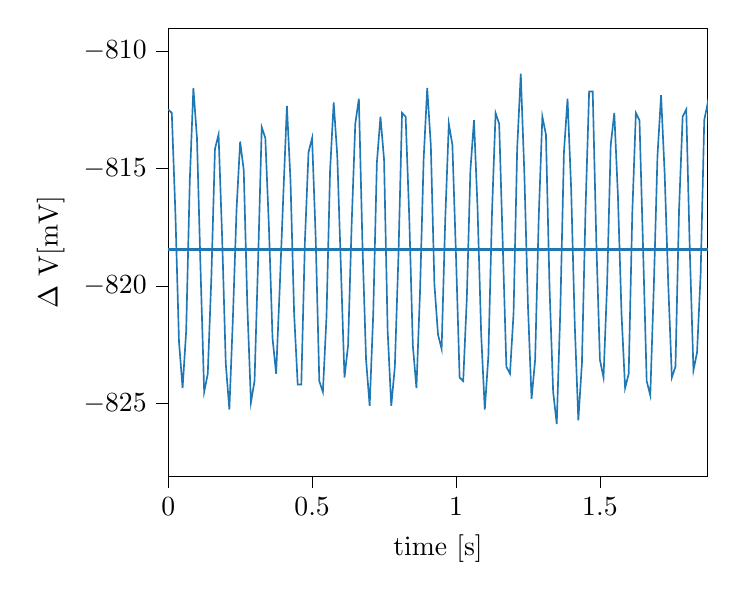
\begin{tikzpicture}

\definecolor{darkgray176}{RGB}{176,176,176}
\definecolor{steelblue31119180}{RGB}{31,119,180}

\begin{axis}[
tick align=outside,
tick pos=left,
x grid style={darkgray176},
xlabel={time [s]},
xmin=0, xmax=1.875,
xtick style={color=black},
y grid style={darkgray176},
ylabel={\(\displaystyle \Delta\) V[mV]},
ymin=-828.118, ymax=-809.022,
ytick style={color=black}
]
\addplot [semithick, steelblue31119180]
table {%
0 -812.48
0.0125 -812.63
0.025 -816.89
0.0375 -822.37
0.05 -824.35
0.0625 -821.92
0.075 -815.53
0.0875 -811.57
0.1 -813.7
0.1125 -819.33
0.125 -824.51
0.1375 -823.74
0.15 -819.63
0.1625 -814.16
0.175 -813.55
0.1875 -817.96
0.2 -823.29
0.2125 -825.27
0.225 -821.31
0.2375 -816.74
0.25 -813.85
0.2625 -815.07
0.275 -820.85
0.2875 -824.96
0.3 -824.05
0.3125 -818.87
0.325 -813.24
0.3375 -813.7
0.35 -817.5
0.3625 -822.22
0.375 -823.74
0.3875 -820.09
0.4 -816.13
0.4125 -812.33
0.425 -815.53
0.4375 -821.16
0.45 -824.2
0.4625 -824.2
0.475 -818.11
0.4875 -814.31
0.5 -813.7
0.5125 -817.96
0.525 -824.05
0.5375 -824.51
0.55 -821.31
0.5625 -815.07
0.575 -812.18
0.5875 -814.46
0.6 -819.18
0.6125 -823.9
0.625 -822.53
0.6375 -817.35
0.65 -813.09
0.6625 -812.02
0.675 -818.26
0.6875 -823.14
0.7 -825.11
0.7125 -821.16
0.725 -814.76
0.7375 -812.79
0.75 -814.61
0.7625 -821.92
0.775 -825.11
0.7875 -823.44
0.8 -818.72
0.8125 -812.63
0.825 -812.79
0.8375 -817.05
0.85 -822.53
0.8625 -824.35
0.875 -820.24
0.8875 -814.61
0.9 -811.57
0.9125 -814
0.925 -819.94
0.9375 -822.07
0.95 -822.68
0.9625 -817.2
0.975 -813.09
0.9875 -814
1 -818.72
1.0125 -823.9
1.025 -824.05
1.0375 -820.55
1.05 -815.07
1.0625 -812.94
1.075 -816.74
1.0875 -822.07
1.1 -825.27
1.1125 -822.98
1.125 -816.89
1.1375 -812.63
1.15 -813.09
1.1625 -818.26
1.175 -823.44
1.1875 -823.74
1.2 -821.16
1.2125 -814.16
1.225 -810.96
1.2375 -815.22
1.25 -820.85
1.2625 -824.81
1.275 -823.14
1.2875 -817.05
1.3 -812.79
1.3125 -813.55
1.325 -820.09
1.3375 -824.51
1.35 -825.88
1.3625 -821
1.375 -814.31
1.3875 -812.02
1.4 -815.83
1.4125 -821.61
1.425 -825.72
1.4375 -823.29
1.45 -816.74
1.4625 -811.72
1.475 -811.72
1.4875 -818.11
1.5 -823.14
1.5125 -823.9
1.525 -819.94
1.5375 -814
1.55 -812.63
1.5625 -816.13
1.575 -821.16
1.5875 -824.35
1.6 -823.74
1.6125 -816.89
1.625 -812.63
1.6375 -812.94
1.65 -818.42
1.6625 -824.05
1.675 -824.66
1.6875 -819.94
1.7 -814.46
1.7125 -811.87
1.725 -815.22
1.7375 -819.94
1.75 -823.9
1.7625 -823.44
1.775 -816.74
1.7875 -812.79
1.8 -812.48
1.8125 -818.57
1.825 -823.59
1.8375 -822.83
1.85 -819.48
1.8625 -812.94
1.875 -812.18
1.8875 -816.74
1.9 -821.92
1.9125 -825.88
1.925 -822.37
1.9375 -817.96
1.95 -812.63
1.9625 -814
1.975 -819.79
1.9875 -823.59
2 -824.35
2.0125 -819.94
2.025 -814.61
2.0375 -813.24
2.05 -816.44
2.0625 -822.53
2.075 -824.66
2.0875 -822.68
2.1 -816.13
2.1125 -811.11
2.125 -813.55
2.1375 -819.03
2.15 -823.9
2.1625 -823.9
2.175 -819.03
2.1875 -814.46
2.2 -812.18
2.2125 -816.29
2.225 -822.37
2.2375 -824.81
2.25 -821.77
2.2625 -815.68
2.275 -812.63
2.2875 -814.16
2.3 -820.4
2.3125 -824.2
2.325 -823.59
2.3375 -819.63
2.35 -813.24
2.3625 -812.18
2.375 -815.53
2.3875 -821.46
2.4 -824.96
2.4125 -821.77
2.425 -816.44
2.4375 -812.33
2.45 -813.55
2.4625 -820.09
2.475 -823.14
2.4875 -824.66
2.5 -819.63
2.5125 -814.16
2.525 -812.94
2.5375 -815.68
2.55 -821.61
2.5625 -824.35
2.575 -822.83
2.5875 -816.89
2.6 -812.18
2.6125 -814.92
2.625 -819.48
2.6375 -824.2
2.65 -823.9
2.6625 -818.87
2.675 -814.16
2.6875 -812.02
2.7 -816.74
2.7125 -821.61
2.725 -823.59
2.7375 -821.61
2.75 -815.53
2.7625 -813.55
2.775 -813.7
2.7875 -819.94
2.8 -824.96
2.8125 -824.2
2.825 -820.4
2.8375 -814.61
2.85 -813.24
2.8625 -817.66
2.875 -822.07
2.8875 -824.35
2.9 -821.61
2.9125 -816.44
2.925 -813.24
2.9375 -814.16
2.95 -819.03
2.9625 -822.98
2.975 -823.44
2.9875 -818.87
3 -812.94
3.0125 -813.09
3.025 -817.2
3.0375 -821.92
3.05 -824.05
3.0625 -820.4
3.075 -815.68
3.0875 -811.72
3.1 -814.16
3.1125 -821.16
3.125 -825.11
3.1375 -826.33
3.15 -820.24
3.1625 -814.16
3.175 -813.24
3.1875 -816.89
3.2 -823.44
3.2125 -824.66
3.225 -821.61
3.2375 -815.68
3.25 -811.42
3.2625 -815.07
3.275 -819.18
3.2875 -824.05
3.3 -822.68
3.3125 -817.96
3.325 -813.85
3.3375 -810.96
3.35 -817.2
3.3625 -822.22
3.375 -825.11
3.3875 -821.92
3.4 -814.31
3.4125 -812.33
3.425 -814.16
3.4375 -821
3.45 -824.35
3.4625 -823.29
3.475 -818.87
3.4875 -812.79
3.5 -811.87
3.5125 -816.74
3.525 -822.98
3.5375 -825.42
3.55 -820.4
3.5625 -814.92
3.575 -813.09
3.5875 -814.46
3.6 -819.79
3.6125 -823.9
3.625 -823.74
3.6375 -817.81
3.65 -813.24
3.6625 -814.61
3.675 -818.42
3.6875 -822.53
3.7 -824.05
3.7125 -820.85
3.725 -815.53
3.7375 -811.72
3.75 -814.76
3.7625 -820.24
3.775 -824.66
3.7875 -822.53
3.8 -816.89
3.8125 -813.09
3.825 -813.09
3.8375 -817.81
3.85 -822.07
3.8625 -823.74
3.875 -820.09
3.8875 -814.61
3.9 -812.18
3.9125 -815.37
3.925 -821.92
3.9375 -824.81
3.95 -823.59
3.9625 -817.5
3.975 -813.09
3.9875 -813.55
4 -818.87
4.0125 -823.9
4.025 -825.11
4.0375 -820.7
4.05 -814.46
4.0625 -811.72
4.075 -814.76
4.0875 -820.4
4.1 -823.9
4.1125 -822.22
4.125 -816.44
4.1375 -812.33
4.15 -812.48
4.1625 -818.42
4.175 -823.44
4.1875 -823.9
4.2 -820.55
4.2125 -813.39
4.225 -811.72
4.2375 -814.61
4.25 -821.31
4.2625 -825.11
4.275 -823.44
4.2875 -818.87
4.3 -813.39
4.3125 -813.24
4.325 -817.66
4.3375 -822.53
4.35 -824.05
4.3625 -819.79
4.375 -814.31
4.3875 -812.48
4.4 -816.44
4.4125 -821
4.425 -823.74
4.4375 -821.16
4.45 -815.68
4.4625 -811.87
4.475 -812.94
4.4875 -819.94
4.5 -824.35
4.5125 -825.57
4.525 -821.31
4.5375 -815.22
4.55 -813.39
4.5625 -816.29
4.575 -822.37
4.5875 -824.05
4.6 -822.37
4.6125 -817.2
4.625 -813.24
4.6375 -814.76
4.65 -819.33
4.6625 -823.74
4.675 -822.98
4.6875 -818.26
4.7 -812.63
4.7125 -810.96
4.725 -815.83
4.7375 -821
4.75 -824.66
4.7625 -822.68
4.775 -816.29
4.7875 -813.09
4.8 -813.7
4.8125 -819.18
4.825 -825.27
4.8375 -825.42
4.85 -820.7
4.8625 -815.37
4.875 -814.31
4.8875 -818.87
4.9 -822.22
4.9125 -825.11
4.925 -822.22
4.9375 -815.98
4.95 -810.65
4.9625 -811.72
4.975 -819.18
4.9875 -822.37
5 -823.14
5.0125 -818.42
5.025 -812.94
5.0375 -811.11
5.05 -814.31
5.0625 -821.46
5.075 -824.2
5.0875 -822.07
5.1 -817.2
5.1125 -812.79
5.125 -814.92
5.1375 -820.24
5.15 -824.51
5.1625 -825.72
5.175 -820.24
5.1875 -815.37
5.2 -812.79
5.2125 -816.59
5.225 -822.83
5.2375 -823.59
5.25 -823.29
5.2625 -814.76
5.275 -811.87
5.2875 -812.79
5.3 -816.44
5.3125 -822.68
5.325 -820.55
5.3375 -819.18
5.35 -813.24
5.3625 -812.33
5.375 -818.42
5.3875 -822.37
5.4 -826.18
5.4125 -822.53
5.425 -816.89
5.4375 -813.09
5.45 -814.92
5.4625 -821.77
5.475 -825.11
5.4875 -823.74
5.5 -819.79
5.5125 -814.16
5.525 -813.09
5.5375 -815.98
5.55 -821.16
5.5625 -823.59
5.575 -819.63
5.5875 -815.07
5.6 -811.57
5.6125 -815.07
5.625 -820.55
5.6375 -823.14
5.65 -823.9
5.6625 -817.96
5.675 -814
5.6875 -812.79
5.7 -818.26
5.7125 -825.57
5.725 -825.57
5.7375 -823.29
5.75 -816.89
5.7625 -814.31
5.775 -816.59
5.7875 -819.03
5.8 -824.51
5.8125 -823.44
5.825 -817.81
5.8375 -812.33
5.85 -810.65
5.8625 -817.2
5.875 -820.85
5.8875 -822.22
5.9 -819.94
5.9125 -813.7
5.925 -812.94
5.9375 -814.16
5.95 -821.16
5.9625 -826.18
5.975 -823.74
5.9875 -820.09
6 -812.33
6.0125 -814
6.025 -818.57
6.0375 -822.37
6.05 -826.48
6.0625 -820.85
6.075 -816.89
6.0875 -812.63
6.1 -813.85
6.1125 -821
6.125 -822.68
6.1375 -822.98
6.15 -816.74
6.1625 -812.79
6.175 -813.09
6.1875 -816.44
6.2 -822.98
6.2125 -824.51
6.225 -821
6.2375 -815.53
6.25 -811.57
6.2625 -815.07
6.275 -820.55
6.2875 -824.81
6.3 -825.57
6.3125 -818.72
6.325 -814.76
6.3375 -813.24
6.35 -817.81
6.3625 -822.37
6.375 -823.44
6.3875 -820.85
6.4 -814.46
6.4125 -811.72
6.425 -814.61
6.4375 -819.33
6.45 -823.14
6.4625 -821.92
6.475 -818.26
6.4875 -813.7
6.5 -813.55
6.5125 -818.42
6.525 -823.9
6.5375 -825.27
6.55 -822.53
6.5625 -815.98
6.575 -814
6.5875 -815.98
6.6 -820.7
6.6125 -825.27
6.625 -822.83
6.6375 -818.11
6.65 -812.79
6.6625 -813.39
6.675 -817.81
6.6875 -821.92
6.7 -824.05
6.7125 -819.79
6.725 -813.85
6.7375 -811.57
6.75 -814.92
6.7625 -821.46
6.775 -823.9
6.7875 -823.29
6.8 -818.72
6.8125 -814.16
6.825 -814.61
6.8375 -818.72
6.85 -824.51
6.8625 -825.88
6.875 -819.94
6.8875 -815.07
6.9 -812.63
6.9125 -816.29
6.925 -821.16
6.9375 -824.35
6.95 -823.14
6.9625 -816.44
6.975 -812.48
6.9875 -812.18
7 -816.59
7.0125 -822.53
7.025 -822.83
7.0375 -818.72
7.05 -813.24
7.0625 -811.42
7.075 -816.13
7.0875 -820.85
7.1 -824.35
7.1125 -821.77
7.125 -816.74
7.1375 -813.09
7.15 -813.09
7.1625 -819.03
7.175 -823.44
7.1875 -825.11
7.2 -821.77
7.2125 -815.22
7.225 -813.39
7.2375 -814.61
7.25 -820.55
7.2625 -823.59
7.275 -822.22
7.2875 -817.2
7.3 -812.48
7.3125 -813.85
7.325 -819.63
7.3375 -823.44
7.35 -824.51
7.3625 -818.26
7.375 -813.24
7.3875 -811.87
7.4 -815.53
7.4125 -821.46
7.425 -823.74
7.4375 -822.83
7.45 -817.35
7.4625 -813.09
7.475 -815.22
7.4875 -819.94
7.5 -825.42
7.5125 -825.11
7.525 -820.09
7.5375 -815.07
7.55 -812.33
7.5625 -816.44
7.575 -821.46
7.5875 -824.51
7.6 -821.77
7.6125 -815.22
7.625 -812.02
7.6375 -812.63
7.65 -819.63
7.6625 -824.66
7.675 -824.05
7.6875 -819.63
7.7 -813.39
7.7125 -811.87
7.725 -815.83
7.7375 -820.55
7.75 -824.66
7.7625 -822.68
7.775 -817.35
7.7875 -813.24
7.8 -814.76
7.8125 -819.33
7.825 -824.51
7.8375 -825.11
7.85 -819.63
7.8625 -814
7.875 -811.72
7.8875 -815.07
7.9 -821.46
7.9125 -823.9
7.925 -822.68
7.9375 -815.98
7.95 -811.87
7.9625 -813.55
7.975 -818.11
7.9875 -823.44
8 -823.74
8.0125 -819.63
8.025 -814.46
8.0375 -813.09
8.05 -816.89
8.0625 -822.68
8.075 -826.64
8.0875 -823.14
8.1 -816.74
8.1125 -811.87
8.125 -813.09
8.1375 -819.48
8.15 -823.44
8.1625 -823.74
8.175 -819.33
8.1875 -812.63
8.2 -812.18
8.2125 -814.61
8.225 -820.09
8.2375 -823.59
8.25 -820.4
8.2625 -815.83
8.275 -811.42
8.2875 -813.85
8.3 -818.87
8.3125 -823.74
8.325 -826.03
8.3375 -819.79
8.35 -814.46
8.3625 -812.33
8.375 -817.5
8.3875 -823.29
8.4 -824.66
8.4125 -823.29
8.425 -816.74
8.4375 -812.48
8.45 -813.7
8.4625 -819.18
8.475 -824.35
8.4875 -823.44
8.5 -819.03
8.5125 -813.55
8.525 -811.57
8.5375 -816.29
8.55 -821.46
8.5625 -823.44
8.575 -821.31
8.5875 -815.37
8.6 -812.02
8.6125 -813.55
8.625 -819.63
8.6375 -824.05
8.65 -823.44
8.6625 -819.94
8.675 -813.24
8.6875 -813.55
8.7 -818.26
8.7125 -822.53
8.725 -824.81
8.7375 -821.16
8.75 -815.68
8.7625 -811.72
8.775 -814
8.7875 -819.94
8.8 -823.59
8.8125 -824.05
8.825 -817.2
8.8375 -812.48
8.85 -811.72
8.8625 -815.83
8.875 -821.16
8.8875 -823.44
8.9 -820.85
8.9125 -816.59
8.925 -812.02
8.9375 -815.37
8.95 -819.63
8.9625 -823.9
8.975 -824.51
8.9875 -818.42
9 -814.61
9.0125 -813.24
9.025 -816.89
9.0375 -822.83
9.05 -824.51
9.0625 -821.46
9.075 -814.76
9.0875 -810.35
9.1 -812.94
9.1125 -818.57
9.125 -822.98
9.1375 -822.53
9.15 -817.05
9.1625 -812.63
9.175 -811.57
9.1875 -816.29
9.2 -821.61
9.2125 -824.35
9.225 -822.22
9.2375 -815.98
9.25 -813.24
9.2625 -815.53
9.275 -821
9.2875 -825.27
9.3 -824.2
9.3125 -819.94
9.325 -813.7
9.3375 -813.7
9.35 -817.66
9.3625 -822.07
9.375 -823.59
9.3875 -819.18
9.4 -814.31
9.4125 -811.26
9.425 -814.16
9.4375 -819.79
9.45 -824.35
9.4625 -823.29
9.475 -817.05
9.4875 -812.02
9.5 -812.18
9.5125 -818.11
9.525 -823.74
9.5375 -824.96
9.55 -822.37
9.5625 -816.74
9.575 -813.09
9.5875 -816.44
9.6 -821.16
9.6125 -825.27
9.625 -824.05
9.6375 -817.5
9.65 -812.94
9.6625 -812.33
9.675 -817.5
9.6875 -822.68
9.7 -824.66
9.7125 -821
9.725 -814.76
9.7375 -810.81
9.75 -813.39
9.7625 -820.85
9.775 -824.35
9.7875 -822.83
9.8 -817.35
9.8125 -812.48
9.825 -812.63
9.8375 -817.05
9.85 -823.14
9.8625 -825.27
9.875 -821.46
9.8875 -815.53
9.9 -812.33
9.9125 -815.22
9.925 -821.46
9.9375 -824.51
9.95 -823.14
9.9625 -817.96
9.975 -813.85
9.9875 -812.79
10 -817.35
10.0125 -822.07
10.025 -823.44
10.0375 -820.24
10.05 -813.55
10.0625 -811.26
10.075 -814.92
10.0875 -820.4
10.1 -824.05
10.1125 -823.44
10.125 -817.81
10.1375 -812.79
10.15 -812.94
10.1625 -818.57
10.175 -823.74
10.1875 -824.96
10.2 -821.77
10.2125 -815.68
10.225 -814.16
10.2375 -815.83
10.25 -821.16
10.2625 -824.35
10.275 -823.14
10.2875 -817.66
10.3 -812.48
10.3125 -812.02
10.325 -816.89
10.3375 -822.07
10.35 -822.37
10.3625 -817.66
10.375 -813.24
10.3875 -811.72
10.4 -814.92
10.4125 -820.55
10.425 -823.74
10.4375 -823.9
10.45 -817.66
10.4625 -813.85
10.475 -814.31
10.4875 -819.03
10.5 -824.66
10.5125 -824.35
10.525 -821.61
10.5375 -814.76
10.55 -812.02
10.5625 -816.44
10.575 -819.79
10.5875 -824.66
10.6 -821.16
10.6125 -815.98
10.625 -812.79
10.6375 -812.94
10.65 -819.03
10.6625 -822.83
10.675 -823.9
10.6875 -820.55
10.7 -814
10.7125 -812.79
10.725 -815.37
10.7375 -821.46
10.75 -824.2
10.7625 -821.92
10.775 -817.66
10.7875 -812.79
10.8 -815.07
10.8125 -817.66
10.825 -823.29
10.8375 -823.9
10.85 -818.57
10.8625 -814.16
10.875 -811.42
10.8875 -816.29
10.9 -821.46
10.9125 -824.05
10.925 -822.98
10.9375 -815.68
10.95 -812.48
10.9625 -813.09
10.975 -817.66
10.9875 -823.9
11 -823.14
11.0125 -820.55
11.025 -814
11.0375 -812.94
11.05 -817.05
11.0625 -821.77
11.075 -824.96
11.0875 -821.31
11.1 -815.22
11.1125 -812.02
11.125 -814.31
11.1375 -820.55
11.15 -824.2
11.1625 -824.96
11.175 -819.03
11.1875 -812.48
11.2 -812.02
11.2125 -815.37
11.225 -821.61
11.2375 -823.9
11.25 -821
11.2625 -815.83
11.275 -812.02
11.2875 -813.85
11.3 -819.33
11.3125 -825.11
11.325 -824.81
11.3375 -818.87
11.35 -814.31
11.3625 -813.09
11.375 -818.42
11.3875 -823.44
11.4 -826.03
11.4125 -822.68
11.425 -815.68
11.4375 -812.18
11.45 -813.09
11.4625 -819.94
11.475 -822.98
11.4875 -823.29
11.5 -817.96
11.5125 -813.24
11.525 -811.57
11.5375 -814.92
11.55 -820.85
11.5625 -823.44
11.575 -821.16
11.5875 -815.37
11.6 -812.33
11.6125 -815.22
11.625 -819.94
11.6375 -825.27
11.65 -824.51
11.6625 -818.72
11.675 -814
11.6875 -811.87
11.7 -817.66
11.7125 -822.83
11.725 -825.57
11.7375 -823.29
11.75 -815.07
11.7625 -812.33
11.775 -813.39
11.7875 -818.11
11.8 -823.59
11.8125 -822.37
11.825 -817.66
11.8375 -811.87
11.85 -811.72
11.8625 -816.29
11.875 -821.46
11.8875 -824.66
11.9 -822.07
11.9125 -815.22
11.925 -812.33
11.9375 -814.92
11.95 -821.61
11.9625 -825.27
11.975 -824.96
11.9875 -819.94
12 -814
12.0125 -813.55
12.025 -817.05
12.0375 -822.68
12.05 -823.9
12.0625 -820.7
12.075 -814.61
12.0875 -811.87
12.1 -815.53
12.1125 -820.55
12.125 -823.29
12.1375 -822.22
12.15 -816.29
12.1625 -812.33
12.175 -812.02
12.1875 -817.05
12.2 -822.98
12.2125 -824.66
12.225 -822.68
12.2375 -816.44
12.25 -812.94
12.2625 -815.83
12.275 -820.4
12.2875 -825.72
12.3 -824.81
12.3125 -819.18
12.325 -813.7
12.3375 -812.02
12.35 -818.11
12.3625 -822.98
12.375 -824.66
12.3875 -821.31
12.4 -814
12.4125 -811.11
12.425 -812.33
12.4375 -819.18
12.45 -823.14
12.4625 -822.22
12.475 -816.89
12.4875 -812.18
12.5 -811.87
12.5125 -816.59
12.525 -822.53
12.5375 -825.57
12.55 -822.22
12.5625 -816.29
12.575 -813.55
12.5875 -816.13
12.6 -821.46
12.6125 -825.42
12.625 -824.2
12.6375 -819.48
12.65 -813.24
12.6625 -812.18
12.675 -816.59
12.6875 -821.16
12.7 -822.83
12.7125 -818.57
12.725 -813.85
12.7375 -810.81
12.75 -813.24
12.7625 -819.79
12.775 -822.83
12.7875 -822.07
12.8 -816.74
12.8125 -812.33
12.825 -812.79
12.8375 -817.96
12.85 -823.14
12.8625 -824.96
12.875 -822.07
12.8875 -815.83
12.9 -813.85
12.9125 -815.83
12.925 -821
12.9375 -825.11
12.95 -824.35
12.9625 -819.03
12.975 -813.39
12.9875 -812.79
13 -817.96
13.0125 -822.53
13.025 -823.29
13.0375 -819.03
13.05 -814
13.0625 -812.18
13.075 -814.16
13.0875 -819.79
13.1 -823.74
13.1125 -822.37
13.125 -817.81
13.1375 -813.7
13.15 -814.31
13.1625 -819.48
13.175 -823.59
13.1875 -825.72
13.2 -821.31
13.2125 -816.29
13.225 -814.16
13.2375 -817.05
13.25 -821.77
13.2625 -823.74
13.275 -821.92
13.2875 -816.29
13.3 -811.87
13.3125 -811.57
13.325 -817.05
13.3375 -821.16
13.35 -823.44
13.3625 -818.57
13.375 -812.94
13.3875 -812.02
13.4 -815.37
13.4125 -821.16
13.425 -823.29
13.4375 -822.07
13.45 -817.96
13.4625 -814.46
13.475 -814.92
13.4875 -819.79
13.5 -824.2
13.5125 -825.11
13.525 -821.16
13.5375 -815.53
13.55 -813.39
13.5625 -816.89
13.575 -822.37
13.5875 -823.74
13.6 -821.16
13.6125 -814.76
13.625 -811.72
13.6375 -813.09
13.65 -816.89
13.6625 -821.92
13.675 -822.07
13.6875 -818.87
13.7 -813.09
13.7125 -812.63
13.725 -817.5
13.7375 -822.07
13.75 -826.48
13.7625 -823.59
13.775 -817.81
13.7875 -813.85
13.8 -814.46
13.8125 -821.77
13.825 -825.11
13.8375 -825.27
13.85 -818.42
13.8625 -812.63
13.875 -812.63
13.8875 -815.68
13.9 -821.31
13.9125 -822.83
13.925 -819.63
13.9375 -815.07
13.95 -810.05
13.9625 -812.33
13.975 -818.42
13.9875 -823.9
14 -824.81
14.0125 -818.72
14.025 -813.85
14.0375 -812.79
14.05 -816.74
14.0625 -822.68
14.075 -824.96
14.0875 -823.44
14.1 -815.68
14.1125 -812.63
14.125 -813.55
14.1375 -818.72
14.15 -823.14
14.1625 -822.07
14.175 -818.26
14.1875 -812.02
14.2 -810.2
14.2125 -814.92
14.225 -820.55
14.2375 -822.68
14.25 -820.55
14.2625 -814.46
14.275 -812.33
14.2875 -814.16
14.3 -819.94
14.3125 -823.59
14.325 -823.29
14.3375 -820.55
14.35 -815.83
14.3625 -815.07
14.375 -819.18
14.3875 -823.29
14.4 -826.64
14.4125 -821.61
14.425 -816.29
14.4375 -812.79
14.45 -814.31
14.4625 -820.24
14.475 -822.68
14.4875 -822.07
14.5 -816.44
14.5125 -811.11
14.525 -811.72
14.5375 -815.37
14.55 -821.16
14.5625 -823.29
14.575 -820.09
14.5875 -815.07
14.6 -811.26
14.6125 -814.61
14.625 -820.7
14.6375 -824.51
14.65 -824.2
14.6625 -818.57
14.675 -814
14.6875 -814.76
14.7 -819.03
14.7125 -824.35
14.725 -824.51
14.7375 -820.24
14.75 -814.76
14.7625 -811.72
14.775 -814
14.7875 -819.03
14.8 -823.9
14.8125 -822.37
14.825 -816.89
14.8375 -812.18
14.85 -811.57
14.8625 -817.35
14.875 -821.77
14.8875 -823.14
14.9 -819.79
14.9125 -814.46
14.925 -813.7
14.9375 -815.53
14.95 -822.07
14.9625 -825.57
14.975 -823.74
14.9875 -818.11
15 -812.02
15.0125 -813.7
15.025 -817.81
15.0375 -822.68
15.05 -823.14
15.0625 -818.42
15.075 -814.16
15.0875 -811.11
15.1 -813.55
15.1125 -819.48
15.125 -822.68
15.1375 -822.07
15.15 -816.13
15.1625 -813.39
15.175 -814.31
15.1875 -819.33
15.2 -824.96
15.2125 -824.96
15.225 -821.46
15.2375 -815.53
15.25 -814.46
15.2625 -817.66
15.275 -821.92
15.2875 -824.96
15.3 -821.46
15.3125 -816.59
15.325 -811.42
15.3375 -811.87
15.35 -818.42
15.3625 -821.77
15.375 -823.14
15.3875 -817.96
15.4 -812.18
15.4125 -810.5
15.425 -814.61
15.4375 -821.61
15.45 -823.9
15.4625 -822.37
15.475 -817.5
15.4875 -812.48
15.5 -815.53
15.5125 -820.85
15.525 -825.57
15.5375 -824.35
15.55 -819.18
15.5625 -814.92
15.575 -813.09
15.5875 -816.59
15.6 -822.37
15.6125 -824.35
15.625 -821.77
15.6375 -814.76
15.65 -810.5
15.6625 -812.02
15.675 -817.5
15.6875 -822.37
15.7 -822.68
15.7125 -818.87
15.725 -813.24
15.7375 -812.79
15.75 -816.89
15.7625 -822.22
15.775 -826.03
15.7875 -822.98
15.8 -817.35
15.8125 -814.16
15.825 -815.22
15.8375 -822.07
15.85 -825.27
15.8625 -825.11
15.875 -819.33
15.8875 -813.85
15.9 -812.33
15.9125 -814.16
15.925 -821
15.9375 -822.68
15.95 -820.85
15.9625 -816.59
15.975 -811.42
15.9875 -814.61
16 -818.57
16.0125 -823.29
16.025 -823.59
16.0375 -817.81
16.05 -814.46
16.0625 -813.24
16.075 -818.87
16.0875 -824.66
16.1 -826.03
16.1125 -824.2
16.125 -817.35
16.1375 -814.31
16.15 -815.37
16.1625 -819.94
16.175 -824.51
16.1875 -822.37
16.2 -818.11
16.2125 -811.87
16.225 -811.72
16.2375 -818.11
16.25 -821.46
16.2625 -824.81
16.275 -819.18
16.2875 -813.55
16.3 -811.57
16.3125 -814.31
16.325 -821.77
16.3375 -823.74
16.35 -824.66
16.3625 -819.79
16.375 -814.76
16.3875 -815.07
16.4 -818.11
16.4125 -823.59
16.425 -824.2
16.4375 -820.24
16.45 -815.07
16.4625 -810.81
16.475 -816.44
16.4875 -819.63
16.5 -823.14
16.5125 -821.92
16.525 -815.53
16.5375 -812.02
16.55 -810.2
16.5625 -815.98
16.575 -821.61
16.5875 -823.9
16.6 -820.09
16.6125 -814.31
16.625 -812.94
16.6375 -815.98
16.65 -821.61
16.6625 -825.27
16.675 -823.74
16.6875 -818.57
16.7 -814.16
16.7125 -815.07
16.725 -819.79
16.7375 -824.2
16.75 -825.11
16.7625 -820.24
16.775 -814.46
16.7875 -810.96
16.8 -814.76
16.8125 -820.4
16.825 -822.98
16.8375 -822.37
16.85 -815.68
16.8625 -811.42
16.875 -813.55
16.8875 -817.5
16.9 -823.44
16.9125 -823.44
16.925 -820.4
16.9375 -814.61
16.95 -812.48
16.9625 -817.35
16.975 -822.83
16.9875 -826.79
17 -824.51
17.0125 -817.35
17.025 -813.7
17.0375 -813.85
17.05 -819.63
17.0625 -823.29
17.075 -823.59
17.0875 -819.18
17.1 -813.09
17.1125 -811.57
17.125 -814.46
17.1375 -819.48
17.15 -823.14
17.1625 -820.24
17.175 -815.37
17.1875 -812.02
17.2 -813.7
17.2125 -820.09
17.225 -824.35
17.2375 -825.42
17.25 -820.09
17.2625 -814.92
17.275 -813.09
17.2875 -816.59
17.3 -823.29
17.3125 -824.66
17.325 -822.68
17.3375 -817.2
17.35 -812.18
17.3625 -812.94
17.375 -817.2
17.3875 -823.14
17.4 -821.92
17.4125 -817.05
17.425 -812.33
17.4375 -811.42
17.45 -816.59
17.4625 -821.92
17.475 -823.9
17.4875 -820.55
17.5 -815.53
17.5125 -813.24
17.525 -814.46
17.5375 -821
17.55 -825.88
17.5625 -825.72
17.575 -820.85
17.5875 -814.46
17.6 -813.09
17.6125 -816.89
17.625 -822.37
17.6375 -824.81
17.65 -820.09
17.6625 -814.92
17.675 -811.42
17.6875 -813.09
17.7 -819.33
17.7125 -822.53
17.725 -822.68
17.7375 -817.35
17.75 -812.18
17.7625 -811.87
17.775 -815.98
17.7875 -822.53
17.8 -824.96
17.8125 -822.07
17.825 -815.98
17.8375 -812.94
17.85 -815.98
17.8625 -819.79
17.875 -824.05
17.8875 -823.44
17.9 -817.5
17.9125 -813.55
17.925 -812.94
17.9375 -817.2
17.95 -822.53
17.9625 -823.29
17.975 -819.63
17.9875 -813.39
18 -811.57
18.0125 -813.55
18.025 -819.18
18.0375 -823.44
18.05 -822.53
18.0625 -818.57
18.075 -813.55
18.0875 -813.7
18.1 -818.26
18.1125 -822.37
18.125 -824.81
18.1375 -820.7
18.15 -815.68
18.1625 -813.85
18.175 -815.53
18.1875 -821.77
18.2 -824.05
18.2125 -823.44
18.225 -818.26
18.2375 -812.33
18.25 -813.24
18.2625 -816.89
18.275 -821.92
18.2875 -823.44
18.3 -820.55
18.3125 -815.83
18.325 -812.94
18.3375 -815.53
18.35 -821.16
18.3625 -824.35
18.375 -821.77
18.3875 -817.2
18.4 -814.16
18.4125 -814.92
18.425 -819.79
18.4375 -823.14
18.45 -824.66
18.4625 -820.4
18.475 -814
18.4875 -812.33
18.5 -815.22
18.5125 -820.55
18.525 -824.2
18.5375 -822.68
18.55 -816.74
18.5625 -813.24
18.575 -813.85
18.5875 -818.72
18.6 -822.07
18.6125 -822.37
18.625 -818.11
18.6375 -813.85
18.65 -812.33
18.6625 -816.59
18.675 -821.61
18.6875 -824.2
18.7 -822.07
18.7125 -816.74
18.725 -812.33
18.7375 -813.24
18.75 -818.42
18.7625 -823.59
18.775 -823.9
18.7875 -818.57
18.8 -813.39
18.8125 -812.63
18.825 -816.13
18.8375 -820.7
18.85 -822.53
18.8625 -819.48
18.875 -815.07
18.8875 -811.11
18.9 -813.85
18.9125 -819.63
18.925 -822.98
18.9375 -824.05
18.95 -818.72
18.9625 -814
18.975 -812.48
18.9875 -817.35
19 -822.37
19.0125 -823.59
19.025 -821.46
19.0375 -815.07
19.05 -811.57
19.0625 -815.68
19.075 -820.24
19.0875 -824.66
19.1 -824.05
19.1125 -818.57
19.125 -813.39
19.1375 -811.42
19.15 -817.05
19.1625 -822.53
19.175 -824.81
19.1875 -822.07
19.2 -815.83
19.2125 -812.79
19.225 -815.07
19.2375 -821.16
19.25 -825.27
19.2625 -823.29
19.275 -817.5
19.2875 -812.79
19.3 -813.7
19.3125 -817.35
19.325 -822.53
19.3375 -823.9
19.35 -820.85
19.3625 -814.92
19.375 -811.42
19.3875 -814.92
19.4 -819.79
19.4125 -824.66
19.425 -823.74
19.4375 -818.26
19.45 -813.7
19.4625 -813.09
19.475 -817.35
19.4875 -822.07
19.5 -824.2
19.5125 -819.94
19.525 -814
19.5375 -812.02
19.55 -814.46
19.5625 -820.4
19.575 -822.22
19.5875 -820.85
19.6 -815.22
19.6125 -811.72
19.625 -812.63
19.6375 -817.35
19.65 -822.53
19.6625 -823.29
19.675 -819.48
19.6875 -814
19.7 -812.63
19.7125 -816.13
19.725 -821
19.7375 -824.2
19.75 -823.14
19.7625 -817.2
19.775 -812.79
19.7875 -813.55
19.8 -819.33
19.8125 -823.74
19.825 -824.05
19.8375 -819.63
19.85 -813.85
19.8625 -811.87
19.875 -815.07
19.8875 -821.61
19.9 -825.27
19.9125 -822.07
19.925 -815.68
19.9375 -812.02
19.95 -813.55
19.9625 -818.72
19.975 -822.83
19.9875 -825.11
20 -820.7
20.0125 -813.85
20.025 -813.09
20.0375 -816.13
20.05 -822.83
20.0625 -824.51
20.075 -821
20.0875 -816.74
20.1 -810.96
20.1125 -814.76
20.125 -818.87
20.1375 -822.68
20.15 -824.2
20.1625 -817.35
20.175 -814.31
20.1875 -811.11
20.2 -815.68
20.2125 -821.92
20.225 -823.14
20.2375 -822.53
20.25 -815.68
20.2625 -813.09
20.275 -814.76
20.2875 -819.03
20.3 -824.51
20.3125 -822.98
20.325 -819.63
20.3375 -813.7
20.35 -812.63
20.3625 -817.81
20.375 -821.31
20.3875 -824.96
20.4 -821
20.4125 -814.31
20.425 -811.26
20.4375 -812.94
20.45 -820.55
20.4625 -824.2
20.475 -823.14
20.4875 -817.66
20.5 -810.2
20.5125 -811.42
20.525 -815.83
20.5375 -822.98
20.55 -826.79
20.5625 -820.4
20.575 -816.74
20.5875 -809.89
20.6 -813.85
20.6125 -820.4
20.625 -824.35
20.6375 -827.25
20.65 -819.03
20.6625 -813.7
20.675 -810.96
20.6875 -814.76
20.7 -823.59
20.7125 -824.35
20.725 -822.98
20.7375 -815.22
20.75 -811.11
20.7625 -812.48
20.775 -816.44
20.7875 -822.68
20.8 -823.44
20.8125 -818.72
20.825 -815.07
20.8375 -812.94
20.85 -817.96
20.8625 -822.53
20.875 -824.66
20.8875 -823.14
20.9 -816.74
20.9125 -815.53
20.925 -815.22
20.9375 -821.46
20.95 -824.66
20.9625 -822.98
20.975 -819.48
20.9875 -812.94
21 -813.55
21.0125 -816.74
21.025 -821.16
21.0375 -822.83
21.05 -817.5
21.0625 -814.31
21.075 -811.42
21.0875 -815.53
21.1 -821
21.1125 -823.44
21.125 -821.16
21.1375 -816.13
21.15 -814.61
21.1625 -815.98
21.175 -820.4
21.1875 -825.42
21.2 -825.57
21.2125 -821.16
21.225 -815.22
21.2375 -813.7
21.25 -817.5
21.2625 -821.16
21.275 -824.51
21.2875 -820.24
21.3 -814
21.3125 -811.26
21.325 -812.48
21.3375 -819.94
21.35 -822.37
21.3625 -823.74
21.375 -818.57
21.3875 -813.24
21.4 -813.55
21.4125 -816.44
21.425 -822.68
21.4375 -825.11
21.45 -824.05
21.4625 -818.11
21.475 -813.39
21.4875 -815.53
21.5 -819.79
21.5125 -823.74
21.525 -823.9
21.5375 -818.26
21.55 -814.46
21.5625 -812.94
21.575 -816.89
21.5875 -821.31
21.6 -822.53
21.6125 -821.92
21.625 -814.76
21.6375 -812.94
21.65 -816.13
21.6625 -820.55
21.675 -825.88
21.6875 -823.14
21.7 -819.94
21.7125 -814.61
21.725 -814.76
21.7375 -820.7
21.75 -823.59
21.7625 -826.48
21.775 -820.24
21.7875 -816.44
21.8 -813.7
21.8125 -814.92
21.825 -820.7
21.8375 -822.07
21.85 -821.92
21.8625 -816.44
21.875 -810.35
21.8875 -811.87
21.9 -815.37
21.9125 -821.77
21.925 -822.37
21.9375 -818.11
21.95 -814.92
21.9625 -810.35
21.975 -815.53
21.9875 -820.85
22 -825.27
22.0125 -825.57
22.025 -817.5
22.0375 -815.53
22.05 -814.61
22.0625 -819.03
22.075 -824.05
22.0875 -823.74
22.1 -821.46
22.1125 -813.09
22.125 -811.87
22.1375 -814.61
22.15 -819.63
22.1625 -823.9
22.175 -820.7
22.1875 -817.05
22.2 -810.81
22.2125 -811.11
22.225 -817.66
22.2375 -822.98
22.25 -825.11
22.2625 -819.94
22.275 -815.07
22.2875 -814.16
22.3 -816.74
22.3125 -822.98
22.325 -824.2
22.3375 -824.35
22.35 -817.81
22.3625 -812.63
22.375 -815.07
22.3875 -819.03
22.4 -824.81
22.4125 -824.05
22.425 -819.48
22.4375 -813.24
22.45 -810.96
22.4625 -815.83
22.475 -820.7
22.4875 -823.59
22.5 -821.77
22.5125 -815.53
22.525 -812.63
22.5375 -812.94
22.55 -818.42
22.5625 -822.83
22.575 -824.35
22.5875 -821
22.6 -814.31
22.6125 -813.55
22.625 -817.5
22.6375 -823.44
22.65 -825.88
22.6625 -822.22
22.675 -817.2
22.6875 -811.87
22.7 -814.92
22.7125 -819.63
22.725 -822.68
22.7375 -823.14
22.75 -816.89
22.7625 -813.24
22.775 -811.11
22.7875 -814.92
22.8 -821
22.8125 -822.68
22.825 -820.85
22.8375 -814.92
22.85 -813.24
22.8625 -815.53
22.875 -821.31
22.8875 -824.96
22.9 -823.9
22.9125 -819.94
22.925 -815.07
22.9375 -814.76
22.95 -818.87
22.9625 -822.53
22.975 -824.66
22.9875 -820.09
23 -814.92
23.0125 -812.18
23.025 -812.94
23.0375 -818.11
23.05 -821
23.0625 -821
23.075 -816.29
23.0875 -812.63
23.1 -813.7
23.1125 -819.03
23.125 -823.74
23.1375 -824.51
23.15 -820.09
23.1625 -815.37
23.175 -813.55
23.1875 -817.66
23.2 -822.07
23.2125 -825.88
23.225 -825.11
23.2375 -817.96
23.25 -812.18
23.2625 -811.11
23.275 -817.2
23.2875 -822.53
23.3 -822.83
23.3125 -819.33
23.325 -814
23.3375 -813.85
23.35 -816.89
23.3625 -820.85
23.375 -824.81
23.3875 -822.53
23.4 -817.66
23.4125 -812.48
23.425 -814.61
23.4375 -821.16
23.45 -824.51
23.4625 -825.42
23.475 -820.55
23.4875 -814.92
23.5 -813.39
23.5125 -814.16
23.525 -820.09
23.5375 -824.51
23.55 -822.68
23.5625 -817.35
23.575 -812.18
23.5875 -814.46
23.6 -818.11
23.6125 -821.31
23.625 -822.22
23.6375 -817.81
23.65 -812.79
23.6625 -811.11
23.675 -814.92
23.6875 -821.31
23.7 -824.66
23.7125 -824.05
23.725 -818.11
23.7375 -813.85
23.75 -813.85
23.7625 -818.72
23.775 -824.05
23.7875 -823.74
23.8 -819.33
23.8125 -814.46
23.825 -812.94
23.8375 -817.66
23.85 -821.61
23.8625 -823.59
23.875 -820.85
23.8875 -815.53
23.9 -812.94
23.9125 -814.61
23.925 -819.63
23.9375 -824.05
23.95 -823.14
23.9625 -819.48
23.975 -813.39
23.9875 -813.55
24 -817.81
24.0125 -821.61
24.025 -824.2
24.0375 -819.48
24.05 -815.37
24.0625 -813.55
24.075 -816.29
24.0875 -821.16
24.1 -821.92
24.1125 -821.92
24.125 -815.98
24.1375 -811.57
24.15 -813.09
24.1625 -817.05
24.175 -823.44
24.1875 -824.05
24.2 -819.63
24.2125 -816.29
24.225 -813.24
24.2375 -818.42
24.25 -822.22
24.2625 -825.27
24.275 -824.66
24.2875 -817.96
24.3 -815.22
24.3125 -814.92
24.325 -820.24
24.3375 -824.51
24.35 -823.9
24.3625 -820.09
24.375 -812.79
24.3875 -811.87
24.4 -815.53
24.4125 -819.79
24.425 -824.05
24.4375 -820.09
24.45 -815.83
24.4625 -811.87
24.475 -813.09
24.4875 -818.42
24.5 -821.92
24.5125 -824.81
24.525 -819.94
24.5375 -814.16
24.55 -812.94
24.5625 -816.74
24.575 -823.44
24.5875 -824.51
24.6 -822.98
24.6125 -817.2
24.625 -812.79
24.6375 -814
24.65 -817.35
24.6625 -822.68
24.675 -823.44
24.6875 -818.57
24.7 -813.09
24.7125 -811.11
24.725 -815.83
24.7375 -821.31
24.75 -822.83
24.7625 -821.46
24.775 -814.61
24.7875 -812.63
24.8 -814.61
24.8125 -819.79
24.825 -824.05
24.8375 -823.74
24.85 -820.55
24.8625 -814.46
24.875 -813.7
24.8875 -817.05
24.9 -822.22
24.9125 -824.96
24.925 -821.31
24.9375 -815.53
24.95 -813.24
24.9625 -816.29
24.975 -821.31
24.9875 -823.74
};
\addplot [very thick, steelblue31119180]
table {%
0 -818.4364
0.0125 -818.4364
0.025 -818.4364
0.0375 -818.4364
0.05 -818.4364
0.0625 -818.4364
0.075 -818.4364
0.0875 -818.4364
0.1 -818.4364
0.1125 -818.4364
0.125 -818.4364
0.1375 -818.4364
0.15 -818.4364
0.1625 -818.4364
0.175 -818.4364
0.1875 -818.4364
0.2 -818.4364
0.2125 -818.4364
0.225 -818.4364
0.2375 -818.4364
0.25 -818.4364
0.2625 -818.4364
0.275 -818.4364
0.2875 -818.4364
0.3 -818.4364
0.3125 -818.4364
0.325 -818.4364
0.3375 -818.4364
0.35 -818.4364
0.3625 -818.4364
0.375 -818.4364
0.3875 -818.4364
0.4 -818.4364
0.4125 -818.4364
0.425 -818.4364
0.4375 -818.4364
0.45 -818.4364
0.4625 -818.4364
0.475 -818.4364
0.4875 -818.4364
0.5 -818.4364
0.5125 -818.4364
0.525 -818.4364
0.5375 -818.4364
0.55 -818.4364
0.5625 -818.4364
0.575 -818.4364
0.5875 -818.4364
0.6 -818.4364
0.6125 -818.4364
0.625 -818.4364
0.6375 -818.4364
0.65 -818.4364
0.6625 -818.4364
0.675 -818.4364
0.6875 -818.4364
0.7 -818.4364
0.7125 -818.4364
0.725 -818.4364
0.7375 -818.4364
0.75 -818.4364
0.7625 -818.4364
0.775 -818.4364
0.7875 -818.4364
0.8 -818.4364
0.8125 -818.4364
0.825 -818.4364
0.8375 -818.4364
0.85 -818.4364
0.8625 -818.4364
0.875 -818.4364
0.8875 -818.4364
0.9 -818.4364
0.9125 -818.4364
0.925 -818.4364
0.9375 -818.4364
0.95 -818.4364
0.9625 -818.4364
0.975 -818.4364
0.9875 -818.4364
1 -818.4364
1.0125 -818.4364
1.025 -818.4364
1.0375 -818.4364
1.05 -818.4364
1.0625 -818.4364
1.075 -818.4364
1.0875 -818.4364
1.1 -818.4364
1.1125 -818.4364
1.125 -818.4364
1.1375 -818.4364
1.15 -818.4364
1.1625 -818.4364
1.175 -818.4364
1.1875 -818.4364
1.2 -818.4364
1.2125 -818.4364
1.225 -818.4364
1.2375 -818.4364
1.25 -818.4364
1.2625 -818.4364
1.275 -818.4364
1.2875 -818.4364
1.3 -818.4364
1.3125 -818.4364
1.325 -818.4364
1.3375 -818.4364
1.35 -818.4364
1.3625 -818.4364
1.375 -818.4364
1.3875 -818.4364
1.4 -818.4364
1.4125 -818.4364
1.425 -818.4364
1.4375 -818.4364
1.45 -818.4364
1.4625 -818.4364
1.475 -818.4364
1.4875 -818.4364
1.5 -818.4364
1.5125 -818.4364
1.525 -818.4364
1.5375 -818.4364
1.55 -818.4364
1.5625 -818.4364
1.575 -818.4364
1.5875 -818.4364
1.6 -818.4364
1.6125 -818.4364
1.625 -818.4364
1.6375 -818.4364
1.65 -818.4364
1.6625 -818.4364
1.675 -818.4364
1.6875 -818.4364
1.7 -818.4364
1.7125 -818.4364
1.725 -818.4364
1.7375 -818.4364
1.75 -818.4364
1.7625 -818.4364
1.775 -818.4364
1.7875 -818.4364
1.8 -818.4364
1.8125 -818.4364
1.825 -818.4364
1.8375 -818.4364
1.85 -818.4364
1.8625 -818.4364
1.875 -818.4364
1.8875 -818.4364
1.9 -818.4364
1.9125 -818.4364
1.925 -818.4364
1.9375 -818.4364
1.95 -818.4364
1.9625 -818.4364
1.975 -818.4364
1.9875 -818.4364
2 -818.4364
2.0125 -818.4364
2.025 -818.4364
2.0375 -818.4364
2.05 -818.4364
2.0625 -818.4364
2.075 -818.4364
2.0875 -818.4364
2.1 -818.4364
2.1125 -818.4364
2.125 -818.4364
2.1375 -818.4364
2.15 -818.4364
2.1625 -818.4364
2.175 -818.4364
2.1875 -818.4364
2.2 -818.4364
2.2125 -818.4364
2.225 -818.4364
2.2375 -818.4364
2.25 -818.4364
2.2625 -818.4364
2.275 -818.4364
2.2875 -818.4364
2.3 -818.4364
2.3125 -818.4364
2.325 -818.4364
2.3375 -818.4364
2.35 -818.4364
2.3625 -818.4364
2.375 -818.4364
2.3875 -818.4364
2.4 -818.4364
2.4125 -818.4364
2.425 -818.4364
2.4375 -818.4364
2.45 -818.4364
2.4625 -818.4364
2.475 -818.4364
2.4875 -818.4364
2.5 -818.4364
2.5125 -818.4364
2.525 -818.4364
2.5375 -818.4364
2.55 -818.4364
2.5625 -818.4364
2.575 -818.4364
2.5875 -818.4364
2.6 -818.4364
2.6125 -818.4364
2.625 -818.4364
2.6375 -818.4364
2.65 -818.4364
2.6625 -818.4364
2.675 -818.4364
2.6875 -818.4364
2.7 -818.4364
2.7125 -818.4364
2.725 -818.4364
2.7375 -818.4364
2.75 -818.4364
2.7625 -818.4364
2.775 -818.4364
2.7875 -818.4364
2.8 -818.4364
2.8125 -818.4364
2.825 -818.4364
2.8375 -818.4364
2.85 -818.4364
2.8625 -818.4364
2.875 -818.4364
2.8875 -818.4364
2.9 -818.4364
2.9125 -818.4364
2.925 -818.4364
2.9375 -818.4364
2.95 -818.4364
2.9625 -818.4364
2.975 -818.4364
2.9875 -818.4364
3 -818.4364
3.0125 -818.4364
3.025 -818.4364
3.0375 -818.4364
3.05 -818.4364
3.0625 -818.4364
3.075 -818.4364
3.0875 -818.4364
3.1 -818.4364
3.1125 -818.4364
3.125 -818.4364
3.1375 -818.4364
3.15 -818.4364
3.1625 -818.4364
3.175 -818.4364
3.1875 -818.4364
3.2 -818.4364
3.2125 -818.4364
3.225 -818.4364
3.2375 -818.4364
3.25 -818.4364
3.2625 -818.4364
3.275 -818.4364
3.2875 -818.4364
3.3 -818.4364
3.3125 -818.4364
3.325 -818.4364
3.3375 -818.4364
3.35 -818.4364
3.3625 -818.4364
3.375 -818.4364
3.3875 -818.4364
3.4 -818.4364
3.4125 -818.4364
3.425 -818.4364
3.4375 -818.4364
3.45 -818.4364
3.4625 -818.4364
3.475 -818.4364
3.4875 -818.4364
3.5 -818.4364
3.5125 -818.4364
3.525 -818.4364
3.5375 -818.4364
3.55 -818.4364
3.5625 -818.4364
3.575 -818.4364
3.5875 -818.4364
3.6 -818.4364
3.6125 -818.4364
3.625 -818.4364
3.6375 -818.4364
3.65 -818.4364
3.6625 -818.4364
3.675 -818.4364
3.6875 -818.4364
3.7 -818.4364
3.7125 -818.4364
3.725 -818.4364
3.7375 -818.4364
3.75 -818.4364
3.7625 -818.4364
3.775 -818.4364
3.7875 -818.4364
3.8 -818.4364
3.8125 -818.4364
3.825 -818.4364
3.8375 -818.4364
3.85 -818.4364
3.8625 -818.4364
3.875 -818.4364
3.8875 -818.4364
3.9 -818.4364
3.9125 -818.4364
3.925 -818.4364
3.9375 -818.4364
3.95 -818.4364
3.9625 -818.4364
3.975 -818.4364
3.9875 -818.4364
4 -818.4364
4.0125 -818.4364
4.025 -818.4364
4.0375 -818.4364
4.05 -818.4364
4.0625 -818.4364
4.075 -818.4364
4.0875 -818.4364
4.1 -818.4364
4.1125 -818.4364
4.125 -818.4364
4.1375 -818.4364
4.15 -818.4364
4.1625 -818.4364
4.175 -818.4364
4.1875 -818.4364
4.2 -818.4364
4.2125 -818.4364
4.225 -818.4364
4.2375 -818.4364
4.25 -818.4364
4.2625 -818.4364
4.275 -818.4364
4.2875 -818.4364
4.3 -818.4364
4.3125 -818.4364
4.325 -818.4364
4.3375 -818.4364
4.35 -818.4364
4.3625 -818.4364
4.375 -818.4364
4.3875 -818.4364
4.4 -818.4364
4.4125 -818.4364
4.425 -818.4364
4.4375 -818.4364
4.45 -818.4364
4.4625 -818.4364
4.475 -818.4364
4.4875 -818.4364
4.5 -818.4364
4.5125 -818.4364
4.525 -818.4364
4.5375 -818.4364
4.55 -818.4364
4.5625 -818.4364
4.575 -818.4364
4.5875 -818.4364
4.6 -818.4364
4.6125 -818.4364
4.625 -818.4364
4.6375 -818.4364
4.65 -818.4364
4.6625 -818.4364
4.675 -818.4364
4.6875 -818.4364
4.7 -818.4364
4.7125 -818.4364
4.725 -818.4364
4.7375 -818.4364
4.75 -818.4364
4.7625 -818.4364
4.775 -818.4364
4.7875 -818.4364
4.8 -818.4364
4.8125 -818.4364
4.825 -818.4364
4.8375 -818.4364
4.85 -818.4364
4.8625 -818.4364
4.875 -818.4364
4.8875 -818.4364
4.9 -818.4364
4.9125 -818.4364
4.925 -818.4364
4.9375 -818.4364
4.95 -818.4364
4.9625 -818.4364
4.975 -818.4364
4.9875 -818.4364
5 -818.4364
5.0125 -818.4364
5.025 -818.4364
5.0375 -818.4364
5.05 -818.4364
5.0625 -818.4364
5.075 -818.4364
5.0875 -818.4364
5.1 -818.4364
5.1125 -818.4364
5.125 -818.4364
5.1375 -818.4364
5.15 -818.4364
5.1625 -818.4364
5.175 -818.4364
5.1875 -818.4364
5.2 -818.4364
5.2125 -818.4364
5.225 -818.4364
5.2375 -818.4364
5.25 -818.4364
5.2625 -818.4364
5.275 -818.4364
5.2875 -818.4364
5.3 -818.4364
5.3125 -818.4364
5.325 -818.4364
5.3375 -818.4364
5.35 -818.4364
5.3625 -818.4364
5.375 -818.4364
5.3875 -818.4364
5.4 -818.4364
5.4125 -818.4364
5.425 -818.4364
5.4375 -818.4364
5.45 -818.4364
5.4625 -818.4364
5.475 -818.4364
5.4875 -818.4364
5.5 -818.4364
5.5125 -818.4364
5.525 -818.4364
5.5375 -818.4364
5.55 -818.4364
5.5625 -818.4364
5.575 -818.4364
5.5875 -818.4364
5.6 -818.4364
5.6125 -818.4364
5.625 -818.4364
5.6375 -818.4364
5.65 -818.4364
5.6625 -818.4364
5.675 -818.4364
5.6875 -818.4364
5.7 -818.4364
5.7125 -818.4364
5.725 -818.4364
5.7375 -818.4364
5.75 -818.4364
5.7625 -818.4364
5.775 -818.4364
5.7875 -818.4364
5.8 -818.4364
5.8125 -818.4364
5.825 -818.4364
5.8375 -818.4364
5.85 -818.4364
5.8625 -818.4364
5.875 -818.4364
5.8875 -818.4364
5.9 -818.4364
5.9125 -818.4364
5.925 -818.4364
5.9375 -818.4364
5.95 -818.4364
5.9625 -818.4364
5.975 -818.4364
5.9875 -818.4364
6 -818.4364
6.0125 -818.4364
6.025 -818.4364
6.0375 -818.4364
6.05 -818.4364
6.0625 -818.4364
6.075 -818.4364
6.0875 -818.4364
6.1 -818.4364
6.1125 -818.4364
6.125 -818.4364
6.1375 -818.4364
6.15 -818.4364
6.1625 -818.4364
6.175 -818.4364
6.1875 -818.4364
6.2 -818.4364
6.2125 -818.4364
6.225 -818.4364
6.2375 -818.4364
6.25 -818.4364
6.2625 -818.4364
6.275 -818.4364
6.2875 -818.4364
6.3 -818.4364
6.3125 -818.4364
6.325 -818.4364
6.3375 -818.4364
6.35 -818.4364
6.3625 -818.4364
6.375 -818.4364
6.3875 -818.4364
6.4 -818.4364
6.4125 -818.4364
6.425 -818.4364
6.4375 -818.4364
6.45 -818.4364
6.4625 -818.4364
6.475 -818.4364
6.4875 -818.4364
6.5 -818.4364
6.5125 -818.4364
6.525 -818.4364
6.5375 -818.4364
6.55 -818.4364
6.5625 -818.4364
6.575 -818.4364
6.5875 -818.4364
6.6 -818.4364
6.6125 -818.4364
6.625 -818.4364
6.6375 -818.4364
6.65 -818.4364
6.6625 -818.4364
6.675 -818.4364
6.6875 -818.4364
6.7 -818.4364
6.7125 -818.4364
6.725 -818.4364
6.7375 -818.4364
6.75 -818.4364
6.7625 -818.4364
6.775 -818.4364
6.7875 -818.4364
6.8 -818.4364
6.8125 -818.4364
6.825 -818.4364
6.8375 -818.4364
6.85 -818.4364
6.8625 -818.4364
6.875 -818.4364
6.8875 -818.4364
6.9 -818.4364
6.9125 -818.4364
6.925 -818.4364
6.9375 -818.4364
6.95 -818.4364
6.9625 -818.4364
6.975 -818.4364
6.9875 -818.4364
7 -818.4364
7.0125 -818.4364
7.025 -818.4364
7.0375 -818.4364
7.05 -818.4364
7.0625 -818.4364
7.075 -818.4364
7.0875 -818.4364
7.1 -818.4364
7.1125 -818.4364
7.125 -818.4364
7.1375 -818.4364
7.15 -818.4364
7.1625 -818.4364
7.175 -818.4364
7.1875 -818.4364
7.2 -818.4364
7.2125 -818.4364
7.225 -818.4364
7.2375 -818.4364
7.25 -818.4364
7.2625 -818.4364
7.275 -818.4364
7.2875 -818.4364
7.3 -818.4364
7.3125 -818.4364
7.325 -818.4364
7.3375 -818.4364
7.35 -818.4364
7.3625 -818.4364
7.375 -818.4364
7.3875 -818.4364
7.4 -818.4364
7.4125 -818.4364
7.425 -818.4364
7.4375 -818.4364
7.45 -818.4364
7.4625 -818.4364
7.475 -818.4364
7.4875 -818.4364
7.5 -818.4364
7.5125 -818.4364
7.525 -818.4364
7.5375 -818.4364
7.55 -818.4364
7.5625 -818.4364
7.575 -818.4364
7.5875 -818.4364
7.6 -818.4364
7.6125 -818.4364
7.625 -818.4364
7.6375 -818.4364
7.65 -818.4364
7.6625 -818.4364
7.675 -818.4364
7.6875 -818.4364
7.7 -818.4364
7.7125 -818.4364
7.725 -818.4364
7.7375 -818.4364
7.75 -818.4364
7.7625 -818.4364
7.775 -818.4364
7.7875 -818.4364
7.8 -818.4364
7.8125 -818.4364
7.825 -818.4364
7.8375 -818.4364
7.85 -818.4364
7.8625 -818.4364
7.875 -818.4364
7.8875 -818.4364
7.9 -818.4364
7.9125 -818.4364
7.925 -818.4364
7.9375 -818.4364
7.95 -818.4364
7.9625 -818.4364
7.975 -818.4364
7.9875 -818.4364
8 -818.4364
8.0125 -818.4364
8.025 -818.4364
8.0375 -818.4364
8.05 -818.4364
8.0625 -818.4364
8.075 -818.4364
8.0875 -818.4364
8.1 -818.4364
8.1125 -818.4364
8.125 -818.4364
8.1375 -818.4364
8.15 -818.4364
8.1625 -818.4364
8.175 -818.4364
8.1875 -818.4364
8.2 -818.4364
8.2125 -818.4364
8.225 -818.4364
8.2375 -818.4364
8.25 -818.4364
8.2625 -818.4364
8.275 -818.4364
8.2875 -818.4364
8.3 -818.4364
8.3125 -818.4364
8.325 -818.4364
8.3375 -818.4364
8.35 -818.4364
8.3625 -818.4364
8.375 -818.4364
8.3875 -818.4364
8.4 -818.4364
8.4125 -818.4364
8.425 -818.4364
8.4375 -818.4364
8.45 -818.4364
8.4625 -818.4364
8.475 -818.4364
8.4875 -818.4364
8.5 -818.4364
8.5125 -818.4364
8.525 -818.4364
8.5375 -818.4364
8.55 -818.4364
8.5625 -818.4364
8.575 -818.4364
8.5875 -818.4364
8.6 -818.4364
8.6125 -818.4364
8.625 -818.4364
8.6375 -818.4364
8.65 -818.4364
8.6625 -818.4364
8.675 -818.4364
8.6875 -818.4364
8.7 -818.4364
8.7125 -818.4364
8.725 -818.4364
8.7375 -818.4364
8.75 -818.4364
8.7625 -818.4364
8.775 -818.4364
8.7875 -818.4364
8.8 -818.4364
8.8125 -818.4364
8.825 -818.4364
8.8375 -818.4364
8.85 -818.4364
8.8625 -818.4364
8.875 -818.4364
8.8875 -818.4364
8.9 -818.4364
8.9125 -818.4364
8.925 -818.4364
8.9375 -818.4364
8.95 -818.4364
8.9625 -818.4364
8.975 -818.4364
8.9875 -818.4364
9 -818.4364
9.0125 -818.4364
9.025 -818.4364
9.0375 -818.4364
9.05 -818.4364
9.0625 -818.4364
9.075 -818.4364
9.0875 -818.4364
9.1 -818.4364
9.1125 -818.4364
9.125 -818.4364
9.1375 -818.4364
9.15 -818.4364
9.1625 -818.4364
9.175 -818.4364
9.1875 -818.4364
9.2 -818.4364
9.2125 -818.4364
9.225 -818.4364
9.2375 -818.4364
9.25 -818.4364
9.2625 -818.4364
9.275 -818.4364
9.2875 -818.4364
9.3 -818.4364
9.3125 -818.4364
9.325 -818.4364
9.3375 -818.4364
9.35 -818.4364
9.3625 -818.4364
9.375 -818.4364
9.3875 -818.4364
9.4 -818.4364
9.4125 -818.4364
9.425 -818.4364
9.4375 -818.4364
9.45 -818.4364
9.4625 -818.4364
9.475 -818.4364
9.4875 -818.4364
9.5 -818.4364
9.5125 -818.4364
9.525 -818.4364
9.5375 -818.4364
9.55 -818.4364
9.5625 -818.4364
9.575 -818.4364
9.5875 -818.4364
9.6 -818.4364
9.6125 -818.4364
9.625 -818.4364
9.6375 -818.4364
9.65 -818.4364
9.6625 -818.4364
9.675 -818.4364
9.6875 -818.4364
9.7 -818.4364
9.7125 -818.4364
9.725 -818.4364
9.7375 -818.4364
9.75 -818.4364
9.7625 -818.4364
9.775 -818.4364
9.7875 -818.4364
9.8 -818.4364
9.8125 -818.4364
9.825 -818.4364
9.8375 -818.4364
9.85 -818.4364
9.8625 -818.4364
9.875 -818.4364
9.8875 -818.4364
9.9 -818.4364
9.9125 -818.4364
9.925 -818.4364
9.9375 -818.4364
9.95 -818.4364
9.9625 -818.4364
9.975 -818.4364
9.9875 -818.4364
10 -818.4364
10.0125 -818.4364
10.025 -818.4364
10.0375 -818.4364
10.05 -818.4364
10.0625 -818.4364
10.075 -818.4364
10.0875 -818.4364
10.1 -818.4364
10.1125 -818.4364
10.125 -818.4364
10.1375 -818.4364
10.15 -818.4364
10.1625 -818.4364
10.175 -818.4364
10.1875 -818.4364
10.2 -818.4364
10.2125 -818.4364
10.225 -818.4364
10.2375 -818.4364
10.25 -818.4364
10.2625 -818.4364
10.275 -818.4364
10.2875 -818.4364
10.3 -818.4364
10.3125 -818.4364
10.325 -818.4364
10.3375 -818.4364
10.35 -818.4364
10.3625 -818.4364
10.375 -818.4364
10.3875 -818.4364
10.4 -818.4364
10.4125 -818.4364
10.425 -818.4364
10.4375 -818.4364
10.45 -818.4364
10.4625 -818.4364
10.475 -818.4364
10.4875 -818.4364
10.5 -818.4364
10.5125 -818.4364
10.525 -818.4364
10.5375 -818.4364
10.55 -818.4364
10.5625 -818.4364
10.575 -818.4364
10.5875 -818.4364
10.6 -818.4364
10.6125 -818.4364
10.625 -818.4364
10.6375 -818.4364
10.65 -818.4364
10.6625 -818.4364
10.675 -818.4364
10.6875 -818.4364
10.7 -818.4364
10.7125 -818.4364
10.725 -818.4364
10.7375 -818.4364
10.75 -818.4364
10.7625 -818.4364
10.775 -818.4364
10.7875 -818.4364
10.8 -818.4364
10.8125 -818.4364
10.825 -818.4364
10.8375 -818.4364
10.85 -818.4364
10.8625 -818.4364
10.875 -818.4364
10.8875 -818.4364
10.9 -818.4364
10.9125 -818.4364
10.925 -818.4364
10.9375 -818.4364
10.95 -818.4364
10.9625 -818.4364
10.975 -818.4364
10.9875 -818.4364
11 -818.4364
11.0125 -818.4364
11.025 -818.4364
11.0375 -818.4364
11.05 -818.4364
11.0625 -818.4364
11.075 -818.4364
11.0875 -818.4364
11.1 -818.4364
11.1125 -818.4364
11.125 -818.4364
11.1375 -818.4364
11.15 -818.4364
11.1625 -818.4364
11.175 -818.4364
11.1875 -818.4364
11.2 -818.4364
11.2125 -818.4364
11.225 -818.4364
11.2375 -818.4364
11.25 -818.4364
11.2625 -818.4364
11.275 -818.4364
11.2875 -818.4364
11.3 -818.4364
11.3125 -818.4364
11.325 -818.4364
11.3375 -818.4364
11.35 -818.4364
11.3625 -818.4364
11.375 -818.4364
11.3875 -818.4364
11.4 -818.4364
11.4125 -818.4364
11.425 -818.4364
11.4375 -818.4364
11.45 -818.4364
11.4625 -818.4364
11.475 -818.4364
11.4875 -818.4364
11.5 -818.4364
11.5125 -818.4364
11.525 -818.4364
11.5375 -818.4364
11.55 -818.4364
11.5625 -818.4364
11.575 -818.4364
11.5875 -818.4364
11.6 -818.4364
11.6125 -818.4364
11.625 -818.4364
11.6375 -818.4364
11.65 -818.4364
11.6625 -818.4364
11.675 -818.4364
11.6875 -818.4364
11.7 -818.4364
11.7125 -818.4364
11.725 -818.4364
11.7375 -818.4364
11.75 -818.4364
11.7625 -818.4364
11.775 -818.4364
11.7875 -818.4364
11.8 -818.4364
11.8125 -818.4364
11.825 -818.4364
11.8375 -818.4364
11.85 -818.4364
11.8625 -818.4364
11.875 -818.4364
11.8875 -818.4364
11.9 -818.4364
11.9125 -818.4364
11.925 -818.4364
11.9375 -818.4364
11.95 -818.4364
11.9625 -818.4364
11.975 -818.4364
11.9875 -818.4364
12 -818.4364
12.0125 -818.4364
12.025 -818.4364
12.0375 -818.4364
12.05 -818.4364
12.0625 -818.4364
12.075 -818.4364
12.0875 -818.4364
12.1 -818.4364
12.1125 -818.4364
12.125 -818.4364
12.1375 -818.4364
12.15 -818.4364
12.1625 -818.4364
12.175 -818.4364
12.1875 -818.4364
12.2 -818.4364
12.2125 -818.4364
12.225 -818.4364
12.2375 -818.4364
12.25 -818.4364
12.2625 -818.4364
12.275 -818.4364
12.2875 -818.4364
12.3 -818.4364
12.3125 -818.4364
12.325 -818.4364
12.3375 -818.4364
12.35 -818.4364
12.3625 -818.4364
12.375 -818.4364
12.3875 -818.4364
12.4 -818.4364
12.4125 -818.4364
12.425 -818.4364
12.4375 -818.4364
12.45 -818.4364
12.4625 -818.4364
12.475 -818.4364
12.4875 -818.4364
12.5 -818.4364
12.5125 -818.4364
12.525 -818.4364
12.5375 -818.4364
12.55 -818.4364
12.5625 -818.4364
12.575 -818.4364
12.5875 -818.4364
12.6 -818.4364
12.6125 -818.4364
12.625 -818.4364
12.6375 -818.4364
12.65 -818.4364
12.6625 -818.4364
12.675 -818.4364
12.6875 -818.4364
12.7 -818.4364
12.7125 -818.4364
12.725 -818.4364
12.7375 -818.4364
12.75 -818.4364
12.7625 -818.4364
12.775 -818.4364
12.7875 -818.4364
12.8 -818.4364
12.8125 -818.4364
12.825 -818.4364
12.8375 -818.4364
12.85 -818.4364
12.8625 -818.4364
12.875 -818.4364
12.8875 -818.4364
12.9 -818.4364
12.9125 -818.4364
12.925 -818.4364
12.9375 -818.4364
12.95 -818.4364
12.9625 -818.4364
12.975 -818.4364
12.9875 -818.4364
13 -818.4364
13.0125 -818.4364
13.025 -818.4364
13.0375 -818.4364
13.05 -818.4364
13.0625 -818.4364
13.075 -818.4364
13.0875 -818.4364
13.1 -818.4364
13.1125 -818.4364
13.125 -818.4364
13.1375 -818.4364
13.15 -818.4364
13.1625 -818.4364
13.175 -818.4364
13.1875 -818.4364
13.2 -818.4364
13.2125 -818.4364
13.225 -818.4364
13.2375 -818.4364
13.25 -818.4364
13.2625 -818.4364
13.275 -818.4364
13.2875 -818.4364
13.3 -818.4364
13.3125 -818.4364
13.325 -818.4364
13.3375 -818.4364
13.35 -818.4364
13.3625 -818.4364
13.375 -818.4364
13.3875 -818.4364
13.4 -818.4364
13.4125 -818.4364
13.425 -818.4364
13.4375 -818.4364
13.45 -818.4364
13.4625 -818.4364
13.475 -818.4364
13.4875 -818.4364
13.5 -818.4364
13.5125 -818.4364
13.525 -818.4364
13.5375 -818.4364
13.55 -818.4364
13.5625 -818.4364
13.575 -818.4364
13.5875 -818.4364
13.6 -818.4364
13.6125 -818.4364
13.625 -818.4364
13.6375 -818.4364
13.65 -818.4364
13.6625 -818.4364
13.675 -818.4364
13.6875 -818.4364
13.7 -818.4364
13.7125 -818.4364
13.725 -818.4364
13.7375 -818.4364
13.75 -818.4364
13.7625 -818.4364
13.775 -818.4364
13.7875 -818.4364
13.8 -818.4364
13.8125 -818.4364
13.825 -818.4364
13.8375 -818.4364
13.85 -818.4364
13.8625 -818.4364
13.875 -818.4364
13.8875 -818.4364
13.9 -818.4364
13.9125 -818.4364
13.925 -818.4364
13.9375 -818.4364
13.95 -818.4364
13.9625 -818.4364
13.975 -818.4364
13.9875 -818.4364
14 -818.4364
14.0125 -818.4364
14.025 -818.4364
14.0375 -818.4364
14.05 -818.4364
14.0625 -818.4364
14.075 -818.4364
14.0875 -818.4364
14.1 -818.4364
14.1125 -818.4364
14.125 -818.4364
14.1375 -818.4364
14.15 -818.4364
14.1625 -818.4364
14.175 -818.4364
14.1875 -818.4364
14.2 -818.4364
14.2125 -818.4364
14.225 -818.4364
14.2375 -818.4364
14.25 -818.4364
14.2625 -818.4364
14.275 -818.4364
14.2875 -818.4364
14.3 -818.4364
14.3125 -818.4364
14.325 -818.4364
14.3375 -818.4364
14.35 -818.4364
14.3625 -818.4364
14.375 -818.4364
14.3875 -818.4364
14.4 -818.4364
14.4125 -818.4364
14.425 -818.4364
14.4375 -818.4364
14.45 -818.4364
14.4625 -818.4364
14.475 -818.4364
14.4875 -818.4364
14.5 -818.4364
14.5125 -818.4364
14.525 -818.4364
14.5375 -818.4364
14.55 -818.4364
14.5625 -818.4364
14.575 -818.4364
14.5875 -818.4364
14.6 -818.4364
14.6125 -818.4364
14.625 -818.4364
14.6375 -818.4364
14.65 -818.4364
14.6625 -818.4364
14.675 -818.4364
14.6875 -818.4364
14.7 -818.4364
14.7125 -818.4364
14.725 -818.4364
14.7375 -818.4364
14.75 -818.4364
14.7625 -818.4364
14.775 -818.4364
14.7875 -818.4364
14.8 -818.4364
14.8125 -818.4364
14.825 -818.4364
14.8375 -818.4364
14.85 -818.4364
14.8625 -818.4364
14.875 -818.4364
14.8875 -818.4364
14.9 -818.4364
14.9125 -818.4364
14.925 -818.4364
14.9375 -818.4364
14.95 -818.4364
14.9625 -818.4364
14.975 -818.4364
14.9875 -818.4364
15 -818.4364
15.0125 -818.4364
15.025 -818.4364
15.0375 -818.4364
15.05 -818.4364
15.0625 -818.4364
15.075 -818.4364
15.0875 -818.4364
15.1 -818.4364
15.1125 -818.4364
15.125 -818.4364
15.1375 -818.4364
15.15 -818.4364
15.1625 -818.4364
15.175 -818.4364
15.1875 -818.4364
15.2 -818.4364
15.2125 -818.4364
15.225 -818.4364
15.2375 -818.4364
15.25 -818.4364
15.2625 -818.4364
15.275 -818.4364
15.2875 -818.4364
15.3 -818.4364
15.3125 -818.4364
15.325 -818.4364
15.3375 -818.4364
15.35 -818.4364
15.3625 -818.4364
15.375 -818.4364
15.3875 -818.4364
15.4 -818.4364
15.4125 -818.4364
15.425 -818.4364
15.4375 -818.4364
15.45 -818.4364
15.4625 -818.4364
15.475 -818.4364
15.4875 -818.4364
15.5 -818.4364
15.5125 -818.4364
15.525 -818.4364
15.5375 -818.4364
15.55 -818.4364
15.5625 -818.4364
15.575 -818.4364
15.5875 -818.4364
15.6 -818.4364
15.6125 -818.4364
15.625 -818.4364
15.6375 -818.4364
15.65 -818.4364
15.6625 -818.4364
15.675 -818.4364
15.6875 -818.4364
15.7 -818.4364
15.7125 -818.4364
15.725 -818.4364
15.7375 -818.4364
15.75 -818.4364
15.7625 -818.4364
15.775 -818.4364
15.7875 -818.4364
15.8 -818.4364
15.8125 -818.4364
15.825 -818.4364
15.8375 -818.4364
15.85 -818.4364
15.8625 -818.4364
15.875 -818.4364
15.8875 -818.4364
15.9 -818.4364
15.9125 -818.4364
15.925 -818.4364
15.9375 -818.4364
15.95 -818.4364
15.9625 -818.4364
15.975 -818.4364
15.9875 -818.4364
16 -818.4364
16.0125 -818.4364
16.025 -818.4364
16.0375 -818.4364
16.05 -818.4364
16.0625 -818.4364
16.075 -818.4364
16.0875 -818.4364
16.1 -818.4364
16.1125 -818.4364
16.125 -818.4364
16.1375 -818.4364
16.15 -818.4364
16.1625 -818.4364
16.175 -818.4364
16.1875 -818.4364
16.2 -818.4364
16.2125 -818.4364
16.225 -818.4364
16.2375 -818.4364
16.25 -818.4364
16.2625 -818.4364
16.275 -818.4364
16.2875 -818.4364
16.3 -818.4364
16.3125 -818.4364
16.325 -818.4364
16.3375 -818.4364
16.35 -818.4364
16.3625 -818.4364
16.375 -818.4364
16.3875 -818.4364
16.4 -818.4364
16.4125 -818.4364
16.425 -818.4364
16.4375 -818.4364
16.45 -818.4364
16.4625 -818.4364
16.475 -818.4364
16.4875 -818.4364
16.5 -818.4364
16.5125 -818.4364
16.525 -818.4364
16.5375 -818.4364
16.55 -818.4364
16.5625 -818.4364
16.575 -818.4364
16.5875 -818.4364
16.6 -818.4364
16.6125 -818.4364
16.625 -818.4364
16.6375 -818.4364
16.65 -818.4364
16.6625 -818.4364
16.675 -818.4364
16.6875 -818.4364
16.7 -818.4364
16.7125 -818.4364
16.725 -818.4364
16.7375 -818.4364
16.75 -818.4364
16.7625 -818.4364
16.775 -818.4364
16.7875 -818.4364
16.8 -818.4364
16.8125 -818.4364
16.825 -818.4364
16.8375 -818.4364
16.85 -818.4364
16.8625 -818.4364
16.875 -818.4364
16.8875 -818.4364
16.9 -818.4364
16.9125 -818.4364
16.925 -818.4364
16.9375 -818.4364
16.95 -818.4364
16.9625 -818.4364
16.975 -818.4364
16.9875 -818.4364
17 -818.4364
17.0125 -818.4364
17.025 -818.4364
17.0375 -818.4364
17.05 -818.4364
17.0625 -818.4364
17.075 -818.4364
17.0875 -818.4364
17.1 -818.4364
17.1125 -818.4364
17.125 -818.4364
17.1375 -818.4364
17.15 -818.4364
17.1625 -818.4364
17.175 -818.4364
17.1875 -818.4364
17.2 -818.4364
17.2125 -818.4364
17.225 -818.4364
17.2375 -818.4364
17.25 -818.4364
17.2625 -818.4364
17.275 -818.4364
17.2875 -818.4364
17.3 -818.4364
17.3125 -818.4364
17.325 -818.4364
17.3375 -818.4364
17.35 -818.4364
17.3625 -818.4364
17.375 -818.4364
17.3875 -818.4364
17.4 -818.4364
17.4125 -818.4364
17.425 -818.4364
17.4375 -818.4364
17.45 -818.4364
17.4625 -818.4364
17.475 -818.4364
17.4875 -818.4364
17.5 -818.4364
17.5125 -818.4364
17.525 -818.4364
17.5375 -818.4364
17.55 -818.4364
17.5625 -818.4364
17.575 -818.4364
17.5875 -818.4364
17.6 -818.4364
17.6125 -818.4364
17.625 -818.4364
17.6375 -818.4364
17.65 -818.4364
17.6625 -818.4364
17.675 -818.4364
17.6875 -818.4364
17.7 -818.4364
17.7125 -818.4364
17.725 -818.4364
17.7375 -818.4364
17.75 -818.4364
17.7625 -818.4364
17.775 -818.4364
17.7875 -818.4364
17.8 -818.4364
17.8125 -818.4364
17.825 -818.4364
17.8375 -818.4364
17.85 -818.4364
17.8625 -818.4364
17.875 -818.4364
17.8875 -818.4364
17.9 -818.4364
17.9125 -818.4364
17.925 -818.4364
17.9375 -818.4364
17.95 -818.4364
17.9625 -818.4364
17.975 -818.4364
17.9875 -818.4364
18 -818.4364
18.0125 -818.4364
18.025 -818.4364
18.0375 -818.4364
18.05 -818.4364
18.0625 -818.4364
18.075 -818.4364
18.0875 -818.4364
18.1 -818.4364
18.1125 -818.4364
18.125 -818.4364
18.1375 -818.4364
18.15 -818.4364
18.1625 -818.4364
18.175 -818.4364
18.1875 -818.4364
18.2 -818.4364
18.2125 -818.4364
18.225 -818.4364
18.2375 -818.4364
18.25 -818.4364
18.2625 -818.4364
18.275 -818.4364
18.2875 -818.4364
18.3 -818.4364
18.3125 -818.4364
18.325 -818.4364
18.3375 -818.4364
18.35 -818.4364
18.3625 -818.4364
18.375 -818.4364
18.3875 -818.4364
18.4 -818.4364
18.4125 -818.4364
18.425 -818.4364
18.4375 -818.4364
18.45 -818.4364
18.4625 -818.4364
18.475 -818.4364
18.4875 -818.4364
18.5 -818.4364
18.5125 -818.4364
18.525 -818.4364
18.5375 -818.4364
18.55 -818.4364
18.5625 -818.4364
18.575 -818.4364
18.5875 -818.4364
18.6 -818.4364
18.6125 -818.4364
18.625 -818.4364
18.6375 -818.4364
18.65 -818.4364
18.6625 -818.4364
18.675 -818.4364
18.6875 -818.4364
18.7 -818.4364
18.7125 -818.4364
18.725 -818.4364
18.7375 -818.4364
18.75 -818.4364
18.7625 -818.4364
18.775 -818.4364
18.7875 -818.4364
18.8 -818.4364
18.8125 -818.4364
18.825 -818.4364
18.8375 -818.4364
18.85 -818.4364
18.8625 -818.4364
18.875 -818.4364
18.8875 -818.4364
18.9 -818.4364
18.9125 -818.4364
18.925 -818.4364
18.9375 -818.4364
18.95 -818.4364
18.9625 -818.4364
18.975 -818.4364
18.9875 -818.4364
19 -818.4364
19.0125 -818.4364
19.025 -818.4364
19.0375 -818.4364
19.05 -818.4364
19.0625 -818.4364
19.075 -818.4364
19.0875 -818.4364
19.1 -818.4364
19.1125 -818.4364
19.125 -818.4364
19.1375 -818.4364
19.15 -818.4364
19.1625 -818.4364
19.175 -818.4364
19.1875 -818.4364
19.2 -818.4364
19.2125 -818.4364
19.225 -818.4364
19.2375 -818.4364
19.25 -818.4364
19.2625 -818.4364
19.275 -818.4364
19.2875 -818.4364
19.3 -818.4364
19.3125 -818.4364
19.325 -818.4364
19.3375 -818.4364
19.35 -818.4364
19.3625 -818.4364
19.375 -818.4364
19.3875 -818.4364
19.4 -818.4364
19.4125 -818.4364
19.425 -818.4364
19.4375 -818.4364
19.45 -818.4364
19.4625 -818.4364
19.475 -818.4364
19.4875 -818.4364
19.5 -818.4364
19.5125 -818.4364
19.525 -818.4364
19.5375 -818.4364
19.55 -818.4364
19.5625 -818.4364
19.575 -818.4364
19.5875 -818.4364
19.6 -818.4364
19.6125 -818.4364
19.625 -818.4364
19.6375 -818.4364
19.65 -818.4364
19.6625 -818.4364
19.675 -818.4364
19.6875 -818.4364
19.7 -818.4364
19.7125 -818.4364
19.725 -818.4364
19.7375 -818.4364
19.75 -818.4364
19.7625 -818.4364
19.775 -818.4364
19.7875 -818.4364
19.8 -818.4364
19.8125 -818.4364
19.825 -818.4364
19.8375 -818.4364
19.85 -818.4364
19.8625 -818.4364
19.875 -818.4364
19.8875 -818.4364
19.9 -818.4364
19.9125 -818.4364
19.925 -818.4364
19.9375 -818.4364
19.95 -818.4364
19.9625 -818.4364
19.975 -818.4364
19.9875 -818.4364
20 -818.4364
20.0125 -818.4364
20.025 -818.4364
20.0375 -818.4364
20.05 -818.4364
20.0625 -818.4364
20.075 -818.4364
20.0875 -818.4364
20.1 -818.4364
20.1125 -818.4364
20.125 -818.4364
20.1375 -818.4364
20.15 -818.4364
20.1625 -818.4364
20.175 -818.4364
20.1875 -818.4364
20.2 -818.4364
20.2125 -818.4364
20.225 -818.4364
20.2375 -818.4364
20.25 -818.4364
20.2625 -818.4364
20.275 -818.4364
20.2875 -818.4364
20.3 -818.4364
20.3125 -818.4364
20.325 -818.4364
20.3375 -818.4364
20.35 -818.4364
20.3625 -818.4364
20.375 -818.4364
20.3875 -818.4364
20.4 -818.4364
20.4125 -818.4364
20.425 -818.4364
20.4375 -818.4364
20.45 -818.4364
20.4625 -818.4364
20.475 -818.4364
20.4875 -818.4364
20.5 -818.4364
20.5125 -818.4364
20.525 -818.4364
20.5375 -818.4364
20.55 -818.4364
20.5625 -818.4364
20.575 -818.4364
20.5875 -818.4364
20.6 -818.4364
20.6125 -818.4364
20.625 -818.4364
20.6375 -818.4364
20.65 -818.4364
20.6625 -818.4364
20.675 -818.4364
20.6875 -818.4364
20.7 -818.4364
20.7125 -818.4364
20.725 -818.4364
20.7375 -818.4364
20.75 -818.4364
20.7625 -818.4364
20.775 -818.4364
20.7875 -818.4364
20.8 -818.4364
20.8125 -818.4364
20.825 -818.4364
20.8375 -818.4364
20.85 -818.4364
20.8625 -818.4364
20.875 -818.4364
20.8875 -818.4364
20.9 -818.4364
20.9125 -818.4364
20.925 -818.4364
20.9375 -818.4364
20.95 -818.4364
20.9625 -818.4364
20.975 -818.4364
20.9875 -818.4364
21 -818.4364
21.0125 -818.4364
21.025 -818.4364
21.0375 -818.4364
21.05 -818.4364
21.0625 -818.4364
21.075 -818.4364
21.0875 -818.4364
21.1 -818.4364
21.1125 -818.4364
21.125 -818.4364
21.1375 -818.4364
21.15 -818.4364
21.1625 -818.4364
21.175 -818.4364
21.1875 -818.4364
21.2 -818.4364
21.2125 -818.4364
21.225 -818.4364
21.2375 -818.4364
21.25 -818.4364
21.2625 -818.4364
21.275 -818.4364
21.2875 -818.4364
21.3 -818.4364
21.3125 -818.4364
21.325 -818.4364
21.3375 -818.4364
21.35 -818.4364
21.3625 -818.4364
21.375 -818.4364
21.3875 -818.4364
21.4 -818.4364
21.4125 -818.4364
21.425 -818.4364
21.4375 -818.4364
21.45 -818.4364
21.4625 -818.4364
21.475 -818.4364
21.4875 -818.4364
21.5 -818.4364
21.5125 -818.4364
21.525 -818.4364
21.5375 -818.4364
21.55 -818.4364
21.5625 -818.4364
21.575 -818.4364
21.5875 -818.4364
21.6 -818.4364
21.6125 -818.4364
21.625 -818.4364
21.6375 -818.4364
21.65 -818.4364
21.6625 -818.4364
21.675 -818.4364
21.6875 -818.4364
21.7 -818.4364
21.7125 -818.4364
21.725 -818.4364
21.7375 -818.4364
21.75 -818.4364
21.7625 -818.4364
21.775 -818.4364
21.7875 -818.4364
21.8 -818.4364
21.8125 -818.4364
21.825 -818.4364
21.8375 -818.4364
21.85 -818.4364
21.8625 -818.4364
21.875 -818.4364
21.8875 -818.4364
21.9 -818.4364
21.9125 -818.4364
21.925 -818.4364
21.9375 -818.4364
21.95 -818.4364
21.9625 -818.4364
21.975 -818.4364
21.9875 -818.4364
22 -818.4364
22.0125 -818.4364
22.025 -818.4364
22.0375 -818.4364
22.05 -818.4364
22.0625 -818.4364
22.075 -818.4364
22.0875 -818.4364
22.1 -818.4364
22.1125 -818.4364
22.125 -818.4364
22.1375 -818.4364
22.15 -818.4364
22.1625 -818.4364
22.175 -818.4364
22.1875 -818.4364
22.2 -818.4364
22.2125 -818.4364
22.225 -818.4364
22.2375 -818.4364
22.25 -818.4364
22.2625 -818.4364
22.275 -818.4364
22.2875 -818.4364
22.3 -818.4364
22.3125 -818.4364
22.325 -818.4364
22.3375 -818.4364
22.35 -818.4364
22.3625 -818.4364
22.375 -818.4364
22.3875 -818.4364
22.4 -818.4364
22.4125 -818.4364
22.425 -818.4364
22.4375 -818.4364
22.45 -818.4364
22.4625 -818.4364
22.475 -818.4364
22.4875 -818.4364
22.5 -818.4364
22.5125 -818.4364
22.525 -818.4364
22.5375 -818.4364
22.55 -818.4364
22.5625 -818.4364
22.575 -818.4364
22.5875 -818.4364
22.6 -818.4364
22.6125 -818.4364
22.625 -818.4364
22.6375 -818.4364
22.65 -818.4364
22.6625 -818.4364
22.675 -818.4364
22.6875 -818.4364
22.7 -818.4364
22.7125 -818.4364
22.725 -818.4364
22.7375 -818.4364
22.75 -818.4364
22.7625 -818.4364
22.775 -818.4364
22.7875 -818.4364
22.8 -818.4364
22.8125 -818.4364
22.825 -818.4364
22.8375 -818.4364
22.85 -818.4364
22.8625 -818.4364
22.875 -818.4364
22.8875 -818.4364
22.9 -818.4364
22.9125 -818.4364
22.925 -818.4364
22.9375 -818.4364
22.95 -818.4364
22.9625 -818.4364
22.975 -818.4364
22.9875 -818.4364
23 -818.4364
23.0125 -818.4364
23.025 -818.4364
23.0375 -818.4364
23.05 -818.4364
23.0625 -818.4364
23.075 -818.4364
23.0875 -818.4364
23.1 -818.4364
23.1125 -818.4364
23.125 -818.4364
23.1375 -818.4364
23.15 -818.4364
23.1625 -818.4364
23.175 -818.4364
23.1875 -818.4364
23.2 -818.4364
23.2125 -818.4364
23.225 -818.4364
23.2375 -818.4364
23.25 -818.4364
23.2625 -818.4364
23.275 -818.4364
23.2875 -818.4364
23.3 -818.4364
23.3125 -818.4364
23.325 -818.4364
23.3375 -818.4364
23.35 -818.4364
23.3625 -818.4364
23.375 -818.4364
23.3875 -818.4364
23.4 -818.4364
23.4125 -818.4364
23.425 -818.4364
23.4375 -818.4364
23.45 -818.4364
23.4625 -818.4364
23.475 -818.4364
23.4875 -818.4364
23.5 -818.4364
23.5125 -818.4364
23.525 -818.4364
23.5375 -818.4364
23.55 -818.4364
23.5625 -818.4364
23.575 -818.4364
23.5875 -818.4364
23.6 -818.4364
23.6125 -818.4364
23.625 -818.4364
23.6375 -818.4364
23.65 -818.4364
23.6625 -818.4364
23.675 -818.4364
23.6875 -818.4364
23.7 -818.4364
23.7125 -818.4364
23.725 -818.4364
23.7375 -818.4364
23.75 -818.4364
23.7625 -818.4364
23.775 -818.4364
23.7875 -818.4364
23.8 -818.4364
23.8125 -818.4364
23.825 -818.4364
23.8375 -818.4364
23.85 -818.4364
23.8625 -818.4364
23.875 -818.4364
23.8875 -818.4364
23.9 -818.4364
23.9125 -818.4364
23.925 -818.4364
23.9375 -818.4364
23.95 -818.4364
23.9625 -818.4364
23.975 -818.4364
23.9875 -818.4364
24 -818.4364
24.0125 -818.4364
24.025 -818.4364
24.0375 -818.4364
24.05 -818.4364
24.0625 -818.4364
24.075 -818.4364
24.0875 -818.4364
24.1 -818.4364
24.1125 -818.4364
24.125 -818.4364
24.1375 -818.4364
24.15 -818.4364
24.1625 -818.4364
24.175 -818.4364
24.1875 -818.4364
24.2 -818.4364
24.2125 -818.4364
24.225 -818.4364
24.2375 -818.4364
24.25 -818.4364
24.2625 -818.4364
24.275 -818.4364
24.2875 -818.4364
24.3 -818.4364
24.3125 -818.4364
24.325 -818.4364
24.3375 -818.4364
24.35 -818.4364
24.3625 -818.4364
24.375 -818.4364
24.3875 -818.4364
24.4 -818.4364
24.4125 -818.4364
24.425 -818.4364
24.4375 -818.4364
24.45 -818.4364
24.4625 -818.4364
24.475 -818.4364
24.4875 -818.4364
24.5 -818.4364
24.5125 -818.4364
24.525 -818.4364
24.5375 -818.4364
24.55 -818.4364
24.5625 -818.4364
24.575 -818.4364
24.5875 -818.4364
24.6 -818.4364
24.6125 -818.4364
24.625 -818.4364
24.6375 -818.4364
24.65 -818.4364
24.6625 -818.4364
24.675 -818.4364
24.6875 -818.4364
24.7 -818.4364
24.7125 -818.4364
24.725 -818.4364
24.7375 -818.4364
24.75 -818.4364
24.7625 -818.4364
24.775 -818.4364
24.7875 -818.4364
24.8 -818.4364
24.8125 -818.4364
24.825 -818.4364
24.8375 -818.4364
24.85 -818.4364
24.8625 -818.4364
24.875 -818.4364
24.8875 -818.4364
24.9 -818.4364
24.9125 -818.4364
24.925 -818.4364
24.9375 -818.4364
24.95 -818.4364
24.9625 -818.4364
24.975 -818.4364
24.9875 -818.4364
};
\end{axis}

\end{tikzpicture}
}
	\caption{A typical signal for the force measurements.}\label{fig:FD_typical}
\end{figure}
 
	\begin{figure}
			\centering\resizebox{.495\textwidth}{!}{%
		% This file was created with tikzplotlib v0.10.1.
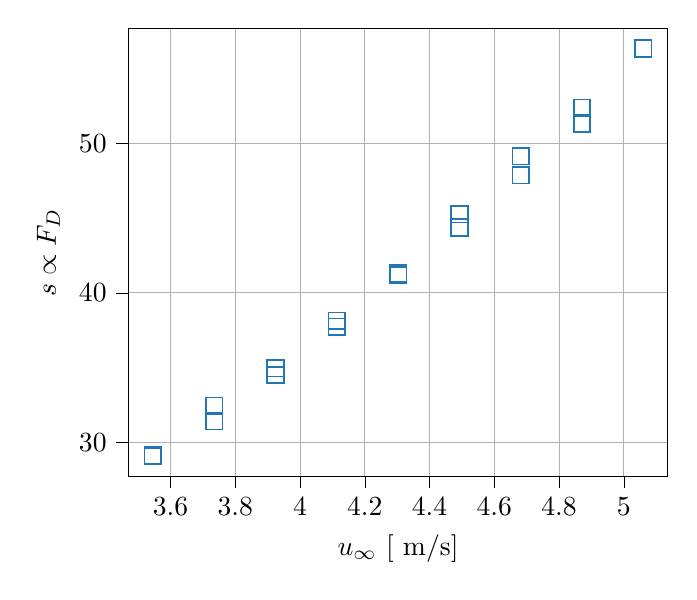
\begin{tikzpicture}

\definecolor{darkgray176}{RGB}{176,176,176}
\definecolor{steelblue31119180}{RGB}{31,119,180}

\begin{axis}[
tick align=outside,
tick pos=left,
x grid style={darkgray176},
xlabel={\(\displaystyle u_\infty\) [ m/s]},
xmajorgrids,
xmin=3.46924, xmax=5.13596,
xtick style={color=black},
y grid style={darkgray176},
ylabel={\(\displaystyle s\propto F_D\)},
ymajorgrids,
ymin=27.7027253333333, ymax=57.7149713333334,
ytick style={color=black}
]
\addplot [semithick, steelblue31119180, mark=square, mark size=3, mark options={solid,fill opacity=0}, only marks]
table {%
3.545 29.0669183333333
3.545 29.1400683333334
3.7344 31.4019583333333
3.7344 32.4280333333335
3.9238 34.4999183333334
3.9238 34.9475883333334
4.1132 37.7284383333333
4.1132 38.1383783333333
4.3026 41.3029733333334
4.3026 41.1816033333333
4.492 45.2667383333333
4.492 44.3826533333333
4.6814 49.1507933333334
4.6814 47.8737983333333
4.8708 52.3913683333334
4.8708 51.3350133333333
5.0602 56.3507783333334
};
\end{axis}

\end{tikzpicture}
}
		\caption{A series of time averaged force measurements for $t=75$, $L=1.50 D$}\label{fig:FD_series_crude}
	\end{figure}
	
		\begin{figure}
		\centering\resizebox{.495\textwidth}{!}{%
			% This file was created with tikzplotlib v0.10.1.
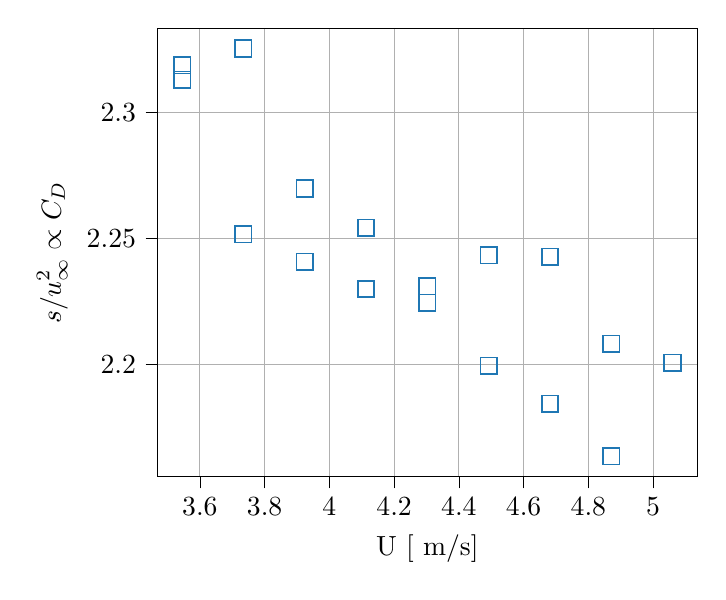
\begin{tikzpicture}

\definecolor{darkgray176}{RGB}{176,176,176}
\definecolor{steelblue31119180}{RGB}{31,119,180}

\begin{axis}[
tick align=outside,
tick pos=left,
x grid style={darkgray176},
xlabel={U [ m/s]},
xmajorgrids,
xmin=3.46924, xmax=5.13596,
xtick style={color=black},
y grid style={darkgray176},
ylabel={\(\displaystyle s/u_\infty^2\propto C_D\)},
ymajorgrids,
ymin=2.15570392000987, ymax=2.33337572573533,
ytick style={color=black}
]
\addplot [semithick, steelblue31119180, mark=square, mark size=3, mark options={solid,fill opacity=0}, only marks]
table {%
3.545 2.31295142114648
3.545 2.31877221007624
3.7344 2.25172352041141
3.7344 2.32529973456599
3.9238 2.240806426426
3.9238 2.26988306954226
4.1132 2.23002214026256
4.1132 2.25425254354886
4.3026 2.23110172074688
4.3026 2.22454556282426
4.492 2.24336380008177
4.492 2.19954963634436
4.6814 2.24274052458761
4.6814 2.18447150710151
4.8708 2.20830546166913
4.8708 2.16377991117921
5.0602 2.20071880479479
};
\end{axis}

\end{tikzpicture}
}
		\caption{$C_D$ estimation for $t=75$, $L=1.50 D$}\label{fig:CD}
	\end{figure}
		\begin{figure}
		\centering\resizebox{.495\textwidth}{!}{%
			% This file was created with tikzplotlib v0.10.1.
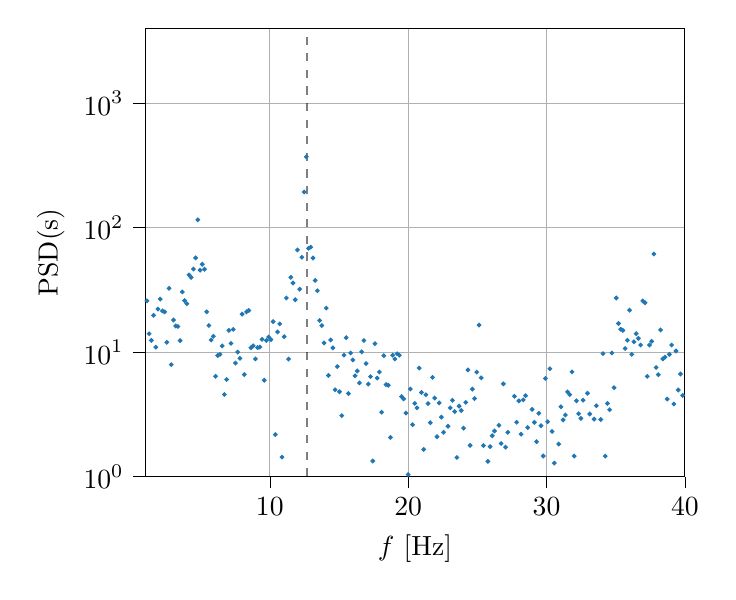
\begin{tikzpicture}

\definecolor{darkgray176}{RGB}{176,176,176}
\definecolor{steelblue31119180}{RGB}{31,119,180}

\begin{axis}[
log basis y={10},
tick align=outside,
tick pos=left,
x grid style={darkgray176},
xlabel={\(\displaystyle f\) [Hz]},
xmajorgrids,
xmin=1, xmax=40,
xtick style={color=black},
y grid style={darkgray176},
ylabel={PSD(s)},
ymajorgrids,
ymin=1, ymax=4000,
ymode=log,
ytick style={color=black},
ytick={0.1,1,10,100,1000,10000,100000},
yticklabels={
  \(\displaystyle {10^{-1}}\),
  \(\displaystyle {10^{0}}\),
  \(\displaystyle {10^{1}}\),
  \(\displaystyle {10^{2}}\),
  \(\displaystyle {10^{3}}\),
  \(\displaystyle {10^{4}}\),
  \(\displaystyle {10^{5}}\)
}
]
\addplot [semithick, black, opacity=0.5, dashed]
table {%
12.67 1
12.67 10000
};
\addplot [semithick, steelblue31119180, mark=*, mark size=0.5, mark options={solid,fill opacity=0}, only marks]
table {%
0 344290.21
0.16 48.5940913085267
0.32 56.1971367097696
0.48 15.6077147591516
0.64 29.4311979231858
0.8 23.0362815057108
0.96 22.700278278816
1.12 25.8051305803003
1.28 14.0450372745
1.44 12.4188302514532
1.6 19.7318406943265
1.76 10.9478715086431
1.92 22.1648695531218
2.08 26.6465341934591
2.24 21.4248481532498
2.4 21.0163906851536
2.56 11.9790060896292
2.72 32.5665081943385
2.88 7.92580206656369
3.04 18.1138838935876
3.2 16.2155281812547
3.36 16.0479205006795
3.52 12.3616521745201
3.68 30.4259600456014
3.84 25.9359606377297
4 24.4866367957159
4.16 41.7444310658014
4.32 39.7714078633993
4.48 46.4717901656709
4.64 57.1519163818526
4.8 115.536146096645
4.96 45.44757234394
5.12 50.7643304386067
5.28 46.2890239323039
5.44 21.0635093016683
5.6 16.3468539720224
5.76 12.5089250835473
5.92 13.376941412296
6.08 6.3843457844401
6.24 9.39367424936799
6.4 9.58068392909324
6.56 11.1953159721502
6.72 4.56248306620644
6.88 6.01606129950114
7.04 14.9378210113762
7.2 11.747437000837
7.36 15.2101304619902
7.52 8.1614441572527
7.68 9.99930543017014
7.84 8.91092145073664
8 20.1903680856275
8.16 6.59665881475255
8.32 21.0725335425008
8.48 21.6086291026822
8.64 10.8350352684488
8.8 11.2327871863153
8.96 8.80868260753813
9.12 10.8688868022202
9.28 10.9784285659797
9.44 12.6647027078595
9.6 5.94307020270513
9.76 12.3979999085702
9.92 13.2023350304577
10.08 12.5761021511854
10.24 17.5643241902043
10.4 2.17493800058064
10.56 14.5148720659837
10.72 16.8529675619441
10.88 1.43132809975182
11.04 13.3022485527137
11.2 27.196423916862
11.36 8.78712152062278
11.52 39.8540450920601
11.68 35.9003916777768
11.84 26.3327803480202
12 66.1364626728467
12.16 32.0069547660638
12.32 57.7625611511697
12.48 193.202096760577
12.64 370.294348459602
12.8 68.1283694420208
12.96 69.7398071102673
13.12 56.988161782859
13.28 37.6434416911302
13.44 31.1196812081898
13.6 17.9514745308772
13.76 16.3240601155071
13.92 11.8387344691216
14.08 22.5599360457472
14.24 6.49005058976226
14.4 12.5154920158426
14.56 10.8144595717371
14.72 4.98007624261662
14.88 7.64354079178726
15.04 4.80138837354472
15.2 3.08570844334166
15.36 9.44907479782403
15.52 13.0510819923792
15.68 4.64271417172965
15.84 9.8257580680866
16 8.64311857362207
16.16 6.44520991364294
16.32 7.04502594021421
16.48 5.65119965428382
16.64 10.0539888888786
16.8 12.3937963301118
16.96 8.08920972353392
17.12 5.53591903268358
17.28 6.35466534423873
17.44 1.33345830054093
17.6 11.6743163156589
17.76 6.1834466510864
17.92 6.92023402405271
18.08 3.28335359159321
18.24 9.35437228725832
18.4 5.48509406340518
18.56 5.41594386912571
18.72 2.06096782726901
18.88 9.43717277889528
19.04 8.80857531582979
19.2 9.69051606015912
19.36 9.44976717461566
19.52 4.39260715824741
19.68 4.20318350809502
19.84 3.23694884781833
20 1.03754517973996
20.16 5.05344294493543
20.32 2.61158416097196
20.48 3.87171069174262
20.64 3.56401039480894
20.8 7.43972914625819
20.96 4.73739695829923
21.12 1.65097473722941
21.28 4.54564660461243
21.44 3.86074656177002
21.6 2.70575174062635
21.76 6.25916987473004
21.92 4.27205730978644
22.08 2.08805170751666
22.24 3.9054225722132
22.4 2.99959063545255
22.56 2.26704277286698
22.72 0.945066329614922
22.88 2.53375286295085
23.04 3.56142314953483
23.2 4.09568711900297
23.36 3.32893630800066
23.52 1.4233420353515
23.68 3.6806136107934
23.84 3.3935920635407
24 2.44618817078043
24.16 3.94304875839636
24.32 7.191492610484
24.48 1.7796365357441
24.64 5.03755345024774
24.8 4.23493214247975
24.96 6.89951393080465
25.12 16.4871692697997
25.28 6.2129658528095
25.44 1.77401868596947
25.6 0.164364359849632
25.76 1.32301221774566
25.92 1.73929313875989
26.08 2.12687735833417
26.24 2.32212323682263
26.4 0.460529734950786
26.56 2.58030756144118
26.72 1.84344422378538
26.88 5.5532650497663
27.04 1.72059019233555
27.2 2.26511724555222
27.36 0.610563968222995
27.52 0.540740578591123
27.68 4.41004502760698
27.84 2.7288484176076
28 4.05225963647022
28.16 2.18895766445607
28.32 4.12986524029211
28.48 4.46303673847434
28.64 2.47509210102526
28.8 0.713288476053831
28.96 3.462537361354
29.12 2.7245310942178
29.28 1.90681120408595
29.44 3.22200202033181
29.6 2.55739801954695
29.76 1.46305380310595
29.92 6.14568354106764
30.08 2.75577356943838
30.24 7.34981829808117
30.4 2.30426116336006
30.56 1.28258607925263
30.72 0.903180857116896
30.88 1.82374844627502
31.04 3.63479147677826
31.2 2.85168707122348
31.36 3.12414843519009
31.52 4.78376517117976
31.68 4.54944944689312
31.84 6.93745299067803
32 1.46071945365437
32.16 4.06186082856019
32.32 3.1987132850464
32.48 2.93283963079869
32.64 4.10699582358499
32.8 0.299999447819194
32.96 4.66966154866397
33.12 3.18159800267383
33.28 0.939710535821062
33.44 2.89306179390201
33.6 3.70813344528552
33.76 0.373522990032993
33.92 2.87185447023436
34.08 9.7081395339159
34.24 1.4594764172418
34.4 3.86870486066935
34.56 3.43721991251264
34.72 9.83317188643172
34.88 5.17638631319406
35.04 27.200882304785
35.2 16.9664638975503
35.36 15.2617696584342
35.52 14.9254088663345
35.68 10.679899865989
35.84 12.4409261094704
36 21.7042879495356
36.16 9.58011060427872
36.32 12.093470867442
36.48 14.0554150669453
36.64 12.8902618817736
36.8 11.3968211876588
36.96 25.7626941851309
37.12 24.9058864806309
37.28 6.37689788965512
37.44 11.4017426502697
37.6 12.1961599178829
37.76 61.4109334225994
37.92 7.52166503840542
38.08 6.58726976091224
38.24 15.059941620024
38.4 8.80902924382398
38.56 9.11181123006144
38.72 4.19666023074703
38.88 9.58392897149165
39.04 11.3870235765177
39.2 3.82592775434443
39.36 10.2019760175514
39.52 4.95945447945237
39.68 6.66275006166158
39.84 4.48506147243625
-40 4.66999999999961
-39.84 4.48506147243626
-39.68 6.66275006166158
-39.52 4.95945447945237
-39.36 10.2019760175514
-39.2 3.82592775434443
-39.04 11.3870235765177
-38.88 9.58392897149166
-38.72 4.19666023074702
-38.56 9.11181123006144
-38.4 8.80902924382398
-38.24 15.059941620024
-38.08 6.58726976091224
-37.92 7.52166503840541
-37.76 61.4109334225994
-37.6 12.1961599178829
-37.44 11.4017426502697
-37.28 6.37689788965512
-37.12 24.9058864806309
-36.96 25.7626941851309
-36.8 11.3968211876588
-36.64 12.8902618817736
-36.48 14.0554150669453
-36.32 12.093470867442
-36.16 9.58011060427872
-36 21.7042879495356
-35.84 12.4409261094704
-35.68 10.679899865989
-35.52 14.9254088663345
-35.36 15.2617696584342
-35.2 16.9664638975503
-35.04 27.200882304785
-34.88 5.17638631319405
-34.72 9.83317188643173
-34.56 3.43721991251263
-34.4 3.86870486066935
-34.24 1.45947641724179
-34.08 9.7081395339159
-33.92 2.87185447023435
-33.76 0.373522990032995
-33.6 3.70813344528552
-33.44 2.89306179390202
-33.28 0.939710535821061
-33.12 3.18159800267382
-32.96 4.66966154866398
-32.8 0.299999447819193
-32.64 4.10699582358499
-32.48 2.93283963079869
-32.32 3.19871328504639
-32.16 4.06186082856021
-32 1.46071945365437
-31.84 6.93745299067805
-31.68 4.54944944689312
-31.52 4.78376517117976
-31.36 3.12414843519009
-31.2 2.85168707122348
-31.04 3.63479147677826
-30.88 1.82374844627502
-30.72 0.903180857116898
-30.56 1.28258607925263
-30.4 2.30426116336005
-30.24 7.34981829808117
-30.08 2.75577356943838
-29.92 6.14568354106764
-29.76 1.46305380310594
-29.6 2.55739801954695
-29.44 3.22200202033181
-29.28 1.90681120408596
-29.12 2.7245310942178
-28.96 3.46253736135399
-28.8 0.713288476053834
-28.64 2.47509210102526
-28.48 4.46303673847435
-28.32 4.1298652402921
-28.16 2.18895766445607
-28 4.05225963647022
-27.84 2.7288484176076
-27.68 4.41004502760699
-27.52 0.540740578591119
-27.36 0.610563968223
-27.2 2.26511724555221
-27.04 1.72059019233555
-26.88 5.5532650497663
-26.72 1.84344422378538
-26.56 2.58030756144118
-26.4 0.460529734950783
-26.24 2.32212323682263
-26.08 2.12687735833416
-25.92 1.73929313875989
-25.76 1.32301221774566
-25.6 0.164364359849632
-25.44 1.77401868596947
-25.28 6.21296585280951
-25.12 16.4871692697997
-24.96 6.89951393080464
-24.8 4.23493214247976
-24.64 5.03755345024774
-24.48 1.7796365357441
-24.32 7.19149261048399
-24.16 3.94304875839637
-24 2.44618817078043
-23.84 3.39359206354071
-23.68 3.68061361079339
-23.52 1.4233420353515
-23.36 3.32893630800066
-23.2 4.09568711900297
-23.04 3.56142314953483
-22.88 2.53375286295084
-22.72 0.945066329614927
-22.56 2.267042772867
-22.4 2.99959063545255
-22.24 3.90542257221322
-22.08 2.08805170751665
-21.92 4.27205730978644
-21.76 6.25916987473004
-21.6 2.70575174062635
-21.44 3.86074656177002
-21.28 4.54564660461242
-21.12 1.65097473722941
-20.96 4.73739695829923
-20.8 7.43972914625818
-20.64 3.56401039480896
-20.48 3.87171069174261
-20.32 2.61158416097196
-20.16 5.05344294493543
-20 1.03754517973996
-19.84 3.23694884781833
-19.68 4.20318350809503
-19.52 4.39260715824745
-19.36 9.44976717461567
-19.2 9.69051606015913
-19.04 8.8085753158298
-18.88 9.43717277889528
-18.72 2.06096782726901
-18.56 5.41594386912571
-18.4 5.48509406340518
-18.24 9.35437228725832
-18.08 3.28335359159321
-17.92 6.92023402405271
-17.76 6.18344665108639
-17.6 11.6743163156589
-17.44 1.33345830054093
-17.28 6.35466534423872
-17.12 5.53591903268358
-16.96 8.08920972353391
-16.8 12.3937963301118
-16.64 10.0539888888786
-16.48 5.65119965428382
-16.32 7.0450259402142
-16.16 6.44520991364295
-16 8.64311857362207
-15.84 9.82575806808662
-15.68 4.64271417172965
-15.52 13.0510819923792
-15.36 9.44907479782403
-15.2 3.08570844334166
-15.04 4.80138837354473
-14.88 7.64354079178726
-14.72 4.98007624261662
-14.56 10.8144595717371
-14.4 12.5154920158426
-14.24 6.49005058976226
-14.08 22.5599360457472
-13.92 11.8387344691216
-13.76 16.3240601155071
-13.6 17.9514745308772
-13.44 31.1196812081897
-13.28 37.6434416911302
-13.12 56.988161782859
-12.96 69.7398071102673
-12.8 68.1283694420208
-12.64 370.294348459602
-12.48 193.202096760577
-12.32 57.7625611511697
-12.16 32.0069547660638
-12 66.1364626728468
-11.84 26.3327803480202
-11.68 35.9003916777768
-11.52 39.8540450920601
-11.36 8.7871215206228
-11.2 27.196423916862
-11.04 13.3022485527137
-10.88 1.43132809975181
-10.72 16.8529675619441
-10.56 14.5148720659837
-10.4 2.17493800058064
-10.24 17.5643241902043
-10.08 12.5761021511854
-9.92 13.2023350304577
-9.76 12.3979999085702
-9.6 5.94307020270513
-9.44 12.6647027078595
-9.28 10.9784285659797
-9.12 10.8688868022202
-8.96 8.80868260753813
-8.8 11.2327871863153
-8.64 10.8350352684488
-8.48 21.6086291026822
-8.32 21.0725335425008
-8.16 6.59665881475255
-8 20.1903680856275
-7.84 8.91092145073664
-7.68 9.99930543017014
-7.52 8.1614441572527
-7.36 15.2101304619902
-7.2 11.7474370008371
-7.04 14.9378210113762
-6.88 6.01606129950114
-6.72 4.56248306620644
-6.56 11.1953159721502
-6.4 9.58068392909324
-6.24 9.39367424936798
-6.08 6.3843457844401
-5.92 13.376941412296
-5.76 12.5089250835473
-5.6 16.3468539720224
-5.44 21.0635093016683
-5.28 46.2890239323039
-5.12 50.7643304386067
-4.96 45.44757234394
-4.8 115.536146096645
-4.64 57.1519163818526
-4.48 46.4717901656709
-4.32 39.7714078633993
-4.16 41.7444310658014
-4 24.4866367957159
-3.84 25.9359606377297
-3.68 30.4259600456014
-3.52 12.3616521745201
-3.36 16.0479205006795
-3.2 16.2155281812547
-3.04 18.1138838935876
-2.88 7.92580206656369
-2.72 32.5665081943385
-2.56 11.9790060896292
-2.4 21.0163906851536
-2.24 21.4248481532498
-2.08 26.6465341934591
-1.92 22.1648695531218
-1.76 10.9478715086431
-1.6 19.7318406943265
-1.44 12.4188302514532
-1.28 14.0450372745
-1.12 25.8051305803003
-0.96 22.700278278816
-0.8 23.0362815057108
-0.64 29.4311979231858
-0.48 15.6077147591516
-0.32 56.1971367097696
-0.16 48.5940913085267
};
\end{axis}

\end{tikzpicture}
}
		\caption{FFT of s. $t=0$, $L=0 D$, $U = 3.5m/s$}\label{fig:FD_fourier}
	\end{figure}
	
			\begin{figure}
		\centering\resizebox{.495\textwidth}{!}{%
			% This file was created with tikzplotlib v0.10.1.
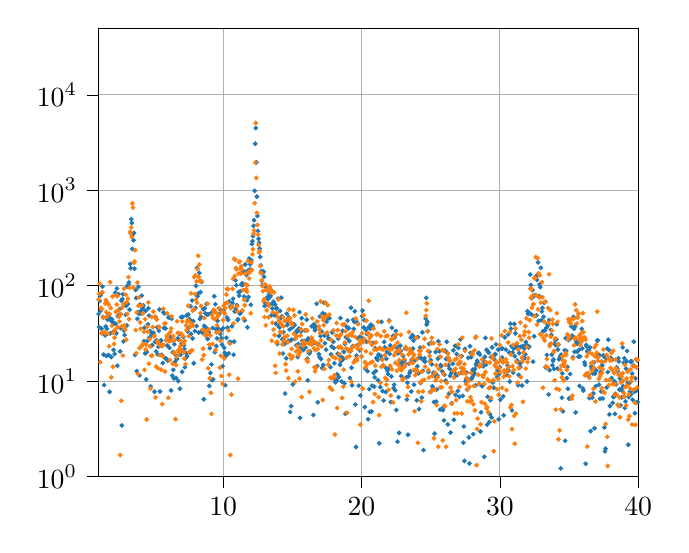
\begin{tikzpicture}

\definecolor{darkgray176}{RGB}{176,176,176}
\definecolor{darkorange25512714}{RGB}{255,127,14}
\definecolor{steelblue31119180}{RGB}{31,119,180}

\begin{axis}[
log basis y={10},
tick align=outside,
tick pos=left,
x grid style={darkgray176},
xmajorgrids,
xmin=1, xmax=40,
xtick style={color=black},
y grid style={darkgray176},
ymajorgrids,
ymin=1, ymax=50000,
ymode=log,
ytick style={color=black},
ytick={0.1,1,10,100,1000,10000,100000,1000000},
yticklabels={
  \(\displaystyle {10^{-1}}\),
  \(\displaystyle {10^{0}}\),
  \(\displaystyle {10^{1}}\),
  \(\displaystyle {10^{2}}\),
  \(\displaystyle {10^{3}}\),
  \(\displaystyle {10^{4}}\),
  \(\displaystyle {10^{5}}\),
  \(\displaystyle {10^{6}}\)
}
]
\addplot [semithick, steelblue31119180, mark=*, mark size=0.5, mark options={solid,fill opacity=0}, only marks]
table {%
0 1636872.8
0.04 101.226909919817
0.08 19.2104729203873
0.12 32.8101240896957
0.16 22.3026463832732
0.2 75.1119321249588
0.24 22.7002628761676
0.28 20.45728939232
0.32 35.9241434549958
0.36 42.077642084534
0.4 36.6359635173614
0.44 43.3550645501975
0.48 17.4076178711499
0.52 45.0114532613196
0.56 10.8115093650946
0.6 33.7661991657396
0.64 0.415479306645896
0.68 19.3151799166577
0.72 25.8140217200713
0.76 52.186824456731
0.8 14.9099375631247
0.84 50.8927385667298
0.88 28.4234382947898
0.92 1.89405578918961
0.96 71.8716292583859
1 50.5212182609094
1.04 36.926458821409
1.08 69.509827025158
1.12 78.6726084008061
1.16 54.9051252588917
1.2 35.5148090951297
1.24 84.1549909330219
1.28 98.0960535754222
1.32 47.1520881445106
1.36 18.9913463316238
1.4 9.10253259981402
1.44 30.7071392461371
1.48 30.2756036885152
1.52 37.4051626866499
1.56 18.3802425154499
1.6 35.4428582759474
1.64 44.2605009223302
1.68 49.3794945925362
1.72 18.7665338798992
1.76 47.0367737510317
1.8 7.72222921354096
1.84 31.6311963803772
1.88 43.0861312251559
1.92 17.8771894081939
1.96 44.4507950790454
2 41.7797921020003
2.04 32.5806708357959
2.08 21.240586771214
2.12 40.4123522749672
2.16 19.2720483502086
2.2 84.4893715894479
2.24 39.9011381956191
2.28 31.7632505964232
2.32 93.4880119111983
2.36 14.4967887427153
2.4 47.9703006871989
2.44 81.6141853875091
2.48 49.6619449695747
2.52 56.9183157203302
2.56 20.4834486288977
2.6 35.9736556971913
2.64 69.6942822401769
2.68 3.43719944657668
2.72 72.5642331745395
2.76 81.4167141594258
2.8 26.099519728549
2.84 33.9063581021424
2.88 30.4402402663239
2.92 64.8235042321557
2.96 49.7972801939804
3 61.4921379670892
3.04 38.3809826460368
3.08 98.0057069835618
3.12 64.6541084758104
3.16 102.945049111525
3.2 108.396558551149
3.24 56.0727785289393
3.28 169.407394191877
3.32 152.802002574489
3.36 498.33342908334
3.4 455.32379738434
3.44 242.917793412258
3.48 346.386067394226
3.52 299.673218302362
3.56 357.688067624931
3.6 150.747315162374
3.64 18.8293485858793
3.68 90.4769459574014
3.72 74.5023592951937
3.76 12.7296268248311
3.8 44.983494747601
3.84 52.546594999426
3.88 97.0527870170446
3.92 50.7143798304692
3.96 11.4897907550501
4 63.314747235585
4.04 54.2407718148583
4.08 51.4232764321927
4.12 78.8631985713012
4.16 59.2683249640642
4.2 56.7843337952617
4.24 62.0730050327365
4.28 26.2139775794192
4.32 36.2570752890959
4.36 19.5271720872096
4.4 54.5194310899326
4.44 10.4305068337464
4.48 20.2104107345986
4.52 26.3640661964945
4.56 39.347497191934
4.6 58.0400683347259
4.64 48.5959123203186
4.68 28.6858796175618
4.72 33.4730603776874
4.76 8.78345634775671
4.8 23.4148948230106
4.84 30.9068660180771
4.88 23.8706510422462
4.92 31.6240133394021
4.96 32.0219902168469
5 30.5093924179447
5.04 7.73905576606335
5.08 25.7316779973825
5.12 46.9788401431333
5.16 20.4539688845351
5.2 26.7846516875473
5.24 36.7278703458419
5.28 19.0782403026291
5.32 22.9561643810778
5.36 33.7442515513825
5.4 56.4063179244564
5.44 7.79391451150776
5.48 26.2096252898971
5.52 26.7549604385958
5.56 18.8511296077554
5.6 23.6526722718085
5.64 15.4841676670862
5.68 52.7004351000856
5.72 36.0324186636286
5.76 51.287828106469
5.8 17.4063182686453
5.84 35.6707322747383
5.88 17.2212431839665
5.92 27.183480478418
5.96 23.6798250935305
6 16.4328465175584
6.04 46.446532511869
6.08 26.6908979022059
6.12 22.3338685197236
6.16 46.7855481210382
6.2 28.907653342334
6.24 7.997913807683
6.28 45.1093555038066
6.32 11.4242866692715
6.36 20.0610049194661
6.4 13.1434435087143
6.44 10.6779064782248
6.48 24.3601438526192
6.52 15.927777801991
6.56 18.8759958369016
6.6 10.7897477607943
6.64 17.1317314209851
6.68 17.1621693820207
6.72 28.0594828721076
6.76 10.0126875725368
6.8 27.2877553965273
6.84 31.2774432138869
6.88 8.32912206719144
6.92 18.9242366603603
6.96 46.9159762750239
7 24.8098237330821
7.04 12.5066030744971
7.08 47.2535490761724
7.12 29.0044696236064
7.16 23.7721976620224
7.2 21.7342456753174
7.24 14.0219044845415
7.28 17.3538398839914
7.32 19.6184329411272
7.36 48.8172489837866
7.4 18.2282365827677
7.44 33.1416053561594
7.48 49.8911259204539
7.52 36.4559498223658
7.56 44.7775251772138
7.6 20.0329718418302
7.64 60.9511153527442
7.68 31.200154434866
7.72 42.2259058124495
7.76 70.0459868994574
7.8 28.0397745624018
7.84 42.4934796481557
7.88 15.4087727781664
7.92 56.684096222745
7.96 33.5181391701103
8 58.5806890055326
8.04 99.9491683081813
8.08 37.7664313304789
8.12 153.58563185445
8.16 77.5836778066495
8.2 83.1640054819167
8.24 32.3326111785922
8.28 136.275880197911
8.32 44.7984807703697
8.36 85.4948697756975
8.4 47.3967051636071
8.44 109.602183225897
8.48 33.4102362822812
8.52 31.9870808673942
8.56 56.6247015397822
8.6 6.46455939911828
8.64 37.8964409045802
8.68 57.9540735146262
8.72 51.4367242343709
8.76 36.4213554669754
8.8 64.4863564670231
8.84 49.8339346739162
8.88 27.735795786074
8.92 50.1138558070514
8.96 32.5945961158851
9 8.90151023876883
9.04 22.1963529591832
9.08 12.1935389417885
9.12 51.4739526227841
9.16 14.9696146698972
9.2 10.2430205538246
9.24 36.0956686244346
9.28 10.4709887157562
9.32 54.720849043741
9.36 77.5727651707129
9.4 20.1003050208814
9.44 63.9619404772004
9.48 34.918381656646
9.52 23.3211096548438
9.56 28.0714937411131
9.6 42.902698173003
9.64 35.7198338763373
9.68 35.0871296369545
9.72 50.4833126116554
9.76 56.9138826429829
9.8 31.2051988023062
9.84 33.5979590272651
9.88 28.2871985418244
9.92 24.1259136737386
9.96 14.3240003478797
10 35.8326314512913
10.04 55.1718875570035
10.08 22.3654523404002
10.12 19.816610098879
10.16 9.058352811756
10.2 18.4309531079389
10.24 28.4544341634766
10.28 46.4095946485539
10.32 36.2826810114419
10.36 43.8906135508261
10.4 19.5079822620486
10.44 68.4976098931806
10.48 25.7390564064528
10.52 60.4207517394052
10.56 25.5297373698633
10.6 58.8643465204234
10.64 37.607075506113
10.68 66.0230681384632
10.72 73.0363189976147
10.76 18.9235166728793
10.8 26.0096598533442
10.84 53.6085597032786
10.88 114.419523036914
10.92 57.3514239770114
10.96 101.217488014156
11 62.7348141185232
11.04 43.6368891178926
11.08 44.558911940837
11.12 85.7655250986241
11.16 78.6663121921234
11.2 51.1536973319595
11.24 87.4195114701234
11.28 51.7376834624114
11.32 102.450647455444
11.36 105.716991963926
11.4 102.39867387359
11.44 142.465877261969
11.48 103.585994333879
11.52 76.9918450935321
11.56 43.3189353516299
11.6 166.940687752473
11.64 139.737015910251
11.68 129.864147387742
11.72 70.4423825784748
11.76 36.6924661504289
11.8 143.950177009077
11.84 76.2956774855685
11.88 192.236745652809
11.92 148.380317801236
11.96 167.220834789787
12 63.1548815668027
12.04 184.93135672656
12.08 273.975638757352
12.12 293.075262096559
12.16 331.154853889782
12.2 424.366101093074
12.24 486.46488159513
12.28 988.397609466294
12.32 3076.43744715352
12.36 4495.3075636971
12.4 1962.99019366755
12.44 859.393445532514
12.48 538.785371814641
12.52 374.175912081874
12.56 310.487021583446
12.6 281.589504730845
12.64 244.75135745832
12.68 200.171244954799
12.72 163.692082097012
12.76 142.332297607079
12.8 112.003045794509
12.84 101.21442527369
12.88 137.58674132828
12.92 141.060919633102
12.96 124.513614480143
13 61.3160267789844
13.04 65.4586022965257
13.08 97.0137171396217
13.12 64.2787163430442
13.16 74.8619743821606
13.2 89.8344031377821
13.24 72.3816344151754
13.28 91.6429376273485
13.32 80.9041680173028
13.36 75.6565542729357
13.4 63.6559953459384
13.44 78.3320535250934
13.48 48.9286026271717
13.52 88.3461977393588
13.56 57.6954025602796
13.6 64.8817068749482
13.64 67.9247490583802
13.68 49.5438799475601
13.72 49.0670081965865
13.76 63.6261146529241
13.8 40.0620089653736
13.84 57.6571013272353
13.88 58.0759879266198
13.92 24.5346921358524
13.96 73.110073183607
14 37.7339937772514
14.04 29.7261065862697
14.08 36.5860664246302
14.12 54.3248164069673
14.16 45.841743671854
14.2 74.7963404110794
14.24 47.6075860050601
14.28 27.4047506428412
14.32 19.4986871817045
14.36 32.5987476709138
14.4 24.4694478606264
14.44 28.6186173027331
14.48 7.42808791759554
14.52 25.1155689434217
14.56 17.37284935018
14.6 50.9105976660549
14.64 38.7213265554112
14.68 41.6784509074622
14.72 26.4659097350139
14.76 46.447307650354
14.8 34.7182500003915
14.84 4.75003948698359
14.88 26.6928498927182
14.92 5.46161858691747
14.96 27.1991237932512
15 36.4137581118843
15.04 9.24072201974628
15.08 38.8151770924782
15.12 39.2968168937758
15.16 38.5680094953707
15.2 27.7321982198324
15.24 31.7412250445286
15.28 23.6584242512962
15.32 33.5359915446628
15.36 33.0556077689989
15.4 17.8954831283582
15.44 24.5224571987837
15.48 35.5569308970087
15.52 52.9630885250437
15.56 4.11279336328503
15.6 22.2752480547774
15.64 33.1514538083204
15.68 45.6523326331731
15.72 26.4576299182834
15.76 24.4694957103566
15.8 21.2301854679541
15.84 25.8533058900797
15.88 26.1876115363047
15.92 33.972374924561
15.96 22.5561302371512
16 26.391293354794
16.04 44.0812122083001
16.08 17.1563022038292
16.12 10.1849761595086
16.16 28.0296893889865
16.2 19.7729331281822
16.24 19.531967853637
16.28 20.416615861815
16.32 26.7345083272519
16.36 28.1133370957785
16.4 37.6276840755591
16.44 26.8613456256098
16.48 24.7739670399819
16.52 4.41500503692398
16.56 39.4481073954873
16.6 36.2601524021475
16.64 34.1364859664606
16.68 25.050991428653
16.72 37.1679360176754
16.76 64.7321770659272
16.8 14.368650571684
16.84 6.00134518261531
16.88 24.4889642050249
16.92 19.1709603619276
16.96 17.8997020781359
17 47.6238968367159
17.04 29.6446108068573
17.08 17.0304538404132
17.12 33.0434173865973
17.16 13.69921605928
17.2 51.4974903835007
17.24 14.7698093499647
17.28 66.3547446174838
17.32 30.0222684750717
17.36 24.9437388523626
17.4 49.5957554902562
17.44 21.3866008101055
17.48 41.8734575035485
17.52 30.4766486199873
17.56 45.7396881976601
17.6 27.9320149695626
17.64 45.9839103663761
17.68 45.6525628231527
17.72 27.573159817327
17.76 14.030840657582
17.8 19.0618802974196
17.84 23.0897826998074
17.88 32.300171322636
17.92 33.1949759751855
17.96 25.8654321522586
18 22.1910137723399
18.04 15.4024669638837
18.08 10.3538332063886
18.12 9.70534283589175
18.16 10.3202495890931
18.2 10.1837086977865
18.24 11.7881424706504
18.28 19.3695507356169
18.32 27.9317749040591
18.36 11.057097939083
18.4 18.5959986676468
18.44 14.8220245289995
18.48 45.7958375328647
18.52 16.1467327885935
18.56 9.9291323235764
18.6 17.7125773307758
18.64 33.7008706332367
18.68 17.0735519104818
18.72 20.2262350460101
18.76 9.46980736062808
18.8 24.5631920631403
18.84 4.5530484804511
18.88 29.0257008091846
18.92 37.2244777174436
18.96 28.2488399431927
19 43.1921637228171
19.04 35.9277056987798
19.08 35.8345394741089
19.12 26.3358165277132
19.16 10.7832868671208
19.2 20.6410568675721
19.24 58.8131430088909
19.28 13.819107013842
19.32 9.04068264081408
19.36 23.1798432284607
19.4 43.9469245439066
19.44 35.1870128592416
19.48 41.7482115810773
19.52 53.9272938178898
19.56 5.69378713000569
19.6 2.04103207332898
19.64 18.5280340386018
19.68 41.4901509197799
19.72 23.9007827412351
19.76 28.0677600013869
19.8 8.97949324757772
19.84 28.9715605068701
19.88 20.9682729339453
19.92 7.07859977857194
19.96 28.6745018947721
20 18.0553039298644
20.04 48.1447684266148
20.08 54.8814724767364
20.12 27.8319264532273
20.16 36.5570011379836
20.2 43.6485632857102
20.24 5.35427215867052
20.28 13.4850993653573
20.32 34.447933856536
20.36 25.8704609896172
20.4 31.1732804112441
20.44 12.73050348605
20.48 3.99000813978374
20.52 36.697984984523
20.56 8.2558867666508
20.6 4.76120976131413
20.64 35.3847193710351
20.68 39.1490341587128
20.72 4.80548079527801
20.76 8.98135110490695
20.8 37.5463486048131
20.84 25.0851709287447
20.88 12.1875648796278
20.92 8.74172885628185
20.96 10.9613170927173
21 22.1693181443099
21.04 12.7802811928282
21.08 17.4259242746118
21.12 17.5940129569097
21.16 16.6763915552821
21.2 10.2342287527935
21.24 19.0155195946741
21.28 2.23085608344153
21.32 22.2088329053053
21.36 8.66849182467112
21.4 18.3678927506818
21.44 41.8139763871847
21.48 17.0394545732069
21.52 7.86986624115954
21.56 14.6780446124881
21.6 6.2728526823416
21.64 25.7385782072667
21.68 22.5208195972301
21.72 13.9422180622704
21.76 7.68443172908694
21.8 17.1531273851135
21.84 20.3171682068373
21.88 12.9369670625307
21.92 11.8712008028035
21.96 13.6628099042899
22 43.0799504236273
22.04 19.3153856472946
22.08 23.698688895761
22.12 6.03955094590257
22.16 11.1677320831243
22.2 36.2548723543853
22.24 27.7818488286002
22.28 29.891200810663
22.32 8.45538611664386
22.36 9.16959592691265
22.4 28.5756468660431
22.44 8.00676813478048
22.48 33.4915198243548
22.52 4.98658700102241
22.56 22.4924804440994
22.6 2.32221533626814
22.64 19.5836112615879
22.68 6.78607110255931
22.72 2.87054020049125
22.76 15.1777032254494
22.8 23.4908437483458
22.84 20.8578035624207
22.88 11.2804011387105
22.92 15.7996342519396
22.96 13.8286160291286
23 18.3237074664756
23.04 14.4184125327479
23.08 14.9856594982144
23.12 16.5573718776799
23.16 22.0309708364299
23.2 15.086453379153
23.24 10.9737305736836
23.28 6.42094411887483
23.32 9.59271704075113
23.36 2.74043871221817
23.4 11.2276322814955
23.44 15.2387318706461
23.48 12.0836808599137
23.52 12.6883893235024
23.56 28.572009522017
23.6 7.77812606278207
23.64 16.6840561793024
23.68 30.3068930375578
23.72 21.9569513125284
23.76 26.5893571404182
23.8 9.17026249980709
23.84 28.5958068385147
23.88 16.5585880084024
23.92 12.9416254029562
23.96 13.205727963359
24 6.29335964622882
24.04 14.2829907230381
24.08 28.9223358131945
24.12 12.0724910404147
24.16 5.10432215135909
24.2 17.8574282396768
24.24 22.5154993563516
24.28 9.57796179213686
24.32 17.3691838805965
24.36 6.70632662762024
24.4 32.4716572657713
24.44 12.792419476341
24.48 1.89059895883263
24.52 16.3367698124194
24.56 17.3337111542037
24.6 16.0249786375114
24.64 45.2519209447812
24.68 74.6245814068681
24.72 39.2356754932626
24.76 41.7821041291745
24.8 33.3226211489399
24.84 12.4952590483864
24.88 24.5467430032009
24.92 20.3009825603291
24.96 7.69712236112342
25 16.5838597294914
25.04 25.3322606639444
25.08 15.0377673517916
25.12 8.84308465087741
25.16 8.40805893157565
25.2 12.2528831301072
25.24 6.04121681729331
25.28 2.82202068769645
25.32 11.1751460242939
25.36 20.2181086254409
25.4 6.08862528814112
25.44 8.17892506333228
25.48 11.4389147157573
25.52 17.1504941293824
25.56 26.1076088212423
25.6 17.7379335249217
25.64 20.4982396555307
25.68 5.03445232731005
25.72 14.7076935512371
25.76 14.3340927409627
25.8 0.776656976696651
25.84 12.6592140173902
25.88 4.96138505076775
25.92 5.31024543937209
25.96 3.88002198099685
26 11.6991476453982
26.04 20.9832934577901
26.08 10.1637762568967
26.12 17.1200803348716
26.16 25.8509571250947
26.2 19.7042501020987
26.24 3.51855254421561
26.28 14.6359217245905
26.32 7.38946567854519
26.36 13.535821293091
26.4 11.352358908998
26.44 2.89093416671811
26.48 12.1187026191566
26.52 5.87443224678625
26.56 12.7318574720416
26.6 15.1796934754701
26.64 21.0094698511355
26.68 3.93173354678423
26.72 12.3548794096074
26.76 23.4632626199922
26.8 7.16710963229134
26.84 11.6301987070771
26.88 19.1995427049844
26.92 11.5636237380502
26.96 7.86830688811833
27 22.2780274588605
27.04 15.2922944850542
27.08 6.85354954607164
27.12 15.7218081607127
27.16 27.4092463235769
27.2 12.1984011418429
27.24 18.26339553571
27.28 13.619796521464
27.32 7.00980558518909
27.36 2.26414072161991
27.4 3.34363908631006
27.44 1.45870820008196
27.48 21.7287371865894
27.52 9.93720576404315
27.56 10.5568426446978
27.6 12.2669963790352
27.64 8.16852172758718
27.68 10.252348369278
27.72 17.5443825516521
27.76 2.57210201698401
27.8 1.37229452274528
27.84 23.2215172423628
27.88 19.7500060319332
27.92 17.8498015786693
27.96 10.6399402935686
28 11.0162197886829
28.04 13.1832753911828
28.08 2.78483394657623
28.12 11.7762360559317
28.16 12.2296183697814
28.2 13.425000420159
28.24 9.02640575428607
28.28 14.7917245112321
28.32 15.4255831847875
28.36 16.3435696991393
28.4 15.6928836861945
28.44 19.5758219616367
28.48 19.7898554725661
28.52 9.34010788098004
28.56 19.0086920249487
28.6 2.96896459597492
28.64 4.70967040963367
28.68 14.6669701859262
28.72 8.85183355831145
28.76 16.8780977675322
28.8 14.2748133003833
28.84 16.0262827139791
28.88 1.61051955643632
28.92 17.9926303388417
28.96 28.3853140886409
29 14.8860806930287
29.04 21.3121416536051
29.08 3.49590077122385
29.12 6.84675201984848
29.16 20.0792810251964
29.2 19.9892697151909
29.24 3.72210266275558
29.28 4.50597130861019
29.32 6.31524458428312
29.36 17.9233664769261
29.4 4.16734121949779
29.44 22.5679722373045
29.48 9.65899544058392
29.52 10.2499352117369
29.56 8.52779325929991
29.6 16.9616526253665
29.64 18.9730756801473
29.68 19.2443093092625
29.72 24.2928787856372
29.76 13.9402706371696
29.8 11.0057236315757
29.84 12.9880257683342
29.88 21.4550694042628
29.92 3.98741162975537
29.96 11.9072408403201
30 14.0267360164817
30.04 6.38903028180612
30.08 16.7581708010031
30.12 21.7899143334655
30.16 17.6668122352074
30.2 21.9757528780769
30.24 6.91738415872934
30.28 4.38375982630012
30.32 0.134830075514048
30.36 28.7715527478489
30.4 12.4881804518082
30.44 21.3965362345255
30.48 11.6681284426602
30.52 12.9828804810806
30.56 14.6148475283389
30.6 30.8975915398944
30.64 12.8750829882575
30.68 19.9488104041786
30.72 9.89347734608451
30.76 39.9911679755311
30.8 35.4828356888615
30.84 23.2528454857027
30.88 4.94062629340822
30.92 19.92464311305
30.96 12.3019413005809
31 22.0073812896346
31.04 39.6834239274461
31.08 18.2578757402606
31.12 31.6941562380622
31.16 23.8159692128062
31.2 22.4315959950755
31.24 16.4328910421546
31.28 23.1486599058262
31.32 9.08478140837177
31.36 11.6149910779301
31.4 19.6283672135837
31.44 15.256210435812
31.48 14.0544740755038
31.52 22.9142912911407
31.56 15.715481939442
31.6 8.99355588523845
31.64 17.5096685093607
31.68 23.323206748268
31.72 17.4309590177011
31.76 21.9153937542012
31.8 17.4041318690151
31.84 19.0937361034977
31.88 25.6283914486111
31.92 24.0229249077787
31.96 9.91502116871296
32 54.0389409136224
32.04 50.6039874091857
32.08 22.5601238438332
32.12 23.0487358137648
32.16 51.6625465896548
32.2 130.970711690449
32.24 101.585369436903
32.28 73.9340790387513
32.32 49.4565624260149
32.36 90.2814659078473
32.4 15.9869325480664
32.44 77.2872951780701
32.48 29.4865705498206
32.52 79.5084019372552
32.56 123.53184923606
32.6 122.760843956743
32.64 48.8899914709266
32.68 115.266308014697
32.72 130.481585749868
32.76 175.256435837301
32.8 42.7637623645288
32.84 77.8425081738753
32.88 103.773992612674
32.92 96.6125492912846
32.96 154.09708844267
33 43.4906706996915
33.04 53.6875544431275
33.08 58.5276385682781
33.12 33.4610637452266
33.16 47.1937672047174
33.2 66.3559623086588
33.24 33.8598468788102
33.28 67.8957581400236
33.32 13.8416089964239
33.36 36.2123236390229
33.4 18.8028485045142
33.44 39.6016281543035
33.48 38.5737809858026
33.52 7.24349668597569
33.56 43.6995056800671
33.6 13.0297512440813
33.64 24.4213568039782
33.68 34.4496325632655
33.72 30.5157414223448
33.76 18.9672825625733
33.8 14.635160983198
33.84 16.3162531950961
33.88 16.9073858453054
33.92 13.404159240683
33.96 24.6040550239242
34 26.8959506033726
34.04 23.8080539339715
34.08 27.458229179902
34.12 39.4453289352729
34.16 13.5546134645621
34.2 21.4246368021975
34.24 24.1976836258009
34.28 16.9386090335003
34.32 17.3519277310117
34.36 18.1087413400135
34.4 1.21744786635873
34.44 18.9378952076696
34.48 6.70387233103269
34.52 12.0301117783761
34.56 4.82078248423737
34.6 14.6226448846985
34.64 15.5656298822216
34.68 21.0931687773755
34.72 2.37189280075136
34.76 28.1768494226851
34.8 20.7734338655365
34.84 10.7565210164629
34.88 14.0926866567696
34.92 8.31819115801861
34.96 26.9581854128143
35 6.54635707319931
35.04 6.60161797180645
35.08 11.883392324815
35.12 28.2712613791881
35.16 37.495378958543
35.2 29.8860990197494
35.24 29.7187950436367
35.28 17.8022098740583
35.32 47.0310699877638
35.36 35.4620981066115
35.4 20.2829098951114
35.44 37.504561528753
35.48 4.69529390423473
35.52 26.0277653456934
35.56 24.6850900554149
35.6 20.3634818247511
35.64 24.7242627491577
35.68 18.0510894301978
35.72 21.270842117464
35.76 8.91206293969502
35.8 18.1529138748094
35.84 25.5159550931047
35.88 26.2665823513027
35.92 35.2977296139382
35.96 21.9427571398997
36 8.34443637074581
36.04 7.94956633829739
36.08 28.5183020110191
36.12 15.7061333924023
36.16 14.8295366426639
36.2 1.36057221200791
36.24 23.9652814844974
36.28 23.0048594885784
36.32 20.6516295883893
36.36 20.1330818256058
36.4 11.4310566563186
36.44 20.9083404602853
36.48 6.65543867872019
36.52 22.5790349370535
36.56 2.99286991810308
36.6 14.2617593559713
36.64 13.4346570222791
36.68 6.71994663326064
36.72 12.0659187670625
36.76 7.44037655046894
36.8 15.7106669373107
36.84 3.20792230420387
36.88 12.013048701087
36.92 8.82911746543632
36.96 12.9462322096139
37 18.2689890194203
37.04 26.5556002871039
37.08 26.8924580584538
37.12 18.8371391408414
37.16 9.17851326866568
37.2 18.7262786432634
37.24 6.52985412371606
37.28 12.4551383546778
37.32 7.78202075995876
37.36 16.0284220783376
37.4 14.6921491475521
37.44 6.58286450807932
37.48 18.7030175253146
37.52 18.1236397631145
37.56 3.26924636822082
37.6 1.83815799196159
37.64 1.95856623604269
37.68 17.3300743745011
37.72 8.56499650350076
37.76 21.9143917891379
37.8 12.4581707489693
37.84 27.1936633392479
37.88 21.242173134826
37.92 4.47750953099155
37.96 5.4931395126532
38 17.4986858257413
38.04 17.318626243603
38.08 10.7581430981492
38.12 16.7444895637591
38.16 5.91279574392201
38.2 6.85368865010546
38.24 6.83578513448893
38.28 9.95530281295659
38.32 4.53127889853458
38.36 7.3351596050726
38.4 9.24948061736223
38.44 13.9787905638642
38.48 13.5098486686314
38.52 12.7025731219136
38.56 17.3366499335166
38.6 16.0716008382701
38.64 8.14825136333992
38.68 10.6543405730997
38.72 5.56560775681198
38.76 8.26203952685755
38.8 6.76650179535586
38.84 7.91468221003892
38.88 22.6070126476409
38.92 8.84502414769734
38.96 15.6155505269041
39 17.3737324420211
39.04 5.24311294068115
39.08 6.1395591466581
39.12 13.5230017369888
39.16 16.0994929043751
39.2 20.6926730103457
39.24 9.55814299147416
39.28 2.15467060069722
39.32 6.81354813566989
39.36 9.57255880423117
39.4 7.75787998444259
39.44 15.9541430133076
39.48 7.28997723160461
39.52 16.173012967136
39.56 11.9730637249412
39.6 6.37634915473595
39.64 14.5804571924173
39.68 25.8953262702302
39.72 7.739341667348
39.76 4.61395878569266
39.8 10.6997957297636
39.84 5.9930781022364
39.88 7.97701185765969
39.92 16.4313953393853
39.96 6.03664305497599
-40 3.80000000000018
-39.96 6.036643054976
-39.92 16.4313953393854
-39.88 7.97701185765967
-39.84 5.99307810223641
-39.8 10.6997957297637
-39.76 4.61395878569266
-39.72 7.73934166734797
-39.68 25.8953262702302
-39.64 14.5804571924173
-39.6 6.37634915473592
-39.56 11.9730637249412
-39.52 16.173012967136
-39.48 7.28997723160459
-39.44 15.9541430133077
-39.4 7.75787998444257
-39.36 9.57255880423116
-39.32 6.81354813566989
-39.28 2.15467060069717
-39.24 9.55814299147402
-39.2 20.6926730103457
-39.16 16.0994929043751
-39.12 13.5230017369888
-39.08 6.13955914665806
-39.04 5.24311294068116
-39 17.373732442021
-38.96 15.6155505269041
-38.92 8.84502414769743
-38.88 22.6070126476408
-38.84 7.91468221003875
-38.8 6.76650179535576
-38.76 8.2620395268575
-38.72 5.56560775681198
-38.68 10.6543405730997
-38.64 8.14825136333994
-38.6 16.0716008382699
-38.56 17.3366499335165
-38.52 12.7025731219137
-38.48 13.5098486686314
-38.44 13.9787905638642
-38.4 9.24948061736224
-38.36 7.33515960507258
-38.32 4.53127889853459
-38.28 9.95530281295659
-38.24 6.83578513448891
-38.2 6.85368865010547
-38.16 5.912795743922
-38.12 16.7444895637591
-38.08 10.7581430981492
-38.04 17.3186262436031
-38 17.4986858257413
-37.96 5.49313951265319
-37.92 4.47750953099163
-37.88 21.242173134826
-37.84 27.1936633392479
-37.8 12.4581707489694
-37.76 21.9143917891379
-37.72 8.56499650350077
-37.68 17.3300743745012
-37.64 1.95856623604265
-37.6 1.8381579919616
-37.56 3.26924636822094
-37.52 18.1236397631145
-37.48 18.7030175253146
-37.44 6.58286450807932
-37.4 14.6921491475521
-37.36 16.0284220783376
-37.32 7.78202075995886
-37.28 12.4551383546778
-37.24 6.52985412371607
-37.2 18.7262786432634
-37.16 9.17851326866568
-37.12 18.8371391408414
-37.08 26.8924580584538
-37.04 26.5556002871039
-37 18.2689890194203
-36.96 12.9462322096139
-36.92 8.82911746543632
-36.88 12.013048701087
-36.84 3.20792230420383
-36.8 15.7106669373107
-36.76 7.44037655046895
-36.72 12.0659187670625
-36.68 6.71994663326066
-36.64 13.4346570222791
-36.6 14.2617593559712
-36.56 2.99286991810308
-36.52 22.5790349370535
-36.48 6.65543867872019
-36.44 20.9083404602853
-36.4 11.4310566563186
-36.36 20.1330818256058
-36.32 20.6516295883893
-36.28 23.0048594885785
-36.24 23.9652814844973
-36.2 1.36057221200793
-36.16 14.8295366426639
-36.12 15.7061333924023
-36.08 28.5183020110191
-36.04 7.9495663382974
-36 8.34443637074583
-35.96 21.9427571398998
-35.92 35.2977296139383
-35.88 26.2665823513027
-35.84 25.5159550931047
-35.8 18.1529138748093
-35.76 8.91206293969501
-35.72 21.270842117464
-35.68 18.0510894301978
-35.64 24.7242627491575
-35.6 20.3634818247512
-35.56 24.6850900554149
-35.52 26.0277653456934
-35.48 4.69529390423481
-35.44 37.5045615287531
-35.4 20.2829098951114
-35.36 35.4620981066116
-35.32 47.0310699877638
-35.28 17.8022098740583
-35.24 29.7187950436367
-35.2 29.8860990197494
-35.16 37.495378958543
-35.12 28.271261379188
-35.08 11.883392324815
-35.04 6.6016179718064
-35 6.54635707319934
-34.96 26.9581854128142
-34.92 8.31819115801862
-34.88 14.0926866567697
-34.84 10.7565210164629
-34.8 20.7734338655365
-34.76 28.1768494226851
-34.72 2.37189280075125
-34.68 21.0931687773755
-34.64 15.5656298822216
-34.6 14.6226448846985
-34.56 4.82078248423735
-34.52 12.0301117783761
-34.48 6.70387233103269
-34.44 18.9378952076696
-34.4 1.21744786635878
-34.36 18.1087413400135
-34.32 17.3519277310118
-34.28 16.9386090335003
-34.24 24.1976836258009
-34.2 21.4246368021975
-34.16 13.5546134645621
-34.12 39.4453289352729
-34.08 27.458229179902
-34.04 23.8080539339715
-34 26.8959506033726
-33.96 24.6040550239242
-33.92 13.404159240683
-33.88 16.9073858453054
-33.84 16.3162531950962
-33.8 14.635160983198
-33.76 18.9672825625733
-33.72 30.5157414223448
-33.68 34.4496325632655
-33.64 24.4213568039782
-33.6 13.0297512440813
-33.56 43.6995056800671
-33.52 7.24349668597569
-33.48 38.5737809858026
-33.44 39.6016281543034
-33.4 18.8028485045142
-33.36 36.2123236390229
-33.32 13.8416089964239
-33.28 67.8957581400236
-33.24 33.8598468788102
-33.2 66.3559623086588
-33.16 47.1937672047174
-33.12 33.4610637452267
-33.08 58.5276385682781
-33.04 53.6875544431274
-33 43.4906706996916
-32.96 154.09708844267
-32.92 96.6125492912846
-32.88 103.773992612674
-32.84 77.8425081738753
-32.8 42.7637623645287
-32.76 175.256435837301
-32.72 130.481585749868
-32.68 115.266308014697
-32.64 48.8899914709267
-32.6 122.760843956743
-32.56 123.53184923606
-32.52 79.5084019372553
-32.48 29.4865705498207
-32.44 77.28729517807
-32.4 15.9869325480664
-32.36 90.2814659078473
-32.32 49.4565624260149
-32.28 73.9340790387512
-32.24 101.585369436903
-32.2 130.970711690449
-32.16 51.6625465896548
-32.12 23.0487358137647
-32.08 22.5601238438332
-32.04 50.6039874091857
-32 54.0389409136224
-31.96 9.91502116871295
-31.92 24.0229249077787
-31.88 25.6283914486111
-31.84 19.0937361034977
-31.8 17.4041318690151
-31.76 21.9153937542012
-31.72 17.4309590177011
-31.68 23.3232067482681
-31.64 17.5096685093607
-31.6 8.99355588523831
-31.56 15.7154819394419
-31.52 22.9142912911406
-31.48 14.0544740755038
-31.44 15.256210435812
-31.4 19.6283672135838
-31.36 11.6149910779301
-31.32 9.08478140837179
-31.28 23.1486599058262
-31.24 16.4328910421547
-31.2 22.4315959950756
-31.16 23.8159692128062
-31.12 31.6941562380622
-31.08 18.2578757402606
-31.04 39.6834239274461
-31 22.0073812896346
-30.96 12.3019413005809
-30.92 19.92464311305
-30.88 4.94062629340822
-30.84 23.2528454857027
-30.8 35.4828356888615
-30.76 39.9911679755311
-30.72 9.89347734608451
-30.68 19.9488104041786
-30.64 12.8750829882575
-30.6 30.8975915398944
-30.56 14.614847528339
-30.52 12.9828804810807
-30.48 11.6681284426603
-30.44 21.3965362345255
-30.4 12.4881804518082
-30.36 28.7715527478489
-30.32 0.134830075514047
-30.28 4.38375982630016
-30.24 6.9173841587294
-30.2 21.9757528780769
-30.16 17.6668122352073
-30.12 21.7899143334655
-30.08 16.7581708010031
-30.04 6.38903028180611
-30 14.0267360164817
-29.96 11.90724084032
-29.92 3.98741162975539
-29.88 21.4550694042628
-29.84 12.9880257683341
-29.8 11.0057236315757
-29.76 13.9402706371696
-29.72 24.2928787856372
-29.68 19.2443093092625
-29.64 18.9730756801473
-29.6 16.9616526253665
-29.56 8.52779325929985
-29.52 10.2499352117369
-29.48 9.65899544058393
-29.44 22.5679722373045
-29.4 4.16734121949781
-29.36 17.9233664769261
-29.32 6.31524458428316
-29.28 4.50597130861017
-29.24 3.72210266275551
-29.2 19.989269715191
-29.16 20.0792810251963
-29.12 6.84675201984849
-29.08 3.49590077122387
-29.04 21.312141653605
-29 14.8860806930286
-28.96 28.3853140886409
-28.92 17.9926303388417
-28.88 1.61051955643632
-28.84 16.0262827139791
-28.8 14.2748133003833
-28.76 16.8780977675322
-28.72 8.85183355831146
-28.68 14.6669701859262
-28.64 4.70967040963368
-28.6 2.96896459597488
-28.56 19.0086920249487
-28.52 9.34010788098002
-28.48 19.7898554725661
-28.44 19.5758219616367
-28.4 15.6928836861946
-28.36 16.3435696991395
-28.32 15.4255831847872
-28.28 14.7917245112321
-28.24 9.02640575428611
-28.2 13.425000420159
-28.16 12.2296183697814
-28.12 11.7762360559317
-28.08 2.78483394657621
-28.04 13.1832753911829
-28 11.0162197886829
-27.96 10.6399402935686
-27.92 17.8498015786693
-27.88 19.7500060319332
-27.84 23.2215172423629
-27.8 1.37229452274528
-27.76 2.57210201698398
-27.72 17.544382551652
-27.68 10.252348369278
-27.64 8.16852172758712
-27.6 12.2669963790352
-27.56 10.5568426446979
-27.52 9.93720576404314
-27.48 21.7287371865894
-27.44 1.45870820008197
-27.4 3.34363908631008
-27.36 2.26414072161991
-27.32 7.00980558518918
-27.28 13.619796521464
-27.24 18.2633955357099
-27.2 12.1984011418429
-27.16 27.4092463235769
-27.12 15.7218081607127
-27.08 6.85354954607171
-27.04 15.2922944850542
-27 22.2780274588605
-26.96 7.86830688811831
-26.92 11.5636237380502
-26.88 19.1995427049844
-26.84 11.6301987070771
-26.8 7.16710963229135
-26.76 23.4632626199922
-26.72 12.3548794096074
-26.68 3.93173354678438
-26.64 21.0094698511355
-26.6 15.17969347547
-26.56 12.7318574720416
-26.52 5.87443224678627
-26.48 12.1187026191566
-26.44 2.89093416671804
-26.4 11.3523589089979
-26.36 13.535821293091
-26.32 7.38946567854519
-26.28 14.6359217245906
-26.24 3.51855254421562
-26.2 19.7042501020987
-26.16 25.8509571250947
-26.12 17.1200803348715
-26.08 10.1637762568968
-26.04 20.9832934577901
-26 11.6991476453982
-25.96 3.88002198099683
-25.92 5.31024543937211
-25.88 4.96138505076775
-25.84 12.6592140173902
-25.8 0.776656976696586
-25.76 14.3340927409627
-25.72 14.7076935512371
-25.68 5.03445232731006
-25.64 20.4982396555307
-25.6 17.7379335249217
-25.56 26.1076088212424
-25.52 17.1504941293825
-25.48 11.4389147157573
-25.44 8.17892506333229
-25.4 6.08862528814115
-25.36 20.2181086254409
-25.32 11.1751460242939
-25.28 2.82202068769646
-25.24 6.04121681729336
-25.2 12.2528831301072
-25.16 8.40805893157572
-25.12 8.84308465087737
-25.08 15.0377673517916
-25.04 25.3322606639444
-25 16.5838597294914
-24.96 7.69712236112342
-24.92 20.3009825603291
-24.88 24.5467430032009
-24.84 12.4952590483864
-24.8 33.3226211489399
-24.76 41.7821041291745
-24.72 39.2356754932626
-24.68 74.6245814068681
-24.64 45.2519209447812
-24.6 16.0249786375114
-24.56 17.3337111542037
-24.52 16.3367698124194
-24.48 1.89059895883261
-24.44 12.792419476341
-24.4 32.4716572657713
-24.36 6.70632662762026
-24.32 17.3691838805965
-24.28 9.57796179213685
-24.24 22.5154993563516
-24.2 17.8574282396768
-24.16 5.10432215135905
-24.12 12.0724910404146
-24.08 28.9223358131945
-24.04 14.2829907230381
-24 6.29335964622881
-23.96 13.205727963359
-23.92 12.9416254029562
-23.88 16.5585880084024
-23.84 28.5958068385147
-23.8 9.1702624998071
-23.76 26.5893571404182
-23.72 21.9569513125284
-23.68 30.3068930375578
-23.64 16.6840561793024
-23.6 7.77812606278207
-23.56 28.572009522017
-23.52 12.6883893235023
-23.48 12.0836808599137
-23.44 15.2387318706462
-23.4 11.2276322814955
-23.36 2.74043871221816
-23.32 9.59271704075115
-23.28 6.42094411887483
-23.24 10.9737305736836
-23.2 15.086453379153
-23.16 22.0309708364299
-23.12 16.5573718776799
-23.08 14.9856594982145
-23.04 14.418412532748
-23 18.3237074664756
-22.96 13.8286160291286
-22.92 15.7996342519396
-22.88 11.2804011387104
-22.84 20.8578035624207
-22.8 23.4908437483458
-22.76 15.1777032254494
-22.72 2.87054020049126
-22.68 6.78607110255934
-22.64 19.5836112615879
-22.6 2.32221533626811
-22.56 22.4924804440994
-22.52 4.98658700102239
-22.48 33.4915198243548
-22.44 8.00676813478048
-22.4 28.5756468660431
-22.36 9.16959592691266
-22.32 8.45538611664387
-22.28 29.891200810663
-22.24 27.7818488286002
-22.2 36.2548723543853
-22.16 11.1677320831243
-22.12 6.03955094590254
-22.08 23.6986888957611
-22.04 19.3153856472946
-22 43.0799504236273
-21.96 13.66280990429
-21.92 11.8712008028034
-21.88 12.9369670625307
-21.84 20.3171682068373
-21.8 17.1531273851135
-21.76 7.68443172908694
-21.72 13.9422180622704
-21.68 22.5208195972301
-21.64 25.7385782072667
-21.6 6.27285268234158
-21.56 14.678044612488
-21.52 7.86986624115949
-21.48 17.0394545732069
-21.44 41.8139763871846
-21.4 18.3678927506818
-21.36 8.66849182467112
-21.32 22.2088329053054
-21.28 2.23085608344154
-21.24 19.0155195946741
-21.2 10.2342287527935
-21.16 16.6763915552821
-21.12 17.5940129569097
-21.08 17.4259242746118
-21.04 12.7802811928282
-21 22.1693181443099
-20.96 10.9613170927173
-20.92 8.74172885628195
-20.88 12.1875648796278
-20.84 25.0851709287447
-20.8 37.5463486048131
-20.76 8.98135110490696
-20.72 4.805480795278
-20.68 39.1490341587128
-20.64 35.3847193710351
-20.6 4.76120976131417
-20.56 8.25588676665079
-20.52 36.697984984523
-20.48 3.99000813978373
-20.44 12.7305034860501
-20.4 31.1732804112441
-20.36 25.8704609896172
-20.32 34.4479338565361
-20.28 13.4850993653573
-20.24 5.35427215867054
-20.2 43.6485632857102
-20.16 36.5570011379836
-20.12 27.8319264532273
-20.08 54.8814724767364
-20.04 48.1447684266148
-20 18.0553039298643
-19.96 28.6745018947721
-19.92 7.07859977857192
-19.88 20.9682729339453
-19.84 28.9715605068701
-19.8 8.97949324757771
-19.76 28.0677600013869
-19.72 23.900782741235
-19.68 41.4901509197799
-19.64 18.528034038602
-19.6 2.04103207332931
-19.56 5.69378713000571
-19.52 53.9272938178899
-19.48 41.7482115810773
-19.44 35.1870128592416
-19.4 43.9469245439067
-19.36 23.1798432284608
-19.32 9.04068264081404
-19.28 13.819107013842
-19.24 58.8131430088909
-19.2 20.6410568675721
-19.16 10.7832868671208
-19.12 26.3358165277132
-19.08 35.8345394741089
-19.04 35.9277056987798
-19 43.1921637228171
-18.96 28.2488399431928
-18.92 37.2244777174436
-18.88 29.0257008091846
-18.84 4.55304848045112
-18.8 24.5631920631403
-18.76 9.46980736062808
-18.72 20.2262350460102
-18.68 17.0735519104818
-18.64 33.7008706332367
-18.6 17.7125773307758
-18.56 9.9291323235764
-18.52 16.1467327885935
-18.48 45.7958375328647
-18.44 14.8220245289995
-18.4 18.5959986676467
-18.36 11.0570979390831
-18.32 27.9317749040591
-18.28 19.3695507356169
-18.24 11.7881424706504
-18.2 10.1837086977865
-18.16 10.3202495890931
-18.12 9.70534283589183
-18.08 10.3538332063886
-18.04 15.4024669638837
-18 22.1910137723399
-17.96 25.8654321522586
-17.92 33.1949759751855
-17.88 32.300171322636
-17.84 23.0897826998074
-17.8 19.0618802974196
-17.76 14.030840657582
-17.72 27.573159817327
-17.68 45.6525628231527
-17.64 45.9839103663761
-17.6 27.9320149695626
-17.56 45.7396881976601
-17.52 30.4766486199873
-17.48 41.8734575035485
-17.44 21.3866008101055
-17.4 49.5957554902562
-17.36 24.9437388523626
-17.32 30.0222684750717
-17.28 66.3547446174839
-17.24 14.7698093499647
-17.2 51.4974903835007
-17.16 13.69921605928
-17.12 33.0434173865973
-17.08 17.0304538404132
-17.04 29.6446108068573
-17 47.6238968367159
-16.96 17.8997020781359
-16.92 19.1709603619276
-16.88 24.4889642050249
-16.84 6.00134518261521
-16.8 14.368650571684
-16.76 64.7321770659272
-16.72 37.1679360176754
-16.68 25.050991428653
-16.64 34.1364859664606
-16.6 36.2601524021475
-16.56 39.4481073954873
-16.52 4.41500503692396
-16.48 24.7739670399819
-16.44 26.8613456256099
-16.4 37.6276840755591
-16.36 28.1133370957784
-16.32 26.7345083272519
-16.28 20.416615861815
-16.24 19.531967853637
-16.2 19.7729331281822
-16.16 28.0296893889865
-16.12 10.1849761595086
-16.08 17.1563022038292
-16.04 44.0812122083001
-16 26.391293354794
-15.96 22.5561302371512
-15.92 33.972374924561
-15.88 26.1876115363047
-15.84 25.8533058900797
-15.8 21.2301854679541
-15.76 24.4694957103566
-15.72 26.4576299182834
-15.68 45.6523326331731
-15.64 33.1514538083204
-15.6 22.2752480547775
-15.56 4.11279336328492
-15.52 52.9630885250438
-15.48 35.5569308970087
-15.44 24.5224571987836
-15.4 17.8954831283582
-15.36 33.0556077689989
-15.32 33.5359915446628
-15.28 23.6584242512962
-15.24 31.7412250445286
-15.2 27.7321982198323
-15.16 38.5680094953707
-15.12 39.2968168937758
-15.08 38.8151770924782
-15.04 9.24072201974627
-15 36.4137581118843
-14.96 27.1991237932512
-14.92 5.46161858691752
-14.88 26.6928498927181
-14.84 4.75003948698362
-14.8 34.7182500003915
-14.76 46.447307650354
-14.72 26.4659097350139
-14.68 41.6784509074622
-14.64 38.7213265554111
-14.6 50.9105976660549
-14.56 17.37284935018
-14.52 25.1155689434218
-14.48 7.42808791759553
-14.44 28.6186173027331
-14.4 24.4694478606265
-14.36 32.5987476709139
-14.32 19.4986871817044
-14.28 27.4047506428411
-14.24 47.6075860050602
-14.2 74.7963404110795
-14.16 45.8417436718541
-14.12 54.3248164069673
-14.08 36.5860664246302
-14.04 29.7261065862697
-14 37.7339937772514
-13.96 73.1100731836071
-13.92 24.5346921358524
-13.88 58.0759879266198
-13.84 57.6571013272353
-13.8 40.0620089653736
-13.76 63.6261146529241
-13.72 49.0670081965865
-13.68 49.5438799475601
-13.64 67.9247490583802
-13.6 64.8817068749482
-13.56 57.6954025602795
-13.52 88.3461977393588
-13.48 48.9286026271717
-13.44 78.3320535250934
-13.4 63.6559953459384
-13.36 75.6565542729357
-13.32 80.9041680173027
-13.28 91.6429376273485
-13.24 72.3816344151753
-13.2 89.8344031377821
-13.16 74.8619743821605
-13.12 64.2787163430442
-13.08 97.0137171396217
-13.04 65.4586022965258
-13 61.3160267789844
-12.96 124.513614480143
-12.92 141.060919633102
-12.88 137.58674132828
-12.84 101.21442527369
-12.8 112.003045794509
-12.76 142.332297607079
-12.72 163.692082097012
-12.68 200.171244954799
-12.64 244.75135745832
-12.6 281.589504730845
-12.56 310.487021583446
-12.52 374.175912081874
-12.48 538.785371814641
-12.44 859.393445532514
-12.4 1962.99019366755
-12.36 4495.3075636971
-12.32 3076.43744715352
-12.28 988.397609466294
-12.24 486.46488159513
-12.2 424.366101093074
-12.16 331.154853889782
-12.12 293.075262096559
-12.08 273.975638757352
-12.04 184.93135672656
-12 63.1548815668027
-11.96 167.220834789787
-11.92 148.380317801236
-11.88 192.236745652809
-11.84 76.2956774855685
-11.8 143.950177009077
-11.76 36.6924661504289
-11.72 70.4423825784749
-11.68 129.864147387742
-11.64 139.737015910251
-11.6 166.940687752473
-11.56 43.3189353516299
-11.52 76.9918450935321
-11.48 103.585994333879
-11.44 142.465877261969
-11.4 102.39867387359
-11.36 105.716991963926
-11.32 102.450647455444
-11.28 51.7376834624114
-11.24 87.4195114701234
-11.2 51.1536973319595
-11.16 78.6663121921234
-11.12 85.7655250986242
-11.08 44.558911940837
-11.04 43.6368891178926
-11 62.7348141185232
-10.96 101.217488014156
-10.92 57.3514239770114
-10.88 114.419523036914
-10.84 53.6085597032786
-10.8 26.0096598533442
-10.76 18.9235166728794
-10.72 73.0363189976147
-10.68 66.0230681384631
-10.64 37.607075506113
-10.6 58.8643465204234
-10.56 25.5297373698633
-10.52 60.4207517394052
-10.48 25.7390564064528
-10.44 68.4976098931806
-10.4 19.5079822620487
-10.36 43.8906135508261
-10.32 36.2826810114419
-10.28 46.4095946485539
-10.24 28.4544341634766
-10.2 18.4309531079389
-10.16 9.05835281175599
-10.12 19.816610098879
-10.08 22.3654523404003
-10.04 55.1718875570032
-10 35.8326314512914
-9.96 14.3240003478797
-9.92 24.1259136737386
-9.88 28.2871985418244
-9.84 33.5979590272651
-9.8 31.2051988023063
-9.76 56.913882642983
-9.72 50.4833126116554
-9.68 35.0871296369545
-9.64 35.7198338763373
-9.6 42.902698173003
-9.56 28.0714937411131
-9.52 23.3211096548438
-9.48 34.9183816566461
-9.44 63.9619404772004
-9.4 20.1003050208814
-9.36 77.5727651707129
-9.32 54.720849043741
-9.28 10.4709887157563
-9.24 36.0956686244347
-9.2 10.2430205538246
-9.16 14.9696146698972
-9.12 51.4739526227842
-9.08 12.1935389417885
-9.04 22.1963529591832
-9 8.90151023876883
-8.96 32.5945961158851
-8.92 50.1138558070513
-8.88 27.7357957860741
-8.84 49.8339346739162
-8.8 64.4863564670231
-8.76 36.4213554669753
-8.72 51.4367242343709
-8.68 57.9540735146262
-8.64 37.8964409045802
-8.6 6.46455939911831
-8.56 56.6247015397822
-8.52 31.9870808673942
-8.48 33.4102362822812
-8.44 109.602183225897
-8.4 47.396705163607
-8.36 85.4948697756975
-8.32 44.7984807703697
-8.28 136.275880197911
-8.24 32.3326111785922
-8.2 83.1640054819167
-8.16 77.5836778066496
-8.12 153.58563185445
-8.08 37.7664313304789
-8.04 99.9491683081813
-8 58.5806890055326
-7.96 33.5181391701103
-7.92 56.6840962227451
-7.88 15.4087727781665
-7.84 42.4934796481557
-7.8 28.0397745624018
-7.76 70.0459868994574
-7.72 42.2259058124495
-7.68 31.200154434866
-7.64 60.9511153527442
-7.6 20.0329718418302
-7.56 44.7775251772138
-7.52 36.4559498223658
-7.48 49.891125920454
-7.44 33.1416053561595
-7.4 18.2282365827677
-7.36 48.8172489837865
-7.32 19.6184329411272
-7.28 17.3538398839914
-7.24 14.0219044845415
-7.2 21.7342456753173
-7.16 23.7721976620224
-7.12 29.0044696236064
-7.08 47.2535490761724
-7.04 12.5066030744971
-7 24.8098237330821
-6.96 46.9159762750238
-6.92 18.9242366603602
-6.88 8.32912206719148
-6.84 31.277443213887
-6.8 27.2877553965273
-6.76 10.0126875725367
-6.72 28.0594828721076
-6.68 17.1621693820207
-6.64 17.1317314209851
-6.6 10.7897477607942
-6.56 18.8759958369016
-6.52 15.927777801991
-6.48 24.3601438526192
-6.44 10.6779064782248
-6.4 13.1434435087143
-6.36 20.0610049194661
-6.32 11.4242866692715
-6.28 45.1093555038067
-6.24 7.99791380768301
-6.2 28.9076533423341
-6.16 46.7855481210382
-6.12 22.3338685197236
-6.08 26.6908979022059
-6.04 46.446532511869
-6 16.4328465175585
-5.96 23.6798250935303
-5.92 27.183480478418
-5.88 17.2212431839664
-5.84 35.6707322747383
-5.8 17.4063182686453
-5.76 51.287828106469
-5.72 36.0324186636286
-5.68 52.7004351000856
-5.64 15.4841676670862
-5.6 23.6526722718084
-5.56 18.8511296077554
-5.52 26.7549604385958
-5.48 26.2096252898971
-5.44 7.79391451150777
-5.4 56.4063179244564
-5.36 33.7442515513825
-5.32 22.9561643810778
-5.28 19.0782403026291
-5.24 36.7278703458419
-5.2 26.7846516875473
-5.16 20.4539688845351
-5.12 46.9788401431333
-5.08 25.7316779973825
-5.04 7.73905576606333
-5 30.5093924179447
-4.96 32.0219902168468
-4.92 31.6240133394021
-4.88 23.8706510422462
-4.84 30.9068660180771
-4.8 23.4148948230105
-4.76 8.78345634775674
-4.72 33.4730603776874
-4.68 28.6858796175618
-4.64 48.5959123203186
-4.6 58.0400683347259
-4.56 39.347497191934
-4.52 26.3640661964945
-4.48 20.2104107345986
-4.44 10.4305068337464
-4.4 54.5194310899326
-4.36 19.5271720872096
-4.32 36.2570752890959
-4.28 26.213977579419
-4.24 62.0730050327365
-4.2 56.7843337952617
-4.16 59.2683249640642
-4.12 78.8631985713013
-4.08 51.4232764321927
-4.04 54.2407718148584
-4 63.314747235585
-3.96 11.4897907550501
-3.92 50.7143798304691
-3.88 97.0527870170446
-3.84 52.546594999426
-3.8 44.983494747601
-3.76 12.7296268248311
-3.72 74.5023592951938
-3.68 90.4769459574016
-3.64 18.8293485858787
-3.6 150.747315162373
-3.56 357.688067624931
-3.52 299.673218302362
-3.48 346.386067394226
-3.44 242.917793412258
-3.4 455.32379738434
-3.36 498.33342908334
-3.32 152.802002574489
-3.28 169.407394191877
-3.24 56.0727785289393
-3.2 108.396558551149
-3.16 102.945049111525
-3.12 64.6541084758104
-3.08 98.0057069835618
-3.04 38.3809826460368
-3 61.4921379670892
-2.96 49.7972801939804
-2.92 64.8235042321557
-2.88 30.4402402663239
-2.84 33.9063581021424
-2.8 26.0995197285489
-2.76 81.4167141594257
-2.72 72.5642331745394
-2.68 3.43719944657663
-2.64 69.6942822401769
-2.6 35.9736556971913
-2.56 20.4834486288977
-2.52 56.9183157203302
-2.48 49.6619449695746
-2.44 81.6141853875092
-2.4 47.9703006871989
-2.36 14.4967887427152
-2.32 93.4880119111983
-2.28 31.7632505964232
-2.24 39.9011381956191
-2.2 84.4893715894479
-2.16 19.2720483502086
-2.12 40.4123522749673
-2.08 21.240586771214
-2.04 32.5806708357959
-2 41.7797921020003
-1.96 44.4507950790454
-1.92 17.8771894081939
-1.88 43.086131225156
-1.84 31.6311963803772
-1.8 7.72222921354097
-1.76 47.0367737510317
-1.72 18.7665338798992
-1.68 49.3794945925362
-1.64 44.2605009223302
-1.6 35.4428582759474
-1.56 18.38024251545
-1.52 37.4051626866499
-1.48 30.2756036885152
-1.44 30.7071392461371
-1.4 9.10253259981406
-1.36 18.9913463316238
-1.32 47.1520881445106
-1.28 98.0960535754222
-1.24 84.154990933022
-1.2 35.5148090951297
-1.16 54.9051252588917
-1.12 78.6726084008061
-1.08 69.5098270251581
-1.04 36.926458821409
-1 50.5212182609094
-0.96 71.8716292583859
-0.92 1.8940557891896
-0.88 28.4234382947899
-0.84 50.8927385667298
-0.8 14.9099375631247
-0.76 52.186824456731
-0.72 25.8140217200713
-0.68 19.3151799166577
-0.64 0.415479306645902
-0.6 33.7661991657396
-0.56 10.8115093650946
-0.52 45.0114532613196
-0.48 17.4076178711499
-0.44 43.3550645501974
-0.4 36.6359635173614
-0.36 42.077642084534
-0.32 35.9241434549958
-0.28 20.45728939232
-0.24 22.7002628761677
-0.2 75.1119321249588
-0.16 22.3026463832732
-0.12 32.8101240896957
-0.08 19.2104729203873
-0.04 101.226909919817
};
\addplot [semithick, darkorange25512714, mark=*, mark size=0.5, mark options={solid,fill opacity=0}, only marks]
table {%
0 1636726.5
0.04 89.389827341379
0.08 27.151440280488
0.12 68.7374898923017
0.16 38.6842771622827
0.2 54.4996630763975
0.24 70.5718575934473
0.28 37.7608974366178
0.32 45.3033461594412
0.36 24.9851155881534
0.4 26.6458598626663
0.44 37.4938204145923
0.48 73.7865818825089
0.52 10.4727418460421
0.56 9.78592493656995
0.6 81.2889362459533
0.64 38.8249314431917
0.68 59.3728037590336
0.72 49.7555507045951
0.76 17.6525189834619
0.8 88.5844863741812
0.84 37.4627138092784
0.88 69.7918470359579
0.92 80.3127180355867
0.96 42.1811742946691
1 71.424739753247
1.04 82.0143839907813
1.08 104.604571137273
1.12 15.8299696908004
1.16 58.6030522835483
1.2 31.7272727787305
1.24 57.1176572721346
1.28 85.6786234011134
1.32 46.6165042220904
1.36 46.332109003049
1.4 32.9325919598632
1.44 31.8159949025395
1.48 65.0929358590926
1.52 70.7970248022951
1.56 52.8394780976698
1.6 47.2607917737459
1.64 66.5095875157255
1.68 31.5143080251606
1.72 63.5732501738226
1.76 23.1890924015266
1.8 50.7329898585357
1.84 109.32887503653
1.88 58.4603987651367
1.92 10.9790264609292
1.96 38.0325597617126
2 77.3214440493603
2.04 14.1475213368847
2.08 32.2915444412904
2.12 24.5517861764356
2.16 28.5743081528295
2.2 34.6983949459523
2.24 53.2750293802045
2.28 79.3098724576446
2.32 63.4645549444906
2.36 77.8054502485026
2.4 36.7764794027647
2.44 55.7194034985147
2.48 47.5665436205476
2.52 42.1061925552915
2.56 1.67904785189114
2.6 50.5376873083101
2.64 6.22028438688463
2.68 37.5576224582235
2.72 59.5346447532568
2.76 18.5702907948099
2.8 64.1169299318932
2.84 93.0646180519719
2.88 38.1328280593077
2.92 34.8162378089289
2.96 80.6707725313571
3 27.1750809496318
3.04 67.1684570522119
3.08 50.5150489968051
3.12 73.0522861685999
3.16 123.131421772254
3.2 44.5712387299619
3.24 95.3482598243336
3.28 367.497233308764
3.32 353.692182816596
3.36 408.521564211334
3.4 324.991888724262
3.44 729.742048009466
3.48 659.518650705949
3.52 95.1775706431391
3.56 173.843010899373
3.6 179.51683513181
3.64 236.28242092919
3.68 34.2736131496611
3.72 19.6404097189863
3.76 52.5593683171648
3.8 107.904871165134
3.84 11.8689681748472
3.88 61.7875933239959
3.92 75.4050542390623
3.96 22.1993836052805
4 41.245260031765
4.04 35.3778605272642
4.08 23.0018073494972
4.12 62.3407380080038
4.16 24.0716012462952
4.2 51.2368694718656
4.24 24.6195911068423
4.28 32.9273222895567
4.32 13.1295148175061
4.36 44.5724335385238
4.4 21.3771875001864
4.44 24.0935290046264
4.48 3.96601673282454
4.52 37.2729834812774
4.56 32.9986193758337
4.6 66.6609128729207
4.64 15.2264144950391
4.68 27.5553807919855
4.72 23.0887817780655
4.76 8.36181410149705
4.8 18.4183781747383
4.84 46.9993601770092
4.88 18.6413285508684
4.92 36.8179331089054
4.96 53.5050693663068
5 29.5562551359959
5.04 29.7443449152585
5.08 47.5598460645066
5.12 6.74985621957978
5.16 14.2227565834732
5.2 44.2707417557216
5.24 26.1789898720335
5.28 13.6893310280635
5.32 24.6998376610124
5.36 37.2391713678461
5.4 36.522030276983
5.44 18.7282791553788
5.48 23.3780623387862
5.52 13.205140811159
5.56 23.9454419506938
5.6 5.7468227814539
5.64 18.271403285182
5.68 57.2965393911283
5.72 23.9102577090793
5.76 40.07121053366
5.8 12.6322249135517
5.84 40.3239948836222
5.88 26.6466040875277
5.92 29.7924730600608
5.96 51.2564647029404
6 28.6092916677841
6.04 6.68150990285433
6.08 31.1489198691984
6.12 26.1854991192489
6.16 16.5743949208409
6.2 32.8164099209573
6.24 35.6010959483279
6.28 47.5363584298972
6.32 26.5534803505295
6.36 15.207659227207
6.4 29.6765349006523
6.44 20.0237257468602
6.48 19.7025951314028
6.52 27.0282978819038
6.56 3.99330630389945
6.6 14.7297877626106
6.64 18.0501888579646
6.68 42.4403241206424
6.72 31.9419171328264
6.76 21.1381149975053
6.8 20.4272602883636
6.84 20.0294415991469
6.88 23.1260466133065
6.92 26.569657211327
6.96 31.5023936077626
7 21.1482715801321
7.04 42.3745787241883
7.08 29.7146936048409
7.12 24.6508588957429
7.16 20.0591911478235
7.2 17.3418081796515
7.24 26.3542099189433
7.28 15.0879240187557
7.32 38.392867617486
7.36 34.2061152376538
7.4 41.9319887419825
7.44 43.8400125770088
7.48 61.7506669351829
7.52 29.6157387472072
7.56 20.1329088280134
7.6 36.6301724213149
7.64 40.909225535621
7.68 83.0814932957963
7.72 20.9532784653444
7.76 21.0149025310342
7.8 54.7270323628404
7.84 38.3282951698613
7.88 56.9574126847973
7.92 123.186071933773
7.96 81.8769007502707
8 128.489576222839
8.04 71.5532623116409
8.08 111.198120673973
8.12 66.2895193590437
8.16 149.796085151457
8.2 206.034731763067
8.24 123.455812778241
8.28 166.531588233909
8.32 111.655109259005
8.36 51.5878940512632
8.4 61.3642363666233
8.44 111.354460242006
8.48 16.8177192354192
8.52 34.7365079634622
8.56 21.8537826650237
8.6 18.6699928827308
8.64 45.852361426957
8.68 30.9839909798137
8.72 30.0551966458399
8.76 33.409288464375
8.8 31.1322034900669
8.84 31.5906341924981
8.88 64.6810171833203
8.92 13.6152486409942
8.96 34.800322330411
9 24.1136152209297
9.04 10.7092366862417
9.08 30.0806575289321
9.12 7.55313766459319
9.16 4.5359671029092
9.2 49.1317689621035
9.24 24.5028880575406
9.28 45.6530821862594
9.32 56.1234673645705
9.36 53.3506907938573
9.4 44.7839006267417
9.44 21.126332665631
9.48 52.5534550410192
9.52 32.3152819324275
9.56 38.4472722373903
9.6 47.310432342829
9.64 49.6880057106438
9.68 58.2227912188858
9.72 32.8957927302012
9.76 13.8247121591517
9.8 26.4878661015137
9.84 18.4317958466328
9.88 11.3104214708733
9.92 53.6517943223483
9.96 9.37308210044574
10 43.6326201082569
10.04 61.7494030774343
10.08 17.3448547063218
10.12 51.0810088531642
10.16 58.3279433949914
10.2 66.102985240074
10.24 80.8220195914722
10.28 92.4565275465998
10.32 65.9731389516243
10.36 92.0895427638179
10.4 33.9919149517683
10.44 11.681100077049
10.48 24.7339272318273
10.52 1.67954264100393
10.56 58.1412306480144
10.6 7.23901059337099
10.64 60.7995265342625
10.68 92.5343235209252
10.72 118.116143241149
10.76 40.363106293043
10.8 191.261766812778
10.84 126.842329361075
10.88 187.046969881457
10.92 153.156815164782
10.96 148.542035782186
11 60.9341897598536
11.04 53.6267378026283
11.08 10.6104614139034
11.12 134.056528605396
11.16 176.235445509782
11.2 179.633310631089
11.24 149.831044160811
11.28 133.800825473353
11.32 159.918724005698
11.36 148.496173774159
11.4 55.0020454844318
11.44 90.0965247956415
11.48 45.3050185725171
11.52 71.2602086663334
11.56 62.4304590158329
11.6 133.74131842123
11.64 103.205863721679
11.68 91.9813522403905
11.72 86.2774600441431
11.76 101.536747588583
11.8 181.549655018919
11.84 138.83396592844
11.88 119.125332407076
11.92 137.869555047436
11.96 143.062802760549
12 51.3987858590051
12.04 175.53471707028
12.08 146.754368860643
12.12 213.138758133539
12.16 241.197272595883
12.2 352.615821755344
12.24 378.782211760304
12.28 733.42108174214
12.32 1951.65254672119
12.36 5074.66318405594
12.4 1348.26528144549
12.44 580.135206840207
12.48 433.97680846249
12.52 344.294769848241
12.56 267.576771465262
12.6 223.074917274312
12.64 230.492106528099
12.68 161.221075146203
12.72 136.656182992962
12.76 135.088721069901
12.8 114.430340416861
12.84 99.2230001674394
12.88 87.7125765828934
12.92 69.0758527414992
12.96 72.4361752330648
13 47.0741741906804
13.04 103.098205988039
13.08 38.4324217601318
13.12 89.7343653995955
13.16 55.2615455937068
13.2 91.7280951601542
13.24 64.8839890335527
13.28 46.7639130948718
13.32 61.4873736425921
13.36 98.5265585695122
13.4 94.3054480906248
13.44 89.2927504669949
13.48 84.8031572503981
13.52 26.5421582490953
13.56 40.9144692504006
13.6 52.4763621098382
13.64 34.6772141503046
13.68 84.8090040381221
13.72 30.3686900880129
13.76 14.494897278476
13.8 12.2050574201383
13.84 25.2350974862144
13.88 51.7547755748337
13.92 25.8978552013734
13.96 46.6901740808058
14 71.9206247695041
14.04 42.685296111318
14.08 19.4940005706663
14.12 32.8475675840466
14.16 40.3409669557117
14.2 32.1265279925345
14.24 38.2111374061369
14.28 24.3772139769497
14.32 47.099399840868
14.36 37.5108619334054
14.4 26.8437818075424
14.44 42.7319271334503
14.48 29.3247225625909
14.52 15.0861305395069
14.56 12.900999791803
14.6 43.7607526498875
14.64 29.8820341667661
14.68 25.58419178447
14.72 10.7393736445739
14.76 56.3418716101269
14.8 18.9648341063471
14.84 45.6722157634999
14.88 41.5117590851586
14.92 17.263039700592
14.96 21.8041274422074
15 38.9520606831345
15.04 18.1536067320608
15.08 55.7934898223803
15.12 31.3346755859781
15.16 48.7604987779808
15.2 9.85609019299491
15.24 28.10868125127
15.28 20.5018939332889
15.32 29.3702860320641
15.36 23.200155176469
15.4 12.651746776533
15.44 18.6758786207807
15.48 21.3005739767312
15.52 10.5911734675468
15.56 20.045733001488
15.6 30.0293065036273
15.64 34.8721744381931
15.68 6.80693977005708
15.72 39.588424797058
15.76 25.8359227022525
15.8 23.4763760783132
15.84 24.626563555794
15.88 25.6572819740841
15.92 24.5794213407348
15.96 50.0783098048197
16 34.2510513416661
16.04 16.7472912270159
16.08 33.8633701390835
16.12 16.0659133221859
16.16 20.5615804959799
16.2 24.6840629094546
16.24 7.73500647231443
16.28 24.8322488753663
16.32 26.1660389876456
16.36 24.222243305979
16.4 28.6602105262216
16.44 45.5121312371536
16.48 26.6913657138668
16.52 26.0600576434938
16.56 22.0759214043162
16.6 13.999960010132
16.64 12.6584640496153
16.68 21.1611648612678
16.72 13.7958583695706
16.76 24.8748550805604
16.8 42.1927356390637
16.84 21.6713195925582
16.88 23.8116900632697
16.92 37.2695818479186
16.96 34.7430229339029
17 31.8748360434055
17.04 68.4851278581307
17.08 26.7210082984268
17.12 23.0778402220591
17.16 47.4395973044276
17.2 6.34501129870133
17.24 43.6247764008468
17.28 38.6088174240989
17.32 13.4318220409476
17.36 46.4472104014642
17.4 66.607886941991
17.44 31.6705906287423
17.48 48.614596924938
17.52 32.1889837921074
17.56 62.7222693129191
17.6 14.8593604237812
17.64 16.6285529639705
17.68 49.8021261871169
17.72 8.58679215332738
17.76 10.8889906879383
17.8 27.0171995127935
17.84 10.740201277434
17.88 8.12382422520263
17.92 18.1074021462836
17.96 34.0705782626884
18 10.8498495216274
18.04 11.5244316010014
18.08 2.75256471261016
18.12 17.4573741630544
18.16 30.206257144058
18.2 40.6810142468256
18.24 5.23289276829941
18.28 34.2345689722828
18.32 22.6519637005708
18.36 29.190906666462
18.4 19.2718574162807
18.44 16.8757862962936
18.48 22.9324820949371
18.52 30.7912327687483
18.56 22.1559957085374
18.6 6.67936873469132
18.64 38.9432267356974
18.68 8.75448109245381
18.72 13.2158546371901
18.76 39.6801494739997
18.8 25.3733458371489
18.84 33.4345556668748
18.88 22.0823787315388
18.92 17.6430998742013
18.96 4.65006341517049
19 29.7832785578883
19.04 21.2106318359022
19.08 20.6946028915654
19.12 18.23040584362
19.16 30.7705124322223
19.2 21.506063409745
19.24 21.0564032211365
19.28 9.85907762924797
19.32 30.0518087664117
19.36 32.7405434833275
19.4 22.9769094138453
19.44 15.7019090118265
19.48 23.4328925874176
19.52 16.4703195666587
19.56 28.9985228279115
19.6 45.2968083678219
19.64 17.3823693305613
19.68 16.5238212975957
19.72 21.8913048950943
19.76 39.497936035365
19.8 23.9116348529255
19.84 24.6465195294642
19.88 26.9330024341939
19.92 3.49964263501644
19.96 21.6159584414369
20 18.2621192636573
20.04 31.7049223366354
20.08 8.34854383553783
20.12 25.6541549996362
20.16 48.9345254599282
20.2 27.727909112857
20.24 15.8326361185966
20.28 13.97074742237
20.32 20.523020156878
20.36 43.0398447846228
20.4 14.8847553300992
20.44 31.9499250120609
20.48 31.8520268499505
20.52 69.4925129019651
20.56 25.987774074483
20.6 28.5707576156481
20.64 15.6007159419538
20.68 19.4575894466826
20.72 30.0516059520581
20.76 24.0480819501435
20.8 15.9456418571663
20.84 6.02358514400581
20.88 35.5460671000399
20.92 21.3740436417355
20.96 7.34030696618018
21 14.5758154513422
21.04 25.5170260304098
21.08 30.8833451956512
21.12 21.4388485849173
21.16 31.2785225261053
21.2 41.8802850174034
21.24 6.79805139224046
21.28 4.40563916059164
21.32 22.3239127396805
21.36 9.60016358307627
21.4 29.6763357577546
21.44 14.1757375600592
21.48 21.6065507326879
21.52 16.752823501953
21.56 21.5282219480784
21.6 14.5257799524747
21.64 33.2647462592442
21.68 18.7191366830373
21.72 10.8110209911543
21.76 29.5396330492013
21.8 9.1752034970895
21.84 10.3555044845847
21.88 29.926033895881
21.92 21.8944059462211
21.96 8.11247216723551
22 42.5482058221844
22.04 21.1699451325553
22.08 14.4210924466615
22.12 7.06857909383476
22.16 27.4173998044634
22.2 13.3120724628273
22.24 21.988457671805
22.28 5.9821235256904
22.32 28.5763610369968
22.36 18.6893594387415
22.4 23.4527751982526
22.44 15.5269642914238
22.48 20.1782400309666
22.52 30.9075558913899
22.56 12.8779766126405
22.6 25.2856470981412
22.64 14.872384717602
22.68 21.0178241075034
22.72 16.5996826357484
22.76 20.9711035524202
22.8 13.7368355250101
22.84 30.5996082282685
22.88 13.0322015628654
22.92 18.9679481153347
22.96 10.3349926935609
23 13.771212713064
23.04 10.7307389100225
23.08 16.9974925639855
23.12 14.1591980847459
23.16 14.9159433033111
23.2 22.7815716982655
23.24 52.1011943776761
23.28 21.6375010672311
23.32 7.02167014802055
23.36 8.68290094109635
23.4 19.0861143305101
23.44 32.7024020385127
23.48 21.699702853696
23.52 15.5158921344001
23.56 20.5585629313651
23.6 20.3275026885447
23.64 19.9989146288095
23.68 17.2925459765838
23.72 15.4402216053004
23.76 13.0298591451387
23.8 18.8132014418471
23.84 4.83671783596166
23.88 11.5336823076796
23.92 13.3700275634256
23.96 28.4869365453535
24 16.9990441518335
24.04 12.5800050521272
24.08 2.25655300722205
24.12 7.74993663152893
24.16 20.8598316005106
24.2 18.9398818329285
24.24 9.65596395272478
24.28 20.7353266190483
24.32 6.15728391453674
24.36 12.5819473965133
24.4 10.1222972668318
24.44 7.79226309209167
24.48 22.754939370978
24.52 10.3271341497461
24.56 27.7457785914177
24.6 14.1402761045412
24.64 48.2369535692809
24.68 55.4727109196235
24.72 65.2976214888068
24.76 33.3061640640949
24.8 20.7463383355721
24.84 13.0533555941668
24.88 10.8782197382668
24.92 18.2957974158714
24.96 15.8635637947255
25 7.66490922150683
25.04 24.853894523063
25.08 28.47274208652
25.12 11.3464078162865
25.16 8.09776217042582
25.2 25.0069486614608
25.24 2.52071538849268
25.28 8.11249867229651
25.32 12.2328086861848
25.36 10.1703593182548
25.4 14.6798757264728
25.44 5.60354616908008
25.48 21.7178977882052
25.52 10.9667789947189
25.56 2.0520192379682
25.6 13.4670094013253
25.64 24.2778699827601
25.68 8.62646348888647
25.72 17.9633150292664
25.76 9.98106751088049
25.8 8.61348622392893
25.84 21.1964558309628
25.88 2.3914896372042
25.92 11.9240158016631
25.96 20.6578649960644
26 5.5202199828396
26.04 5.44047291204399
26.08 14.808229993451
26.12 2.05336043721311
26.16 9.60110977657729
26.2 6.85186933184144
26.24 19.3733941514528
26.28 17.7677397279229
26.32 17.0542358139375
26.36 16.2136838643503
26.4 16.4506051881132
26.44 8.55727878500793
26.48 7.70500161303363
26.52 5.76688634035689
26.56 7.70955391548996
26.6 0.245937676296268
26.64 12.740993165393
26.68 10.9129098213532
26.72 4.5968885530043
26.76 16.7489344064357
26.8 13.4996254200012
26.84 6.31961767061316
26.88 17.1969022775868
26.92 4.59011924709961
26.96 15.0771600697534
27 24.2470242752028
27.04 11.9804116939957
27.08 8.69317492609713
27.12 16.0459546132558
27.16 18.2856542244449
27.2 13.7624170862549
27.24 4.57579532348587
27.28 28.5758199554474
27.32 12.1324614021288
27.36 12.8906664244728
27.4 13.5024100732513
27.44 15.067117815069
27.48 20.751769382195
27.52 12.0345435588797
27.56 9.30382504754529
27.6 10.8014383458175
27.64 6.13498186542076
27.68 8.21323778829026
27.72 0.306782711067791
27.76 10.0535793954516
27.8 8.68985930415517
27.84 6.11678194183244
27.88 6.78588614057704
27.92 12.1973539922516
27.96 6.27578297018096
28 19.6602994690166
28.04 18.9930360560026
28.08 5.72283900889008
28.12 8.91344134446183
28.16 20.9895399950715
28.2 4.92559586700386
28.24 28.4397537105064
28.28 29.3673946029399
28.32 1.31686336561422
28.36 3.1481173068707
28.4 4.05193871705618
28.44 11.6477588955406
28.48 9.38363882038073
28.52 14.2052126469183
28.56 14.9279115470632
28.6 3.53534202464555
28.64 14.4846213797596
28.68 6.01704085721377
28.72 16.8339351011766
28.76 11.4680280444093
28.8 11.0095106048655
28.84 11.5959710179512
28.88 9.35076942443013
28.92 5.77074541212959
28.96 12.4601117483654
29 15.8176598740097
29.04 5.16965516384329
29.08 5.33462773593494
29.12 10.4374174794696
29.16 4.7220453933115
29.2 8.46009419177845
29.24 9.98925030015641
29.28 15.7012761007766
29.32 8.64087351744434
29.36 6.6739916085014
29.4 28.058419972248
29.44 18.3719815090222
29.48 17.3416400520773
29.52 10.2189115601204
29.56 1.84389350343374
29.6 3.80000681867514
29.64 14.634087747261
29.68 11.9600000743346
29.72 15.9315523325972
29.76 13.887376810432
29.8 8.24273534702793
29.84 15.6676186863001
29.88 10.548463031699
29.92 7.20856022748629
29.96 13.729502700964
30 23.9596757592598
30.04 12.4122236759345
30.08 16.8488136548804
30.12 30.241494722855
30.16 8.50809589840034
30.2 15.9105320245006
30.24 15.6731949285441
30.28 11.1310175145267
30.32 12.9441175677014
30.36 33.4750713770689
30.4 12.1000412301853
30.44 16.8667906068451
30.48 8.05501648281522
30.52 15.6769452462051
30.56 12.8489183117267
30.6 25.4595959703338
30.64 14.026246893329
30.68 11.2134087011247
30.72 32.5361669012483
30.76 5.30215161848792
30.8 19.0170137941915
30.84 5.63078322728685
30.88 3.14278925061202
30.92 14.4041820757606
30.96 23.8870227076172
31 13.0875075265564
31.04 4.32752066550456
31.08 2.21174006398898
31.12 35.4856989640605
31.16 4.57833884084535
31.2 15.841003484321
31.24 24.9372559335531
31.28 9.6611113641112
31.32 21.5524844325431
31.36 13.8551974206517
31.4 13.7085339010961
31.44 29.6219708960358
31.48 41.165620719935
31.52 11.0250568658577
31.56 27.1101132284628
31.6 17.5849329561961
31.64 16.163626588264
31.68 6.07132068545312
31.72 19.9018904965752
31.76 30.3096391998983
31.8 32.9689439406503
31.84 37.6748696541243
31.88 13.5784178527731
31.92 45.6335701668989
31.96 22.7654773570732
32 15.8480592499022
32.04 17.3683210384848
32.08 32.6868982663097
32.12 28.5509128884154
32.16 43.4427493192805
32.2 93.2381820652987
32.24 74.5755599790486
32.28 92.0706394970511
32.32 58.6801349871315
32.36 78.6143825337265
32.4 63.7863412048289
32.44 64.3733880563035
32.48 120.20637209219
32.52 47.8770967633134
32.56 120.466539100608
32.6 199.241315634976
32.64 79.4176769332734
32.68 39.1183230177703
32.72 194.214663873214
32.76 56.676216768661
32.8 134.844020355556
32.84 75.2226180554526
32.88 128.57895753795
32.92 31.0361370797627
32.96 66.7064928338615
33 30.5523698922933
33.04 108.88927802035
33.08 75.8075807675645
33.12 8.52182725684333
33.16 28.1820688351006
33.2 42.0333312115759
33.24 26.6321653271952
33.28 67.4931081266909
33.32 14.2379311172964
33.36 30.2093245551303
33.4 17.0659565789938
33.44 14.0056182838984
33.48 58.3333409129865
33.52 40.7042950839403
33.56 131.818546231981
33.6 23.2916211503407
33.64 55.5989584324604
33.68 29.155289809833
33.72 24.763639450304
33.76 33.9791597705729
33.8 44.0048502122749
33.84 39.6565896869024
33.88 20.1357840508084
33.92 20.751757368229
33.96 10.179730695401
34 28.0185845101792
34.04 5.02328897351048
34.08 8.32243425611586
34.12 51.398015382335
34.16 41.716290549132
34.2 24.3143578089077
34.24 2.46035298717698
34.28 8.13521211584277
34.32 3.04553760937254
34.36 13.1374104458681
34.4 5.06649524053523
34.44 14.4318041435859
34.48 10.9396053777371
34.52 18.1707645525231
34.56 16.4088031909747
34.6 10.1376568247332
34.64 15.2024949320313
34.68 16.2781450642496
34.72 14.3216568562775
34.76 19.743177966405
34.8 18.7627912751502
34.84 13.084256241151
34.88 31.0018002795489
34.92 27.3512122838374
34.96 44.6660808183011
35 41.8138962248107
35.04 29.3228655259261
35.08 43.5507268739487
35.12 39.9483844242495
35.16 44.511081522973
35.2 6.54566408121077
35.24 7.0316558347737
35.28 17.3008633373454
35.32 45.0442685720477
35.36 23.7330610907794
35.4 27.8709803718543
35.44 63.7170853838211
35.48 28.4483024689986
35.52 55.3057752906835
35.56 40.1816352395135
35.6 46.5121303785925
35.64 46.5198380807437
35.68 50.8660577196952
35.72 27.2894070503273
35.76 30.0166264756773
35.8 23.8278223875413
35.84 31.4087471226956
35.88 25.8765979823274
35.92 28.4295156729849
35.96 42.663343324782
36 51.6516694979045
36.04 32.7100238693598
36.08 27.7545321660875
36.12 28.6276140292952
36.16 11.4895776589825
36.2 27.1378525670333
36.24 11.9731714835912
36.28 18.1676794664136
36.32 2.05975595906137
36.36 12.1040574698908
36.4 11.8498035299921
36.44 19.873654137934
36.48 10.8213967426155
36.52 7.05779100310855
36.56 7.18450515340611
36.6 15.4011223355314
36.64 12.8299282243679
36.68 19.2052482281544
36.72 15.8072618719774
36.76 8.33329386250073
36.8 13.8411044441497
36.84 22.5989414447043
36.88 18.2088401659544
36.92 6.12971312636886
36.96 24.1162726285948
37 19.8722148417793
37.04 53.5680652632783
37.08 16.4545245174744
37.12 17.8415486131235
37.16 10.5846263581304
37.2 13.8599623946491
37.24 11.3083810805867
37.28 11.7522048934964
37.32 15.9233113013434
37.36 8.42960939657218
37.4 12.2974017895812
37.44 13.3620012515582
37.48 21.4522778314385
37.52 7.71534601525189
37.56 7.53491921411035
37.6 16.1177537453737
37.64 3.54623082836842
37.68 10.2480247333803
37.72 18.7643540369729
37.76 2.60214784905263
37.8 1.2899038900956
37.84 17.5587320777852
37.88 9.07753778295376
37.92 10.3044288901888
37.96 16.4234436276595
38 13.7656780876309
38.04 16.6781138819724
38.08 19.7768042422122
38.12 13.1080344929257
38.16 9.33646088811447
38.2 20.848216929868
38.24 12.1508826011086
38.28 7.23231062862467
38.32 9.28320674423126
38.36 16.7970536129998
38.4 13.648125360648
38.44 7.21057040082683
38.48 13.1075382869872
38.52 5.6501068735399
38.56 11.6986824083484
38.6 5.45606548592312
38.64 6.74860996498949
38.68 4.18552820079639
38.72 11.684532400955
38.76 9.66650673721245
38.8 11.1774408702645
38.84 24.8517675335877
38.88 12.0979356875515
38.92 10.0701127550341
38.96 7.52597885704459
39 6.87191072946324
39.04 14.7945517161114
39.08 8.64189381688268
39.12 5.54299269271937
39.16 10.617770245496
39.2 9.04926891002562
39.24 12.5495690252823
39.28 3.95062334605345
39.32 7.26756878721597
39.36 4.30167192605661
39.4 8.39385089457332
39.44 13.2790556336868
39.48 9.92557019653795
39.52 10.9377330469725
39.56 3.50877543048345
39.6 10.9736563619429
39.64 14.3726267098393
39.68 8.16115400705118
39.72 14.5049633485275
39.76 5.92752689341615
39.8 3.47657344532043
39.84 16.9518177990739
39.88 13.8940766245643
39.92 8.58967634687723
39.96 16.7162369619535
-40 7.36000000000695
-39.96 16.7162369619535
-39.92 8.58967634687724
-39.88 13.8940766245643
-39.84 16.9518177990739
-39.8 3.47657344532043
-39.76 5.92752689341614
-39.72 14.5049633485275
-39.68 8.16115400705118
-39.64 14.3726267098393
-39.6 10.9736563619429
-39.56 3.50877543048346
-39.52 10.9377330469725
-39.48 9.92557019653784
-39.44 13.2790556336868
-39.4 8.39385089457333
-39.36 4.30167192605663
-39.32 7.26756878721594
-39.28 3.95062334605343
-39.24 12.5495690252822
-39.2 9.04926891002561
-39.16 10.6177702454959
-39.12 5.54299269271938
-39.08 8.64189381688272
-39.04 14.7945517161113
-39 6.87191072946324
-38.96 7.52597885704459
-38.92 10.070112755034
-38.88 12.0979356875516
-38.84 24.8517675335876
-38.8 11.1774408702645
-38.76 9.66650673721246
-38.72 11.6845324009549
-38.68 4.18552820079638
-38.64 6.74860996498955
-38.6 5.456065485923
-38.56 11.6986824083484
-38.52 5.65010687353989
-38.48 13.1075382869872
-38.44 7.21057040082682
-38.4 13.648125360648
-38.36 16.7970536129999
-38.32 9.28320674423126
-38.28 7.2323106286247
-38.24 12.1508826011086
-38.2 20.8482169298678
-38.16 9.33646088811446
-38.12 13.1080344929257
-38.08 19.7768042422122
-38.04 16.6781138819724
-38 13.7656780876309
-37.96 16.4234436276594
-37.92 10.3044288901888
-37.88 9.07753778295378
-37.84 17.5587320777852
-37.8 1.28990389009559
-37.76 2.60214784905264
-37.72 18.7643540369729
-37.68 10.2480247333802
-37.64 3.54623082836846
-37.6 16.1177537453737
-37.56 7.53491921411037
-37.52 7.71534601525189
-37.48 21.4522778314385
-37.44 13.3620012515582
-37.4 12.2974017895812
-37.36 8.42960939657217
-37.32 15.9233113013434
-37.28 11.7522048934964
-37.24 11.3083810805867
-37.2 13.8599623946491
-37.16 10.5846263581305
-37.12 17.8415486131235
-37.08 16.4545245174744
-37.04 53.5680652632783
-37 19.8722148417793
-36.96 24.1162726285948
-36.92 6.12971312636892
-36.88 18.2088401659545
-36.84 22.5989414447043
-36.8 13.8411044441497
-36.76 8.33329386250075
-36.72 15.8072618719774
-36.68 19.2052482281545
-36.64 12.8299282243679
-36.6 15.4011223355314
-36.56 7.18450515340613
-36.52 7.05779100310857
-36.48 10.8213967426155
-36.44 19.873654137934
-36.4 11.849803529992
-36.36 12.1040574698908
-36.32 2.05975595906137
-36.28 18.1676794664136
-36.24 11.9731714835913
-36.2 27.1378525670333
-36.16 11.4895776589825
-36.12 28.6276140292952
-36.08 27.7545321660876
-36.04 32.7100238693599
-36 51.6516694979045
-35.96 42.663343324782
-35.92 28.4295156729849
-35.88 25.8765979823274
-35.84 31.4087471226956
-35.8 23.8278223875413
-35.76 30.0166264756772
-35.72 27.2894070503273
-35.68 50.8660577196952
-35.64 46.519838080743
-35.6 46.5121303785925
-35.56 40.1816352395136
-35.52 55.3057752906836
-35.48 28.4483024689986
-35.44 63.7170853838211
-35.4 27.8709803718542
-35.36 23.7330610907795
-35.32 45.0442685720477
-35.28 17.3008633373454
-35.24 7.03165583477371
-35.2 6.54566408121077
-35.16 44.511081522973
-35.12 39.9483844242495
-35.08 43.5507268739487
-35.04 29.3228655259261
-35 41.8138962248107
-34.96 44.6660808183011
-34.92 27.3512122838374
-34.88 31.0018002795489
-34.84 13.084256241151
-34.8 18.7627912751502
-34.76 19.7431779664049
-34.72 14.3216568562774
-34.68 16.2781450642496
-34.64 15.2024949320314
-34.6 10.1376568247332
-34.56 16.4088031909747
-34.52 18.1707645525231
-34.48 10.9396053777371
-34.44 14.4318041435859
-34.4 5.06649524053526
-34.36 13.137410445868
-34.32 3.04553760937251
-34.28 8.13521211584274
-34.24 2.46035298717699
-34.2 24.3143578089077
-34.16 41.716290549132
-34.12 51.3980153823349
-34.08 8.32243425611584
-34.04 5.02328897351052
-34 28.0185845101792
-33.96 10.179730695401
-33.92 20.751757368229
-33.88 20.1357840508084
-33.84 39.6565896869024
-33.8 44.0048502122748
-33.76 33.9791597705729
-33.72 24.7636394503039
-33.68 29.155289809833
-33.64 55.5989584324604
-33.6 23.2916211503407
-33.56 131.818546231981
-33.52 40.7042950839404
-33.48 58.3333409129865
-33.44 14.0056182838984
-33.4 17.0659565789938
-33.36 30.2093245551303
-33.32 14.2379311172964
-33.28 67.493108126691
-33.24 26.6321653271952
-33.2 42.0333312115759
-33.16 28.1820688351006
-33.12 8.52182725684332
-33.08 75.8075807675645
-33.04 108.88927802035
-33 30.5523698922933
-32.96 66.7064928338615
-32.92 31.0361370797627
-32.88 128.57895753795
-32.84 75.2226180554526
-32.8 134.844020355556
-32.76 56.676216768661
-32.72 194.214663873214
-32.68 39.1183230177703
-32.64 79.4176769332734
-32.6 199.241315634976
-32.56 120.466539100608
-32.52 47.8770967633134
-32.48 120.20637209219
-32.44 64.3733880563036
-32.4 63.786341204829
-32.36 78.6143825337265
-32.32 58.6801349871315
-32.28 92.0706394970512
-32.24 74.5755599790486
-32.2 93.2381820652986
-32.16 43.4427493192805
-32.12 28.5509128884154
-32.08 32.6868982663097
-32.04 17.3683210384848
-32 15.8480592499022
-31.96 22.7654773570732
-31.92 45.6335701668989
-31.88 13.5784178527731
-31.84 37.6748696541244
-31.8 32.9689439406502
-31.76 30.3096391998982
-31.72 19.9018904965752
-31.68 6.07132068545312
-31.64 16.163626588264
-31.6 17.5849329561961
-31.56 27.1101132284627
-31.52 11.0250568658577
-31.48 41.165620719935
-31.44 29.6219708960358
-31.4 13.708533901096
-31.36 13.8551974206517
-31.32 21.5524844325431
-31.28 9.66111136411119
-31.24 24.9372559335531
-31.2 15.841003484321
-31.16 4.57833884084544
-31.12 35.4856989640605
-31.08 2.21174006398898
-31.04 4.32752066550456
-31 13.0875075265564
-30.96 23.8870227076172
-30.92 14.4041820757606
-30.88 3.14278925061203
-30.84 5.63078322728689
-30.8 19.0170137941915
-30.76 5.3021516184879
-30.72 32.5361669012483
-30.68 11.2134087011247
-30.64 14.0262468933291
-30.6 25.4595959703338
-30.56 12.8489183117267
-30.52 15.6769452462051
-30.48 8.05501648281522
-30.44 16.8667906068451
-30.4 12.1000412301853
-30.36 33.4750713770689
-30.32 12.9441175677014
-30.28 11.1310175145267
-30.24 15.6731949285441
-30.2 15.9105320245006
-30.16 8.50809589840035
-30.12 30.241494722855
-30.08 16.8488136548804
-30.04 12.4122236759345
-30 23.9596757592598
-29.96 13.729502700964
-29.92 7.20856022748634
-29.88 10.548463031699
-29.84 15.6676186863001
-29.8 8.24273534702795
-29.76 13.887376810432
-29.72 15.9315523325972
-29.68 11.9600000743347
-29.64 14.634087747261
-29.6 3.80000681867517
-29.56 1.84389350343379
-29.52 10.2189115601204
-29.48 17.3416400520773
-29.44 18.3719815090222
-29.4 28.058419972248
-29.36 6.6739916085014
-29.32 8.64087351744429
-29.28 15.7012761007766
-29.24 9.98925030015624
-29.2 8.46009419177843
-29.16 4.72204539331152
-29.12 10.4374174794696
-29.08 5.33462773593493
-29.04 5.16965516384331
-29 15.8176598740096
-28.96 12.4601117483654
-28.92 5.77074541212957
-28.88 9.35076942443013
-28.84 11.5959710179512
-28.8 11.0095106048655
-28.76 11.4680280444093
-28.72 16.8339351011766
-28.68 6.01704085721382
-28.64 14.4846213797596
-28.6 3.53534202464562
-28.56 14.9279115470632
-28.52 14.2052126469183
-28.48 9.38363882038071
-28.44 11.6477588955406
-28.4 4.05193871705624
-28.36 3.14811730687073
-28.32 1.31686336561436
-28.28 29.36739460294
-28.24 28.4397537105064
-28.2 4.92559586700385
-28.16 20.9895399950715
-28.12 8.91344134446183
-28.08 5.72283900889008
-28.04 18.9930360560026
-28 19.6602994690166
-27.96 6.27578297018102
-27.92 12.1973539922516
-27.88 6.78588614057703
-27.84 6.11678194183245
-27.8 8.68985930415515
-27.76 10.0535793954516
-27.72 0.306782711067807
-27.68 8.21323778829024
-27.64 6.13498186542076
-27.6 10.8014383458176
-27.56 9.30382504754531
-27.52 12.0345435588797
-27.48 20.751769382195
-27.44 15.067117815069
-27.4 13.5024100732513
-27.36 12.8906664244727
-27.32 12.1324614021288
-27.28 28.5758199554474
-27.24 4.57579532348584
-27.2 13.7624170862549
-27.16 18.2856542244449
-27.12 16.0459546132558
-27.08 8.69317492609706
-27.04 11.9804116939956
-27 24.2470242752028
-26.96 15.0771600697534
-26.92 4.59011924709957
-26.88 17.1969022775868
-26.84 6.31961767061315
-26.8 13.4996254200011
-26.76 16.7489344064357
-26.72 4.59688855300429
-26.68 10.9129098213533
-26.64 12.740993165393
-26.6 0.245937676296266
-26.56 7.70955391548998
-26.52 5.76688634035688
-26.48 7.70500161303363
-26.44 8.55727878500789
-26.4 16.4506051881132
-26.36 16.2136838643503
-26.32 17.0542358139375
-26.28 17.7677397279229
-26.24 19.3733941514529
-26.2 6.85186933184144
-26.16 9.60110977657728
-26.12 2.0533604372131
-26.08 14.8082299934511
-26.04 5.44047291204406
-26 5.52021998283959
-25.96 20.6578649960645
-25.92 11.9240158016631
-25.88 2.39148963720424
-25.84 21.1964558309628
-25.8 8.61348622392892
-25.76 9.98106751088048
-25.72 17.9633150292664
-25.68 8.62646348888648
-25.64 24.2778699827601
-25.6 13.4670094013253
-25.56 2.05201923796817
-25.52 10.9667789947189
-25.48 21.7178977882051
-25.44 5.60354616908009
-25.4 14.6798757264727
-25.36 10.1703593182548
-25.32 12.2328086861848
-25.28 8.11249867229652
-25.24 2.52071538849267
-25.2 25.0069486614609
-25.16 8.09776217042604
-25.12 11.3464078162865
-25.08 28.4727420865199
-25.04 24.853894523063
-25 7.66490922150685
-24.96 15.8635637947254
-24.92 18.2957974158714
-24.88 10.8782197382668
-24.84 13.0533555941668
-24.8 20.7463383355721
-24.76 33.306164064095
-24.72 65.2976214888068
-24.68 55.4727109196235
-24.64 48.2369535692809
-24.6 14.1402761045412
-24.56 27.7457785914177
-24.52 10.3271341497459
-24.48 22.754939370978
-24.44 7.79226309209167
-24.4 10.1222972668317
-24.36 12.5819473965134
-24.32 6.15728391453675
-24.28 20.7353266190483
-24.24 9.65596395272479
-24.2 18.9398818329284
-24.16 20.8598316005107
-24.12 7.74993663152889
-24.08 2.25655300722204
-24.04 12.5800050521272
-24 16.9990441518335
-23.96 28.4869365453535
-23.92 13.3700275634256
-23.88 11.5336823076796
-23.84 4.83671783596169
-23.8 18.8132014418471
-23.76 13.0298591451387
-23.72 15.4402216053005
-23.68 17.2925459765838
-23.64 19.9989146288095
-23.6 20.3275026885447
-23.56 20.5585629313652
-23.52 15.5158921344001
-23.48 21.699702853696
-23.44 32.7024020385126
-23.4 19.0861143305102
-23.36 8.68290094109635
-23.32 7.02167014802052
-23.28 21.6375010672311
-23.24 52.1011943776761
-23.2 22.7815716982656
-23.16 14.9159433033111
-23.12 14.1591980847459
-23.08 16.9974925639855
-23.04 10.7307389100225
-23 13.771212713064
-22.96 10.3349926935609
-22.92 18.9679481153347
-22.88 13.0322015628655
-22.84 30.5996082282685
-22.8 13.7368355250101
-22.76 20.9711035524201
-22.72 16.5996826357483
-22.68 21.0178241075034
-22.64 14.872384717602
-22.6 25.2856470981412
-22.56 12.8779766126405
-22.52 30.9075558913899
-22.48 20.1782400309666
-22.44 15.5269642914238
-22.4 23.4527751982526
-22.36 18.6893594387415
-22.32 28.5763610369968
-22.28 5.98212352569045
-22.24 21.988457671805
-22.2 13.3120724628273
-22.16 27.4173998044633
-22.12 7.0685790938348
-22.08 14.4210924466615
-22.04 21.1699451325553
-22 42.5482058221844
-21.96 8.11247216723557
-21.92 21.8944059462211
-21.88 29.926033895881
-21.84 10.3555044845846
-21.8 9.17520349708953
-21.76 29.5396330492013
-21.72 10.8110209911543
-21.68 18.7191366830373
-21.64 33.2647462592442
-21.6 14.5257799524747
-21.56 21.5282219480784
-21.52 16.752823501953
-21.48 21.6065507326879
-21.44 14.1757375600592
-21.4 29.6763357577546
-21.36 9.6001635830763
-21.32 22.3239127396805
-21.28 4.40563916059158
-21.24 6.7980513922405
-21.2 41.8802850174034
-21.16 31.2785225261053
-21.12 21.4388485849173
-21.08 30.8833451956512
-21.04 25.5170260304098
-21 14.5758154513422
-20.96 7.34030696618019
-20.92 21.3740436417354
-20.88 35.5460671000399
-20.84 6.02358514400581
-20.8 15.9456418571663
-20.76 24.0480819501435
-20.72 30.0516059520581
-20.68 19.4575894466826
-20.64 15.6007159419539
-20.6 28.5707576156481
-20.56 25.987774074483
-20.52 69.4925129019651
-20.48 31.8520268499505
-20.44 31.9499250120609
-20.4 14.8847553300992
-20.36 43.0398447846227
-20.32 20.5230201568781
-20.28 13.9707474223699
-20.24 15.8326361185965
-20.2 27.727909112857
-20.16 48.9345254599282
-20.12 25.6541549996362
-20.08 8.34854383553782
-20.04 31.7049223366354
-20 18.2621192636573
-19.96 21.6159584414369
-19.92 3.49964263501641
-19.88 26.9330024341938
-19.84 24.6465195294642
-19.8 23.9116348529255
-19.76 39.497936035365
-19.72 21.8913048950942
-19.68 16.5238212975958
-19.64 17.3823693305613
-19.6 45.2968083678221
-19.56 28.9985228279115
-19.52 16.4703195666587
-19.48 23.4328925874176
-19.44 15.7019090118264
-19.4 22.9769094138454
-19.36 32.7405434833275
-19.32 30.0518087664118
-19.28 9.85907762924799
-19.24 21.0564032211365
-19.2 21.506063409745
-19.16 30.7705124322222
-19.12 18.23040584362
-19.08 20.6946028915654
-19.04 21.2106318359022
-19 29.7832785578883
-18.96 4.65006341517052
-18.92 17.6430998742013
-18.88 22.0823787315387
-18.84 33.4345556668748
-18.8 25.3733458371489
-18.76 39.6801494739998
-18.72 13.2158546371902
-18.68 8.75448109245379
-18.64 38.9432267356974
-18.6 6.6793687346913
-18.56 22.1559957085374
-18.52 30.7912327687483
-18.48 22.9324820949371
-18.44 16.8757862962935
-18.4 19.2718574162807
-18.36 29.1909066664621
-18.32 22.6519637005708
-18.28 34.2345689722828
-18.24 5.23289276829941
-18.2 40.6810142468256
-18.16 30.2062571440581
-18.12 17.4573741630545
-18.08 2.75256471261018
-18.04 11.5244316010015
-18 10.8498495216274
-17.96 34.0705782626884
-17.92 18.1074021462836
-17.88 8.12382422520265
-17.84 10.740201277434
-17.8 27.0171995127935
-17.76 10.8889906879383
-17.72 8.58679215332736
-17.68 49.8021261871168
-17.64 16.6285529639705
-17.6 14.8593604237813
-17.56 62.7222693129191
-17.52 32.1889837921074
-17.48 48.6145969249379
-17.44 31.6705906287423
-17.4 66.607886941991
-17.36 46.4472104014642
-17.32 13.4318220409476
-17.28 38.6088174240989
-17.24 43.6247764008468
-17.2 6.34501129870134
-17.16 47.4395973044276
-17.12 23.0778402220591
-17.08 26.7210082984268
-17.04 68.4851278581308
-17 31.8748360434055
-16.96 34.7430229339029
-16.92 37.2695818479187
-16.88 23.8116900632697
-16.84 21.6713195925582
-16.8 42.1927356390637
-16.76 24.8748550805604
-16.72 13.7958583695706
-16.68 21.1611648612678
-16.64 12.6584640496153
-16.6 13.999960010132
-16.56 22.0759214043162
-16.52 26.0600576434937
-16.48 26.6913657138668
-16.44 45.5121312371537
-16.4 28.6602105262216
-16.36 24.222243305979
-16.32 26.1660389876456
-16.28 24.8322488753663
-16.24 7.73500647231444
-16.2 24.6840629094546
-16.16 20.56158049598
-16.12 16.0659133221859
-16.08 33.8633701390835
-16.04 16.7472912270159
-16 34.2510513416661
-15.96 50.0783098048196
-15.92 24.5794213407348
-15.88 25.6572819740841
-15.84 24.626563555794
-15.8 23.4763760783132
-15.76 25.8359227022524
-15.72 39.588424797058
-15.68 6.80693977005708
-15.64 34.8721744381932
-15.6 30.0293065036274
-15.56 20.045733001488
-15.52 10.5911734675468
-15.48 21.3005739767312
-15.44 18.6758786207807
-15.4 12.651746776533
-15.36 23.200155176469
-15.32 29.3702860320641
-15.28 20.5018939332889
-15.24 28.10868125127
-15.2 9.8560901929949
-15.16 48.7604987779808
-15.12 31.3346755859781
-15.08 55.7934898223803
-15.04 18.1536067320608
-15 38.9520606831345
-14.96 21.8041274422074
-14.92 17.263039700592
-14.88 41.5117590851586
-14.84 45.6722157634999
-14.8 18.9648341063472
-14.76 56.3418716101269
-14.72 10.7393736445739
-14.68 25.58419178447
-14.64 29.8820341667661
-14.6 43.7607526498874
-14.56 12.900999791803
-14.52 15.0861305395069
-14.48 29.3247225625909
-14.44 42.7319271334503
-14.4 26.8437818075424
-14.36 37.5108619334054
-14.32 47.0993998408679
-14.28 24.3772139769497
-14.24 38.2111374061369
-14.2 32.1265279925346
-14.16 40.3409669557117
-14.12 32.8475675840466
-14.08 19.4940005706663
-14.04 42.685296111318
-14 71.9206247695041
-13.96 46.6901740808058
-13.92 25.8978552013733
-13.88 51.7547755748337
-13.84 25.2350974862144
-13.8 12.2050574201383
-13.76 14.494897278476
-13.72 30.3686900880129
-13.68 84.8090040381221
-13.64 34.6772141503044
-13.6 52.4763621098382
-13.56 40.9144692504006
-13.52 26.5421582490953
-13.48 84.8031572503981
-13.44 89.2927504669949
-13.4 94.3054480906248
-13.36 98.5265585695122
-13.32 61.4873736425921
-13.28 46.7639130948718
-13.24 64.8839890335527
-13.2 91.7280951601542
-13.16 55.2615455937068
-13.12 89.7343653995955
-13.08 38.4324217601318
-13.04 103.098205988039
-13 47.0741741906803
-12.96 72.4361752330648
-12.92 69.0758527414992
-12.88 87.7125765828934
-12.84 99.2230001674393
-12.8 114.430340416861
-12.76 135.088721069901
-12.72 136.656182992962
-12.68 161.221075146203
-12.64 230.492106528099
-12.6 223.074917274312
-12.56 267.576771465262
-12.52 344.294769848241
-12.48 433.97680846249
-12.44 580.135206840207
-12.4 1348.26528144549
-12.36 5074.66318405594
-12.32 1951.65254672119
-12.28 733.42108174214
-12.24 378.782211760304
-12.2 352.615821755344
-12.16 241.197272595883
-12.12 213.138758133539
-12.08 146.754368860643
-12.04 175.53471707028
-12 51.3987858590051
-11.96 143.062802760548
-11.92 137.869555047436
-11.88 119.125332407076
-11.84 138.83396592844
-11.8 181.549655018919
-11.76 101.536747588583
-11.72 86.2774600441431
-11.68 91.9813522403906
-11.64 103.205863721679
-11.6 133.74131842123
-11.56 62.4304590158329
-11.52 71.2602086663334
-11.48 45.3050185725171
-11.44 90.0965247956414
-11.4 55.0020454844318
-11.36 148.496173774159
-11.32 159.918724005698
-11.28 133.800825473353
-11.24 149.831044160811
-11.2 179.633310631089
-11.16 176.235445509782
-11.12 134.056528605396
-11.08 10.6104614139033
-11.04 53.6267378026283
-11 60.9341897598536
-10.96 148.542035782186
-10.92 153.156815164782
-10.88 187.046969881457
-10.84 126.842329361075
-10.8 191.261766812778
-10.76 40.363106293043
-10.72 118.116143241149
-10.68 92.5343235209253
-10.64 60.7995265342625
-10.6 7.23901059337099
-10.56 58.1412306480145
-10.52 1.67954264100392
-10.48 24.7339272318273
-10.44 11.6811000770491
-10.4 33.9919149517683
-10.36 92.0895427638179
-10.32 65.9731389516243
-10.28 92.4565275465998
-10.24 80.8220195914722
-10.2 66.102985240074
-10.16 58.3279433949914
-10.12 51.0810088531642
-10.08 17.3448547063218
-10.04 61.7494030774343
-10 43.632620108257
-9.96 9.37308210044578
-9.92 53.6517943223482
-9.88 11.3104214708733
-9.84 18.4317958466328
-9.8 26.4878661015137
-9.76 13.8247121591517
-9.72 32.8957927302012
-9.68 58.2227912188858
-9.64 49.6880057106437
-9.6 47.310432342829
-9.56 38.4472722373903
-9.52 32.3152819324276
-9.48 52.5534550410192
-9.44 21.126332665631
-9.4 44.7839006267417
-9.36 53.3506907938573
-9.32 56.1234673645704
-9.28 45.6530821862595
-9.24 24.5028880575406
-9.2 49.1317689621035
-9.16 4.53596710290933
-9.12 7.55313766459325
-9.08 30.0806575289321
-9.04 10.7092366862417
-9 24.1136152209297
-8.96 34.800322330411
-8.92 13.6152486409941
-8.88 64.6810171833203
-8.84 31.5906341924981
-8.8 31.1322034900669
-8.76 33.4092884643751
-8.72 30.0551966458399
-8.68 30.9839909798137
-8.64 45.852361426957
-8.6 18.6699928827308
-8.56 21.8537826650238
-8.52 34.7365079634622
-8.48 16.8177192354192
-8.44 111.354460242006
-8.4 61.3642363666233
-8.36 51.5878940512632
-8.32 111.655109259005
-8.28 166.531588233909
-8.24 123.455812778241
-8.2 206.034731763067
-8.16 149.796085151457
-8.12 66.2895193590437
-8.08 111.198120673973
-8.04 71.5532623116409
-8 128.489576222839
-7.96 81.8769007502707
-7.92 123.186071933773
-7.88 56.9574126847973
-7.84 38.3282951698613
-7.8 54.7270323628404
-7.76 21.0149025310342
-7.72 20.9532784653444
-7.68 83.0814932957963
-7.64 40.909225535621
-7.6 36.6301724213149
-7.56 20.1329088280135
-7.52 29.6157387472072
-7.48 61.7506669351829
-7.44 43.8400125770088
-7.4 41.9319887419825
-7.36 34.2061152376538
-7.32 38.3928676174861
-7.28 15.0879240187557
-7.24 26.3542099189432
-7.2 17.3418081796515
-7.16 20.0591911478234
-7.12 24.6508588957429
-7.08 29.7146936048409
-7.04 42.3745787241883
-7 21.1482715801321
-6.96 31.5023936077626
-6.92 26.569657211327
-6.88 23.1260466133064
-6.84 20.0294415991466
-6.8 20.4272602883636
-6.76 21.1381149975053
-6.72 31.9419171328264
-6.68 42.4403241206424
-6.64 18.0501888579646
-6.6 14.7297877626105
-6.56 3.99330630389948
-6.52 27.0282978819038
-6.48 19.7025951314027
-6.44 20.0237257468602
-6.4 29.6765349006524
-6.36 15.207659227207
-6.32 26.5534803505295
-6.28 47.5363584298972
-6.24 35.6010959483279
-6.2 32.8164099209573
-6.16 16.5743949208409
-6.12 26.1854991192489
-6.08 31.1489198691983
-6.04 6.68150990285435
-6 28.6092916677841
-5.96 51.2564647029404
-5.92 29.7924730600608
-5.88 26.6466040875276
-5.84 40.3239948836222
-5.8 12.6322249135517
-5.76 40.07121053366
-5.72 23.9102577090794
-5.68 57.2965393911283
-5.64 18.2714032851821
-5.6 5.74682278145391
-5.56 23.9454419506937
-5.52 13.205140811159
-5.48 23.3780623387862
-5.44 18.7282791553788
-5.4 36.522030276983
-5.36 37.2391713678461
-5.32 24.6998376610123
-5.28 13.6893310280636
-5.24 26.1789898720335
-5.2 44.2707417557215
-5.16 14.2227565834731
-5.12 6.7498562195798
-5.08 47.5598460645066
-5.04 29.7443449152585
-5 29.5562551359958
-4.96 53.5050693663068
-4.92 36.8179331089054
-4.88 18.6413285508684
-4.84 46.9993601770093
-4.8 18.4183781747383
-4.76 8.36181410149706
-4.72 23.0887817780654
-4.68 27.5553807919855
-4.64 15.2264144950391
-4.6 66.6609128729207
-4.56 32.9986193758337
-4.52 37.2729834812774
-4.48 3.96601673282454
-4.44 24.0935290046263
-4.4 21.3771875001864
-4.36 44.5724335385238
-4.32 13.1295148175061
-4.28 32.9273222895566
-4.24 24.6195911068423
-4.2 51.2368694718657
-4.16 24.0716012462952
-4.12 62.3407380080038
-4.08 23.0018073494972
-4.04 35.3778605272642
-4 41.245260031765
-3.96 22.1993836052806
-3.92 75.4050542390623
-3.88 61.7875933239959
-3.84 11.8689681748472
-3.8 107.904871165134
-3.76 52.5593683171648
-3.72 19.6404097189863
-3.68 34.2736131496612
-3.64 236.282420929191
-3.6 179.51683513181
-3.56 173.843010899373
-3.52 95.1775706431391
-3.48 659.518650705949
-3.44 729.742048009466
-3.4 324.991888724262
-3.36 408.521564211334
-3.32 353.692182816596
-3.28 367.497233308763
-3.24 95.3482598243336
-3.2 44.5712387299619
-3.16 123.131421772254
-3.12 73.0522861685999
-3.08 50.5150489968051
-3.04 67.1684570522119
-3 27.1750809496318
-2.96 80.6707725313571
-2.92 34.816237808929
-2.88 38.1328280593077
-2.84 93.0646180519719
-2.8 64.1169299318932
-2.76 18.5702907948101
-2.72 59.5346447532568
-2.68 37.5576224582235
-2.64 6.2202843868846
-2.6 50.5376873083101
-2.56 1.67904785189115
-2.52 42.1061925552915
-2.48 47.5665436205476
-2.44 55.7194034985147
-2.4 36.7764794027647
-2.36 77.8054502485025
-2.32 63.4645549444906
-2.28 79.3098724576446
-2.24 53.2750293802045
-2.2 34.6983949459522
-2.16 28.5743081528295
-2.12 24.5517861764355
-2.08 32.2915444412904
-2.04 14.1475213368847
-2 77.3214440493603
-1.96 38.0325597617127
-1.92 10.9790264609292
-1.88 58.4603987651366
-1.84 109.32887503653
-1.8 50.7329898585357
-1.76 23.1890924015266
-1.72 63.5732501738227
-1.68 31.5143080251606
-1.64 66.5095875157255
-1.6 47.2607917737459
-1.56 52.8394780976699
-1.52 70.7970248022951
-1.48 65.0929358590925
-1.44 31.8159949025395
-1.4 32.9325919598633
-1.36 46.332109003049
-1.32 46.6165042220904
-1.28 85.6786234011135
-1.24 57.1176572721346
-1.2 31.7272727787305
-1.16 58.6030522835483
-1.12 15.8299696908004
-1.08 104.604571137273
-1.04 82.0143839907813
-1 71.4247397532471
-0.96 42.1811742946691
-0.92 80.3127180355867
-0.88 69.7918470359579
-0.84 37.4627138092783
-0.8 88.5844863741812
-0.76 17.652518983462
-0.72 49.7555507045951
-0.68 59.3728037590336
-0.64 38.8249314431917
-0.6 81.2889362459533
-0.56 9.78592493656994
-0.52 10.4727418460421
-0.48 73.7865818825088
-0.44 37.4938204145922
-0.4 26.6458598626663
-0.36 24.9851155881534
-0.32 45.3033461594412
-0.28 37.7608974366178
-0.24 70.5718575934474
-0.2 54.4996630763974
-0.16 38.6842771622827
-0.12 68.7374898923017
-0.08 27.151440280488
-0.04 89.3898273413791
};
\end{axis}

\end{tikzpicture}
}
		\caption{FFT of s. $t=75$, $L=1.50 D$, $U = 3.5m/s$}
	\end{figure}
	\begin{figure} 
		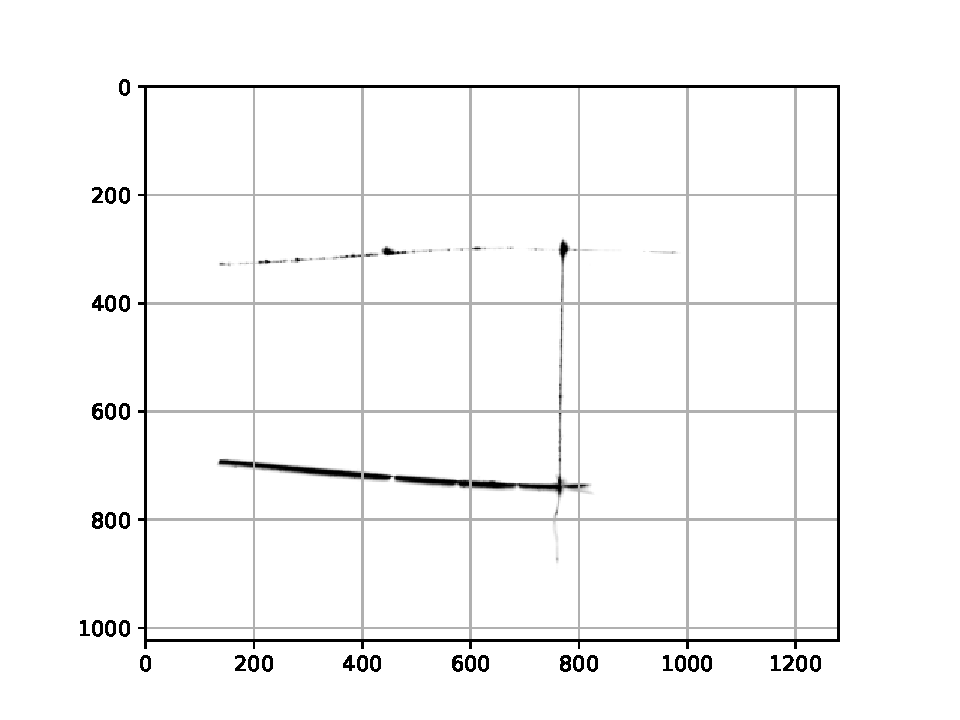
\includegraphics[width=0.6\textwidth]{	tikzs/def_075_L150_V40.pdf}	
 
	\caption{Snapshot for the body with  flexible plates..}\label{fig:snapshot}
\end{figure}

	\begin{figure}\begin{subfigure}{.49\textwidth}
		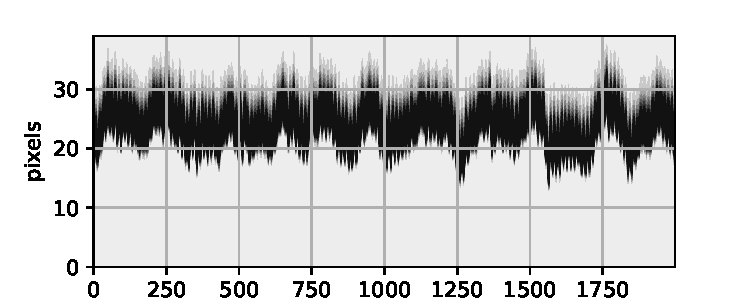
\includegraphics[width=0.9\textwidth]{tikzs/stack_t075_L150_V40_a}	
		\caption{}
		\end{subfigure}
		\begin{subfigure}{.49\textwidth}
		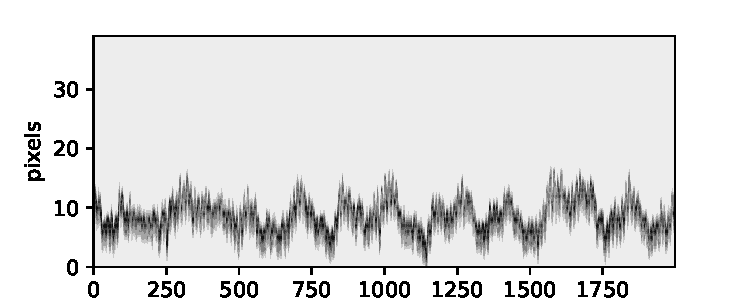
\includegraphics[width=0.9\textwidth]{tikzs/stack_t075_L150_V40_b}	
			\caption{}
		\end{subfigure}
		\caption{Stack of images for the trailing edge of the flexible plates.}\label{fig:stack}
	\end{figure}
	
\end{document}